\documentclass[12pt, a4paper]{article}

% --- Idioma, Fontes e Codificação ---
\usepackage[utf8]{inputenc}
\usepackage[T1]{fontenc}
\usepackage[brazilian]{babel}
\usepackage[autostyle=true]{csquotes}
\usepackage{lmodern}
\usepackage{csquotes}
\usepackage{booktabs}

% --- Matemática e Física ---
\usepackage{amsmath}
\usepackage{amsfonts}
\usepackage{amssymb}
\usepackage{bbm}
\usepackage{amsthm}
\usepackage{physics}
\usepackage{siunitx}
\usepackage{stmaryrd}

\DeclareMathOperator{\sgn}{sgn}
\AtBeginDocument{\RenewCommandCopy\qty\SI}
\ExplSyntaxOn
\msg_redirect_name:nnn { siunitx } { physics-pkg } { none }
\ExplSyntaxOff

% --- Elementos Gráficos e Layout ---
\usepackage{graphicx}
\usepackage{tikz}
\usepackage{float}
\usepackage{caption}
\usepackage{subcaption} 
\usepackage[top=2.5cm, bottom=2.5cm, left=3cm, right=3cm]{geometry}
\usepackage{enumitem}
\usepackage{adjustbox}
\usepackage{array}
\usepackage{algorithm}
\usepackage{algpseudocode}
\usepackage{xcolor}
\usepackage{caption}
\captionsetup{margin=1.5cm, labelfont=bf, font=small, justification=justified}

% --- Sumário, Índices e Organização ---
\usepackage{verbatim}
\usepackage{makeidx}
\usepackage{sectsty}
\usepackage{tocbibind}

% --- Bibliografia (Configuração Correta) ---
\usepackage[backend=biber,style=numeric]{biblatex}
\addbibresource{refs.bib}

% --- Teoremas e Definições ---
\newtheorem{theorem}{Teorema}[section]
\newtheorem{definition}{Definição}[section]
\newtheorem{proposition}{Proposição}[section]
\newtheorem{corollary}{Corolário}[section]

\theoremstyle{definition}
\newtheorem{example}{Exemplo}[section]

\theoremstyle{remark}
\newtheorem*{remark}{\textbf{Nota}}

% --- Customizações de Texto ---
\newcommand{\ident}{\hspace{2em}}
\renewcommand{\figurename}{Figura}
\renewcommand{\refname}{Referências}
\renewcommand{\proofname}{\normalfont\textbf{Demonstração:}}
% \renewcommand{\thedefinition}{\Roman{definition}} 
\renewcommand{\contentsname}{Sumário}

\setlength{\parindent}{0pt}
\setlength{\parskip}{0.6em}
\setlist[itemize]{leftmargin=3.0em, labelsep=0.5em}
\setlist[enumerate]{leftmargin=3.0em, labelsep=0.5em}

\floatname{algorithm}{Algoritmo}
\renewcommand{\algorithmicrequire}{\textbf{Entrada:}}
\renewcommand{\algorithmicensure}{\textbf{Saída:}}
\renewcommand{\algorithmicend}{\textbf{fim}}
\renewcommand{\algorithmicif}{\textbf{se}}
\renewcommand{\algorithmicthen}{\textbf{então}}
\renewcommand{\algorithmicelse}{\textbf{senão}}
\renewcommand{\algorithmicfor}{\textbf{para}}
\renewcommand{\algorithmicdo}{\textbf{faça}}
\renewcommand{\algorithmicwhile}{\textbf{enquanto}}
\renewcommand{\algorithmicreturn}{\textbf{retorne}}

% --- Links e Sumário Customizado ---
\usepackage{hyperref}
\hypersetup{
    colorlinks = true,
    linkcolor = black,
    urlcolor = black,
    citecolor = black
}

\makeatletter
\renewcommand\tableofcontents{
    \noindent{\Large\bfseries\contentsname}\par\vspace{0.6em} % Força o alinhamento total à esquerda
  \@mkboth{\MakeUppercase\contentsname}{\MakeUppercase\contentsname}
  \@starttoc{toc}
}

\def\algbackskip{\hskip-\ALG@thistlm}
\def\algfromtop{\vskip-\base@skip}

% Comando que desenha a linha vertical
\newcommand{\algrule}[1][0.4pt]{\vrule height .75\baselineskip depth .25\baselineskip width #1}

% Aplica a regra no início de cada linha de bloco
\newcommand{\addalgrule}{\color{gray!60}\algrule\hskip\ALG@tlm\relax}

% Intercepta os comandos do pacote para injetar as linhas
\newcommand{\StateXWithRule}{\Statex\hskip\ALG@thistlm\addalgrule}

\makeatother

\begin{document}

\begin{titlepage}
    \thispagestyle{empty}
    \centering
    
    % Cabeçalho Institucional
    \noindent
    \begin{minipage}[c]{0.18\textwidth}
        \centering
        
\includegraphics[width=\textwidth]{Imagens/logo_ufs.png} 
    \end{minipage}
    \hfill
    \begin{minipage}[c]{0.60\textwidth}
        \centering
        \fontsize{11pt}{14pt}\selectfont
        \textbf{UNIVERSIDADE FEDERAL DE SERGIPE} \\
        \textbf{CENTRO DE CIÊNCIAS E TECNOLOGIA} \\
        \textbf{DEPARTAMENTO DE MATEMÁTICA} \\
        \fontsize{10pt}{12pt}\selectfont
        \textbf{CURSO BACHARELADO EM MATEMÁTICA APLICADA E COMPUTACIONAL}
    \end{minipage}
    \hfill
    \begin{minipage}[c]{0.18\textwidth}
        \centering
        
\includegraphics[width=\textwidth]{Imagens/logo_dma.png}
    \end{minipage}

    \vfill

    % Título do Trabalho
    \begin{center}
        \fontsize{16pt}{20pt}\selectfont
        \textbf{Análise Topológica de Dados Aplicada a dados de Biologia}
    \end{center}

    \vfill

    % Autor
    \begin{center}
        \fontsize{12pt}{14pt}\selectfont
        \textbf{Autor: Anthony dos Anjos Marques}
    \end{center}

    \vfill

    % Local e Data
    \begin{center}
        \fontsize{12pt}{14pt}\selectfont
        \textbf{São Cristóvão - SE} \\
        \vspace{0.2cm}
        \textbf{Julho, 2026}
    \end{center}
\end{titlepage}


\begin{titlepage}
    \thispagestyle{empty}
    \centering
    
    % Cabeçalho Institucional Repetido
    \noindent
    \begin{minipage}[c]{0.18\textwidth}
        \centering
        
\includegraphics[width=\textwidth]{Imagens/logo_ufs.png} 
    \end{minipage}
    \hfill
    \begin{minipage}[c]{0.60\textwidth}
        \centering
        \fontsize{11pt}{14pt}\selectfont
        \textbf{UNIVERSIDADE FEDERAL DE SERGIPE} \\
        \textbf{CENTRO DE CIÊNCIAS E TECNOLOGIA} \\
        \textbf{DEPARTAMENTO DE MATEMÁTICA} \\
        \fontsize{10pt}{12pt}\selectfont
        \textbf{CURSO BACHARELADO EM MATEMÁTICA APLICADA E COMPUTACIONAL}
    \end{minipage}
    \hfill
    \begin{minipage}[c]{0.18\textwidth}
        \centering
        
\includegraphics[width=\textwidth]{Imagens/logo_dma.png}
    \end{minipage}

    \vfill

    % Título do Trabalho
    \begin{center}
        \fontsize{16pt}{20pt}\selectfont
        \textbf{Análise Topológica de Dados Aplicada a dados de Biologia}
    \end{center}

    \vfill

    % Autor
    \begin{center}
        \fontsize{12pt}{14pt}\selectfont
        \textbf{Autor: Anthony dos Anjos Marques}
    \end{center}

    \vspace{1cm}

    % Orientador(es) - Deixei o campo aberto para você preencher
    \begin{center}
        \fontsize{11pt}{13pt}\selectfont
        \textbf{Orientador:} Prof. Dr. Danilo Dias da Silva
    \end{center}

    \vspace{1cm}

    % Bloco de Notas de Monografia II do DMAT/UFS
    \noindent\hfill
    \begin{minipage}{0.55\textwidth}
        \fontsize{10pt}{13pt}\selectfont
        Trabalho de Conclusão de Curso apresentado como requisito parcial de avaliação, da disciplina Monografia II, orientado pelo Prof. Dr. Danilo Dias da Silva, no Curso de Bacharelado em Matemática Aplicada e Computacional, da Universidade Federal de Sergipe - UFS, no segundo semestre letivo de 2026.
    \end{minipage}

    \vfill

    % Local e Data
    \begin{center}
        \fontsize{12pt}{14pt}\selectfont
        \textbf{São Cristóvão - SE} \\
        \vspace{0.2cm}
        \textbf{Julho, 2026}
    \end{center}
\end{titlepage}


\newpage
\thispagestyle{empty}

\vspace*{1cm}

\begin{center}
    \fontsize{14pt}{18pt}\selectfont
    \textbf{Análise Topológica de Dados Aplicada a dados de Biologia}
\end{center}

\vspace{1.5cm}

\begin{flushleft}
    \fontsize{11pt}{14pt}\selectfont
    Trabalho de Conclusão de Curso apresentado pelo aluno Anthony dos Anjos Marques ao curso de Bacharelado em Matemática Aplicada e Computacional/DMA/UFS em 24/07/2026, como requisito de avaliação final do Trabalho de Conclusão de Curso, sob a avaliação da Banca Examinadora constituída pelos seguintes professores:
\end{flushleft}

\vspace{2cm}

% Assinaturas da Banca
\begin{center}
    \underline{\hspace{10cm}} \\
    \fontsize{10pt}{12pt}\selectfont Nome completo com titulação (orientador/a)\\
    \vspace{1.5cm}
    \underline{\hspace{10cm}} \\
    \fontsize{10pt}{12pt}\selectfont Nome completo com titulação (examinador/a convidado/a interno/a) \\
    \vspace{1.5cm}
    \underline{\hspace{10cm}} \\
    \fontsize{10pt}{12pt}\selectfont Nome completo com titulação (examinador/a convidado/a externo/a) \\
    \vspace{1.5cm}
    \underline{\hspace{10cm}} \\
    \fontsize{10pt}{12pt}\selectfont Nome completo com titulação (examinador/a suplente)
\end{center}


\newpage
\thispagestyle{empty}


\tableofcontents

\newpage

\setcounter{page}{1}

\section{Introdução}

\ident A biologia estrutural tem passado por uma revolução quantitativa nas últimas décadas, impulsionada pela necessidade de compreender não apenas a estrutura estática das macromoléculas, mas também a sua dinâmica e flexibilidade funcional. Nesse contexto, proteínas não são entidades rígidas; elas operam como nanomáquinas complexas que transitam entre diferentes estados conformacionais para exercerem suas funções biológicas, como a catálise enzimática e o transporte de ligantes. A distinção entre as teorias clássicas de interação proteína-ligante — do modelo rígido de chave-fechadura aos modelos modernos de encaixe induzido (\textit{induced fit}) e seleção conformacional (\textit{conformational selection}) — evidencia a necessidade de ferramentas matemáticas capazes de capturar a essência da dinâmica molecular.

\ident Neste contexto, a Proteína de Ligação à Maltose (MBP — \textit{Maltose-Binding Protein}), encontrada na bactéria \textit{Escherichia coli}, apresenta-se como um modelo de estudo ideal. A MBP atua no transporte de maltodextrinas e transita fundamentalmente entre duas conformações: o estado \textit{Apo} (aberto e livre de ligante) e o estado \textit{Holo} (fechado e associado ao ligante). A compreensão e a distinção exata desses estados desafiam as métricas geométricas tradicionais, como o Desvio Quadrático Médio (RMSD), que frequentemente falham em capturar correlações não-lineares sutis ou variações dinâmicas globais na estrutura da proteína.

\begin{figure}[H]
    \centering
    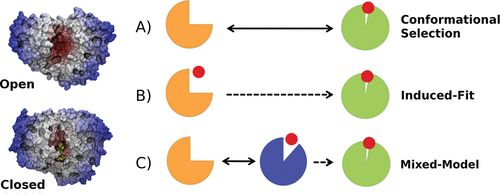
\includegraphics[width=0.8\textwidth]{Imagens/apresentacao_mbp.png}
    \caption{Representação das conformidades da MBP. 
    Fonte: Adaptado de Bucher et al.~\cite{bucher2011}.}
    
\end{figure}

\ident Para contornar as limitações da análise puramente geométrica, modelos baseados na física estatística e em simulações de grão grosso (\textit{coarse-grained}), como o Modelo de Rede Anisotrópica (ANM — \textit{Anisotropic Network Model}), tornaram-se cruciais. Ao modelar a proteína como um sistema de massas e molas, o ANM permite a construção de uma Matriz Hessiana que, após decomposição espectral e foco nos modos normais de baixa frequência, gera uma Matriz de Correlação Cruzada. Essa matriz quantifica como as flutuações de diferentes resíduos de aminoácidos estão acopladas dinamicamente, fornecendo uma ``assinatura física'' do comportamento global da macromolécula.

\ident O ponto central deste trabalho reside na transição do domínio da biofísica para o da matemática pura e aplicada, especificamente através da Análise Topológica de Dados (TDA — \textit{Topological Data Analysis}). A partir da matriz de correlação cruzada, define-se uma pseudométrica que transforma a dinâmica da proteína em um espaço métrico. Utilizando o ferramental da Homologia Persistente, filtrações de complexos simpliciais (como o Complexo de Vietoris-Rips) são construídas para acompanhar a evolução das características topológicas — componentes conexas e ciclos unidimensionais — ao longo de diferentes escalas de distância. 

\ident Diferente das abordagens clássicas, a topologia se preocupa com a forma e a conectividade intrínseca dos dados, sendo invariante a deformações contínuas. Extraímos essas assinaturas topológicas por meio de Paisagens de Persistência (\textit{Persistence Landscapes}), que mapeiam os dados topológicos, originalmente discretos e de difícil manipulação algébrica, em um espaço de funções de Banach. Esta transformação garante a estabilidade dos dados e permite a integração direta com métodos de estatística clássica e algoritmos de \textit{Machine Learning}.

\ident Por fim, com as representações topológicas traduzidas para o escopo numérico, aplica-se o Teste de Permutação para validação estatística da separabilidade das conformações, além do treinamento de um classificador supervisionado baseado em Máquinas de Vetores de Suporte (SVM — \textit{Support Vector Machines}). 

\ident Portanto, o objetivo fundamental deste trabalho é investigar, fundamentar e aplicar a Análise Topológica de Dados e a Homologia Persistente na extração de características dinâmicas de estruturas biomoleculares, utilizando a MBP como caso prático. Busca-se demonstrar que a união entre a teoria de grafos físicos (ANM) e os invariantes topológicos fornece um arcabouço rigoroso e superior para a classificação de estados proteicos.

\section{Contexto Biológico e Extração da Dinâmica Estrutural}

\ident Para que as ferramentas da Análise Topológica de Dados (TDA) possam ser aplicadas com rigor, é necessário primeiramente traduzir o comportamento físico do objeto de estudo em um espaço métrico bem definido. Nesta seção, apresentamos o sistema biológico sob análise — a Proteína de Ligação à Maltose (MBP) — e descrevemos como o Modelo de Rede Anisotrópica (ANM) é utilizado para mapear suas flutuações dinâmicas, culminando na construção de uma matriz de distâncias que servirá como substrato para as filtrações topológicas subsequentes.

\subsection{A Proteína de Ligação à Maltose (MBP)}

\ident A \textit{Maltose-Binding Protein} (MBP) é uma macromolécula essencial no sistema de captação e transporte de maltodextrinas na bactéria \textit{Escherichia coli \cite{Boos1998, spurlino1991}}. Estruturalmente, a MBP é dividida em dois domínios globulares principais interconectados por uma região de dobradiça flexível (\textit{hinge}). 

\ident A relevância da MBP para este estudo reside na sua mecânica funcional: ela atua transitando predominantemente entre dois estados conformacionais. Na ausência de um ligante, a proteína adota uma conformação \textit{Apo} (aberta). Quando há a presença e ligação do açúcar (como a maltose), ela transita para a conformação \textit{Holo} (fechada), aprisionando o substrato. Historicamente, a transição entre esses estados gerou debates entre modelos clássicos, como o Encaixe Induzido (\textit{Induced Fit}), onde o ligante força o fechamento, e a Seleção Conformacional (\textit{Conformational Selection}) \cite{bucher2011}., onde a proteína já oscila naturalmente para a forma fechada e o ligante apenas estabiliza essa forma.

\begin{figure}[H]
    \centering
    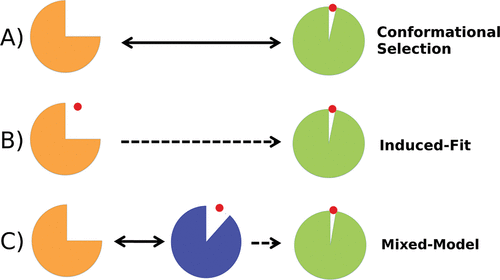
\includegraphics[width=0.8\textwidth]{Imagens/conformidade_proteina.png} 
    \caption{Representação das transições conformacionais da MBP. Da esquerda para a direita: Estado Aberto, Semi-fechado transiente e Fechado estabilizado pelo ligante (em vermelho). (A) A apoproteína é suficientemente flexível para exibir movimentos de abertura para fechamento, e o papel do ligante é estabilizar a forma fechada. (B) A proteína não ligada é incapaz de atingir a forma fechada, e a plasticidade estrutural é dependente do ligante. (C) Uma combinação das etapas A e B é necessária para atingir a conformação fechada.Fonte: Adaptado de Bucher et al.~\cite{bucher2011}.}
    \label{fig:mbp_conformations}
\end{figure}

\ident Independentemente do modelo biológico exato, o desafio matemático é claro: diferenciar essas duas classes (Aberta e Fechada) com base em suas propriedades estruturais e dinâmicas, superando métricas de alinhamento puramente rígidas e geométricas que não capturam as complexas correlações espaciais das macromoléculas em movimento.

\begin{figure}[H]
    \centering
    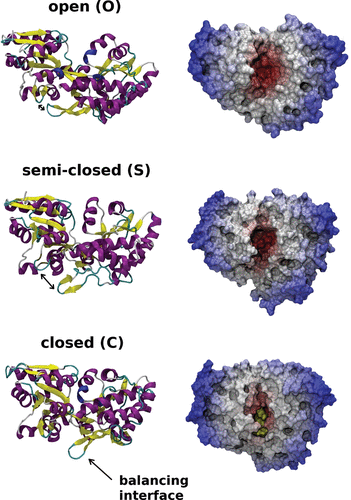
\includegraphics[width=0.5\textwidth]{Imagens/estagios_mbp_3d.png}  
    \caption{Vistas lateral e superior da MBP, mostrando o tamanho e a forma do sítio de ligação que é modulado pelo estado conformacional da proteína. A cor vermelha indica que os resíduos estão próximos ao centro de massa da proteína, onde o sítio de ligação está localizado. As estruturas de raios X são mostradas para o estado aberto não ligado (entrada PDB 1OMP) e para o estado fechado ligado (entrada PDB 3MBP). Fonte: Adaptado de Bucher et al.~\cite{bucher2011}.}  
\end{figure}

\subsection{O Modelo de Rede Anisotrópica (ANM)}

\ident Para capturar a dinâmica intrínseca da MBP sem o custo computacional proibitivo das simulações completas de Dinâmica Molecular, adota-se uma abordagem de grão grosso (\textit{coarse-grained}) baseada em física estatística: o Modelo de Rede Anisotrópica (ANM) \cite{atilgan2001}. 

\ident No ANM, a estrutura tridimensional da proteína é abstraída como um grafo espacial. Cada resíduo de aminoácido é representado unicamente por seu átomo de Carbono-alfa ($C_\alpha$), que atua como um nó neste grafo. Interações interatômicas são modeladas como um sistema de molas elásticas que conectam nós localizados dentro de um raio de corte predefinido \cite{atilgan2001}. 

\ident O comportamento deste sistema de massas e molas é governado por uma aproximação harmônica do potencial elástico da rede. A topologia física dessa rede é codificada na matriz de segundas derivadas do potencial, conhecida como Matriz Hessiana ($H$).

\begin{remark}
A dedução analítica detalhada da energia potencial, a formulação tridimensional da Matriz Hessiana $H$ e sua decomposição espectral (cálculo dos autovalores e autovetores associados aos modos normais de vibração) envolvem um forte arcabouço de física mecânica e estatística que foge ao escopo puramente topológico do texto principal. Portanto, toda a fundamentação física e algébrica do ANM encontra-se detalhada no Apêndice \ref{apx:anm}.
\end{remark}

\ident Do ponto de vista matemático para a classificação estrutural, o resultado fundamental do modelo ANM repousa na inversa pseudogeneralizada da Matriz Hessiana. A partir dos modos de baixa frequência (geralmente os 20 primeiros modos não triviais, que ditam os movimentos globais da proteína \cite{atilgan2001, kovacev2016}), constrói-se a Matriz de Correlação Cruzada ($C$). 

\ident Cada elemento $C_{ij}$ desta matriz quantifica a correlação entre as flutuações vetoriais do resíduo $i$ e do resíduo $j$. Valores de $C_{ij}$ próximos a $1$ indicam movimentos altamente correlacionados (na mesma direção), próximos a $-1$ indicam movimentos anticorrelações (direções opostas), e valores próximos a $0$ indicam ausência de correlação dinâmica \cite{kovacev2016}.

\subsection{Construção do Espaço Métrico}

\ident A Análise Topológica de Dados opera sobre espaços de pontos equipados com uma noção formal de distância. A Matriz de Correlação Cruzada $C$ é rica em informação dinâmica, mas não satisfaz os axiomas de uma métrica geométrica. Para viabilizar a análise topológica, aplica-se uma transformação que mapeia correlações em distâncias.

\ident Definimos a distância dinâmica $D_{ij}$ entre os resíduos $i$ e $j$ através da relação:
\begin{equation}
    D_{ij} = 1 - |C_{ij}|
\end{equation}
\ident Com esta formulação, resíduos que possuem comportamentos dinâmicos altamente acoplados ($|C_{ij}| \to 1$) apresentarão uma distância dinâmica próxima a zero ($D_{ij} \to 0$), indicando que, topologicamente e funcionalmente, eles estão ``próximos''. Inversamente, resíduos com dinâmicas independentes estarão distantes neste novo espaço métrico.

\ident A matriz de distâncias dinâmicas $D$ constitui o ponto de partida matemático deste trabalho. Ela nos permite abandonar as coordenadas euclidianas estáticas $(x, y, z)$ da biologia clássica e passar a tratar a proteína como um espaço métrico discreto, sobre o qual definiremos complexos simpliciais e calcularemos grupos de homologia persistente nos próximos capítulos. É crucial notar que $\mathbf{D}$ não é estritamente uma métrica, mas sim uma pseudométrica. Isto ocorre porque a identidade dos indiscerníveis não se verifica rigorosamente: dois resíduos distintos ($i \neq j$) podem oscilar de forma perfeitamente correlacionada ($|C_{ij}| = 1$), resultando numa distância $D_{ij} = 0$. Por outro lado, é possível demonstrar a desigualdade triangular é satisfeita, isto é, $D_{ij}\leq D_{ik} + D_{kj}$. A Topologia Algébrica, contudo, é perfeitamente bem definida sobre espaços pseudométricos, permitindo a construção de complexos simpliciais sem perda de generalidade teórica.


\section{Fundamentos de Topologia Algébrica e Homologia Persistente} \label{sec:homologia_persistente}

\ident O estabelecimento de uma matriz de distâncias (ou pseudodistâncias) a partir de um sistema dinâmico fornece um espaço métrico discreto. Para extrair a arquitetura de comunicação global da biomolécula a partir desta pseudométrica, traduzimos este espaço num objeto combinatório contínuo. Nesta seção, fundamentamos o arcabouço matemático necessário para essa transição, introduzindo conceitos da Topologia Algébrica e da Homologia Persistente, usando como base o conteúdo de Tinarrage \cite{tinarrage2021}.

\subsection{Complexos Simpliciais} 

\ident Espaços topológicos, como subconjuntos de $\mathbb{R}^n$, podem ser difíceis de manipular computacionalmente. Para descrevê-los de forma adequada, podemos tentar decompô-los em partes mais simples, uma generalização de grafos para dimensões superiores que permite a representação de espaços topológicos de forma combinatorial. As partes que consideraremos são os simplexos padrão. Lembramos que o simplexo padrão de dimensão $n$ é o seguinte subconjunto de $\mathbb{R}^{n+1}$. 
\begin{align*}
    \Delta_n = \left\{x = \left(x_1, \dots\ x_{n+1}\right) \in \mathbb{R}^{n+1} \mid x \geq 0 \ \text{e} \ \sum_{i=1}^{n+1}x_i=1\right\}.
\end{align*}

\begin{definition}\label{fecho_convexo}
    Para qualquer conjunto de pontos $a_1, \dots, a_k \in \mathbb{R}^n$, definimos seu fecho convexo como:
    \begin{align*}
        \textup{conv}({a_1, ..., a_k}) = \left\{\sum_{1\leq i \leq k} t_i a_i\mid \sum_{j = 1}^{k} t_j = 1, t_j \geq 0 \right\}.
    \end{align*}
    Portanto, podemos dizer que $\Delta_n$ é o fecho convexo dos vetores $e_1, \dots, e_{n+1} \in \mathbb{R}^{n+1}$, onde
    \begin{align*}
        e_i = (0, \dots, 1, 0, \dots, 0) \quad \textup{(i-ésima coordenada igual a 1, as demais iguais 0)}.
    \end{align*}
\end{definition}

\begin{definition}[Complexo Simplicial]
Seja $V$ um conjunto (chamado de conjunto de vértices). Um complexo simplicial sobre $V$ é um conjunto $K$ de subconjuntos de $V$ (chamados de simplexos) tal que, para todo $\sigma \in K$ e todo $\tau \subset \sigma$ não-vazio, temos $\tau \in K$.
\end{definition}

\ident Atualmente, um complexo simplicial não possui topologia. É um objeto puramente combinatório. No entanto, para representá-lo, podemos desenhá-lo da seguinte forma: coloque os pontos $V$ no plano ou no espaço e, para cada simplexo de $K$, preencha o casco convexo de seus vértices. Podemos visualizar os simplexos das seguintes formas geométricas:

\begin{figure}[H]
    \centering
    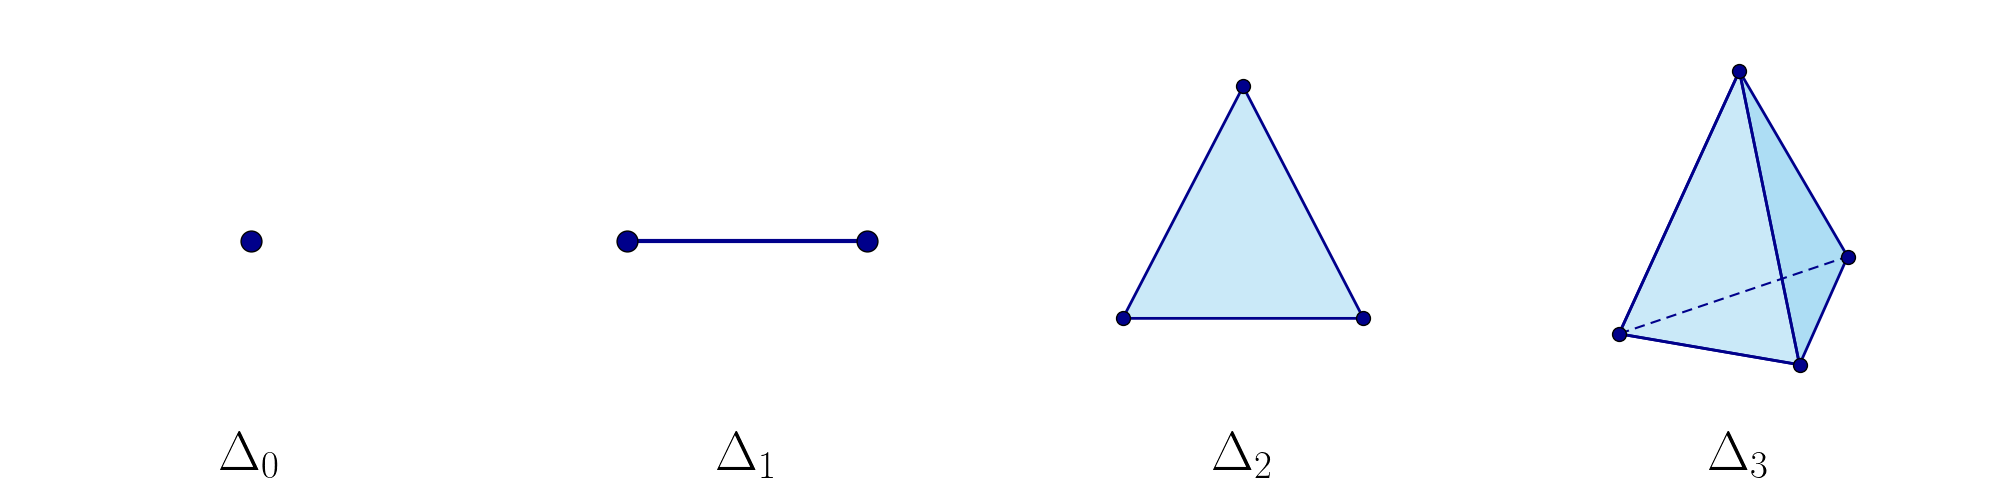
\includegraphics[width=1\textwidth]{Imagens/definicao_simplices.png}
    \vspace{0.1em}
    \caption{Representação dos simplexos: 0-Simplexo (Ponto ou vértice), 1-Simplexo (Segmento ou aresta), 2-Simplexo (Triângulo com face preenchida) e 3-Simplexo (Tetraedro preenchido).}
\end{figure}

Note que o simplexo $\Delta_n$ é descrito por $n + 1$ vértices. Vamos manter essa imagem geométrica em mente no que se segue.

\ident Por convenção, ao falar de simplexos, usamos colchetes em vez de chaves. Por exemplo, o simplexo ${0, 1}$ será denotado por $[0, 1]$. 


\ident Se $\sigma \in K$ é um simplexo, seus subconjuntos não vazios $\tau \subset \sigma$ são chamados de faces de $\sigma$, e $\sigma$ é chamado de coface de $\tau$. Por exemplo, $[0, 1]$ é uma face de $[0, 1, 2]$, e $[0, 1, 2]$ é uma coface de $[0, 1]$.

\begin{example}\label{ex_3_1}
    Seja $V = \{0, 1, 2\}$ e
    \begin{align*}
        K = \left\{ [0], [1], [2], [0, 1], [1, 2], [2, 0]\right\}.
    \end{align*}
    É um complexo simplicial de dimensão 1, onde todos os vértices se ligam. Pode ser representado dessa forma:

    \begin{figure}[H]
        \centering
        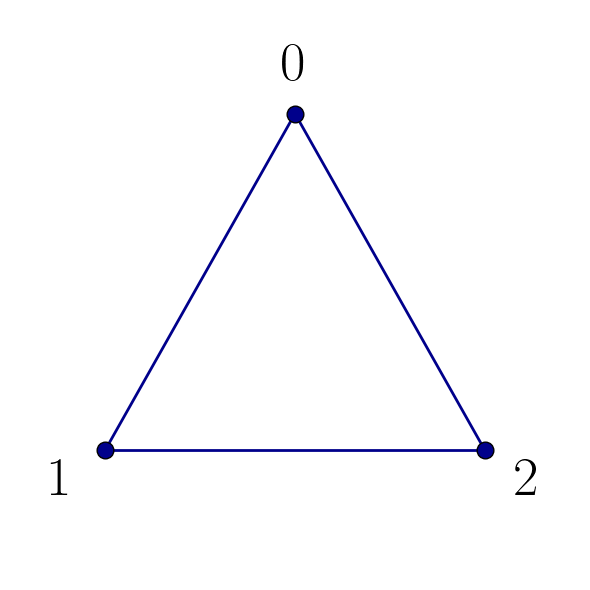
\includegraphics[width=0.3\textwidth]{Imagens/exemplo_3_1.png}
        \caption{Simplexo de dimensão 1}
    \end{figure}
\end{example}

\begin{example}
    Seja $V = \{0, 1, 2\}$ e 
    \begin{align*}
    K = \left\{[0], [1], [2], [0, 1], [1, 2], [0, 1, 2]\right\}.    
    \end{align*}
    Este não é um complexo simplicial. De fato, o simplexo $[0, 1, 2]$ admite uma face $[2, 0]$ que não está incluída em $V$.
\end{example}

\ident Se $\sigma$ é um simplexo, sua dimensão é definida como $|\sigma|-1$ (cardinalidade de $\sigma$ menos 1). Se $K$ é um complexo simplicial, sua dimensão é definida como a dimensão máxima de seus simplexo.

\begin{remark}
    Ao desenhar um complexo simplicial, os simplexos não devem se cruzar. No entanto, nem sempre é possível desenhar um complexo simplicial no plano (ou espaço) dessa maneira. Como exemplo, o grafo bipartido $K_{3,3}$ é um complexo simplicial de dimensão 1 (um grafo) que não pode ser desenhado no plano sem se cruzar.
\end{remark}

\begin{definition}
    Seja $K$ um complexo simplicial com conjunto de vértices $V=\left\{ 1, \dots, n \right\}$. Em $\mathbb{R}^{n+1}$, considere, para cada $i \in \left\{ 0, \cdots, n \right\}$, o vetor $e_i = (0, \dots, 1, 0, \\ \dots, 0)$ (com a $i$-ésima coordenada igual a $1$ e as demais iguais a $0$). Seja $|K|$ o subconjunto de $\mathbb{R}^{n+1}$ definido por:
    \begin{align*}
        |K| = \bigcup_{\sigma \in K} \textup{conv}(\{e_j, j \in \sigma\})
    \end{align*}
    onde $\textup{conv}$ representa o fecho convexo (Definição \ref{fecho_convexo}).
    Munido da topologia de subespaço, $(|K|, \tau_{|K|})$ é um espaço topológico, que denominamos realização topológica de $K$.
    
\end{definition}

\begin{definition}
    Seja $(X, \mathcal{T})$ um espaço topológico. Uma triangulação de $X$ é um complexo simplicial $K$ tal que sua realização topológica $(|K|, \mathcal{T}_{|K|})$ é homeomorfa a $(X, \mathcal{T})$.
\end{definition}

\begin{example}
    Seguindo exemplo \ref{ex_3_1}, o complexo simplicial $K$ é a triangulação de um círculo.
\end{example}

\ident Dado um espaço topológico, nem sempre é possível obter sua triangulação No entanto, quando isso é possível, existem muitas triangulações diferentes. Por exemplo, todos os seguintes complexos simpliciais são triangulações equivalentes de um círculo.

\begin{figure}[H]
    \centering
    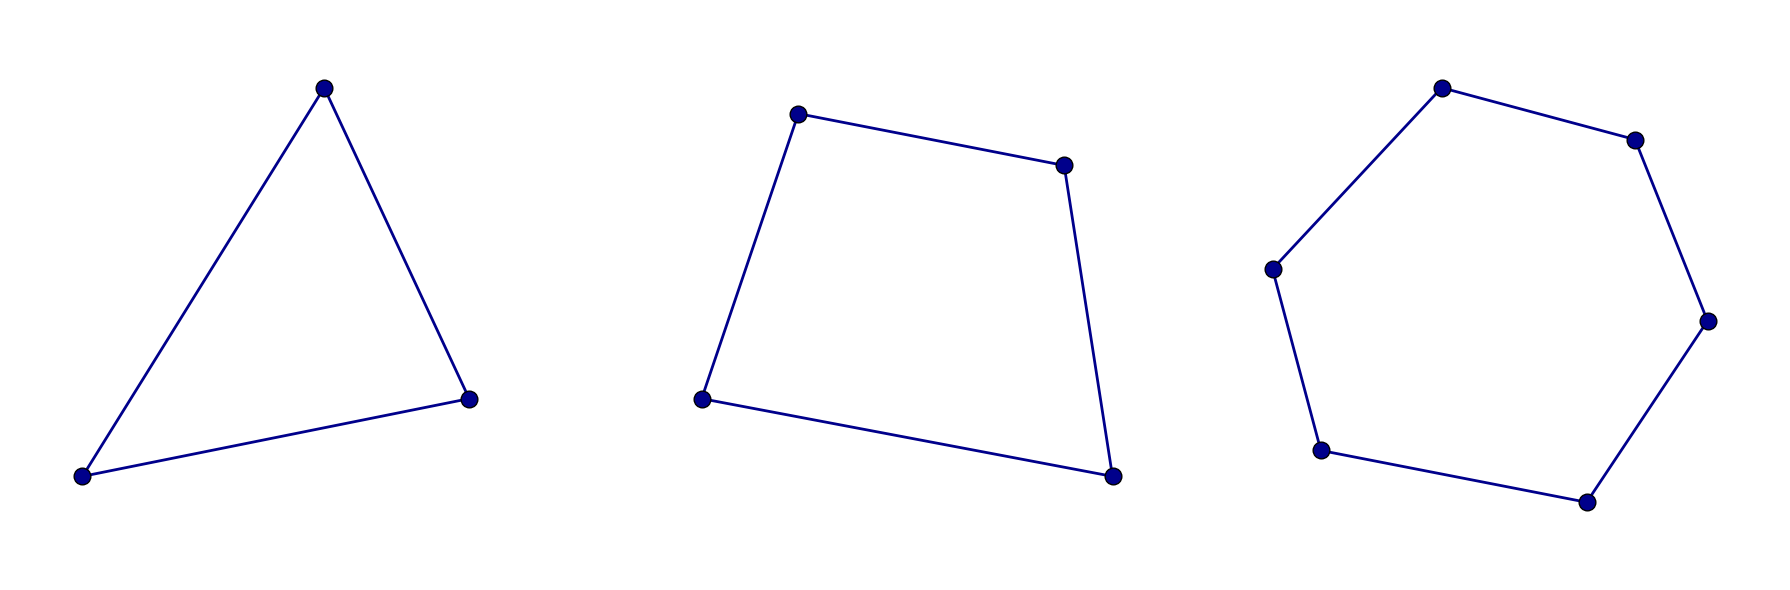
\includegraphics[width=0.8\textwidth]{Imagens/triangulacao_circulo.png}
    \caption{Triangulações de um círculo}
\end{figure}
Também podemos visualizar a triangulação de um Toro abaixo:
\begin{figure}[H]
    \centering
    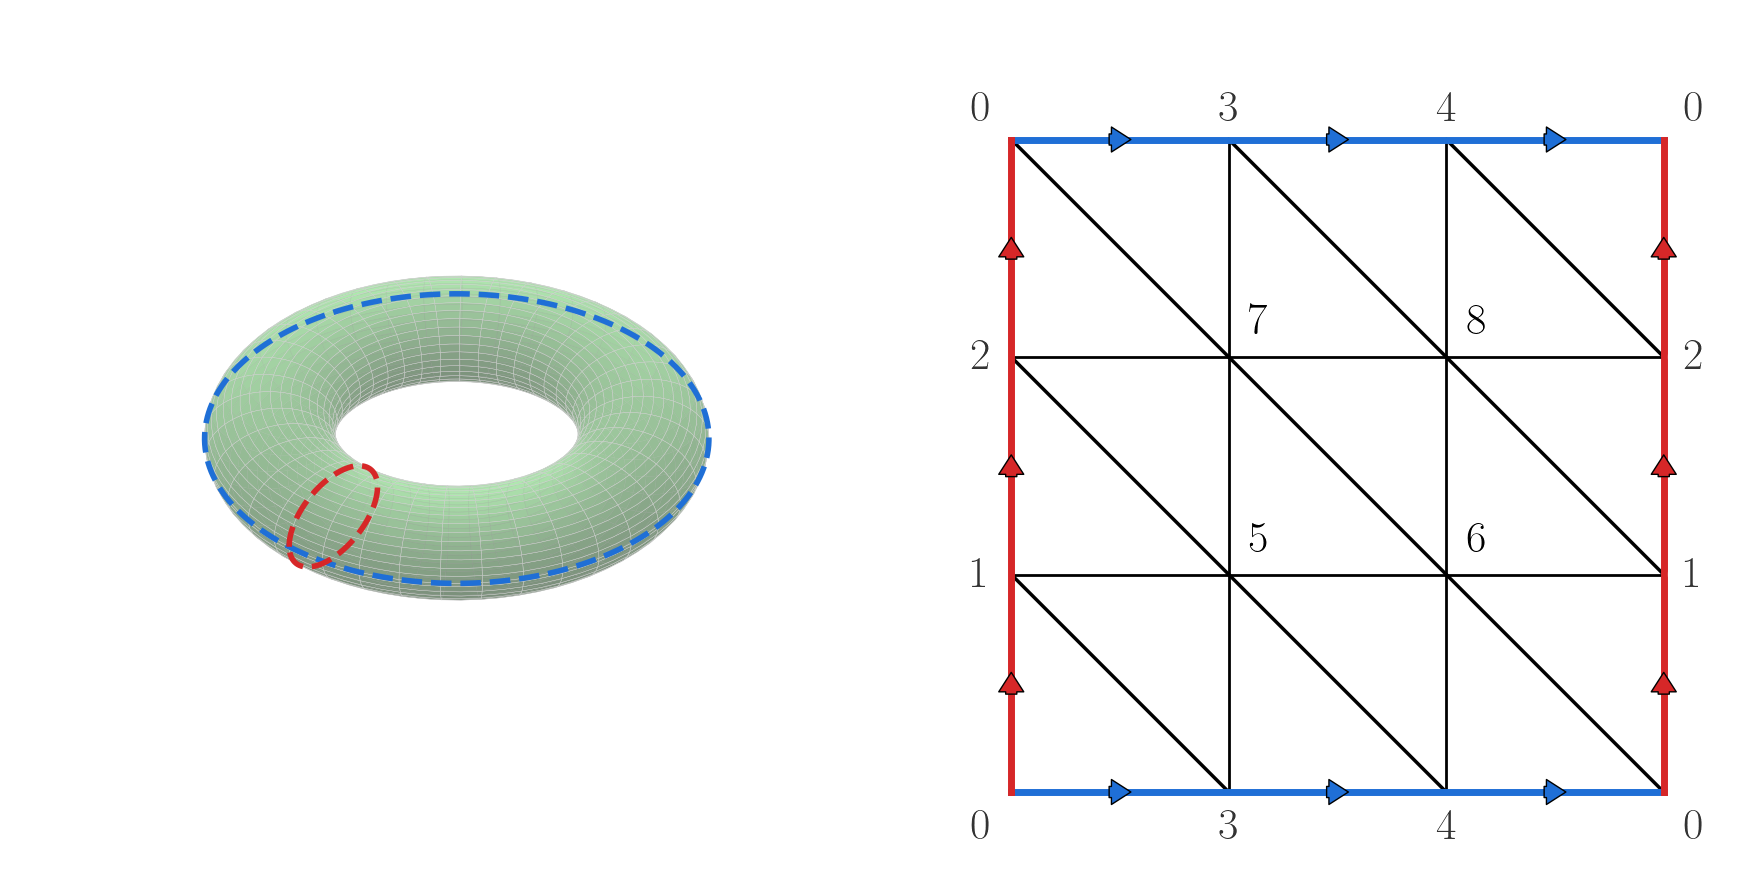
\includegraphics[width=0.8\textwidth]{Imagens/triangulacao_toru.png}
    \caption{A esquerda um Toro com dois cortes de identificação: o corte transversal (azul) que está em volta do eixo central e um corte sagital (vermelho) que está em torno do tubo. Cortar o toro nesses dois círculos, nessa ordem, reverte exatamente o processo de colagem: o corte azul primeiro abre o toro em um cilindro, e o corte vermelho em seguida abre o cilindro em um retângulo. A direita vemos a planificação do toro, as setas indicam a orientação das identificações: arestas azuis (topo/base) e vermelho (laterais) são percorridas no mesmo sentido em lados opostos, o que caracteriza a identificação de um toro.}
\end{figure}
\subsection{Grupos de Homologia}

\ident Seja $K$ um complexo simplicial abstrato. Para $n \geq 0$, definimos os conjuntos:
\begin{align*}
    K_n &= \{\sigma \in K \mid \dim(\sigma) \leq n\}\\
    K_{(n)} &= \{\sigma \in K \mid \dim(\sigma) = n\}. 
\end{align*}
O primeiro conjunto é um complexo simplicial, chamado de $n$-esqueleto de $K$. O segundo não é um complexo simplicial em geral.

\begin{figure}[H]
    \centering
    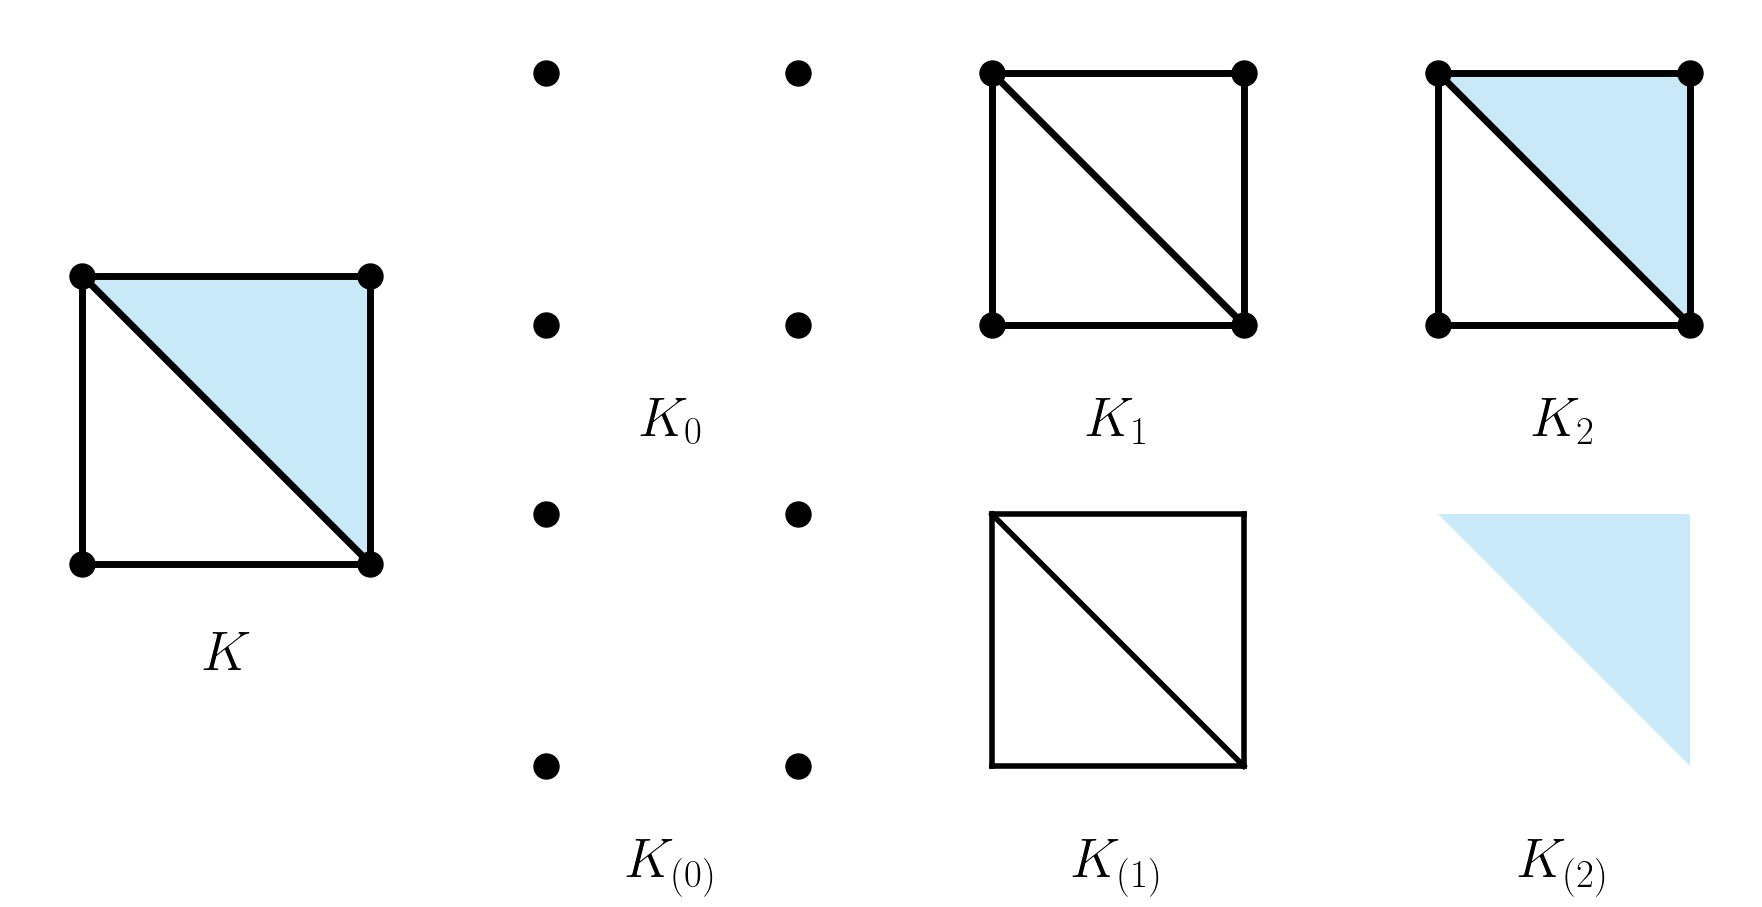
\includegraphics[width=0.8\textwidth]{Imagens/esqueleto_simplexo.png}
    \caption{Exemplo do complexo simplicial $K_n$ e o conjunto $K_{(n)}$}
\end{figure}

\ident Para extrair invariantes topológicos de um complexo simplicial, é necessário dotá-lo de uma estrutura algébrica que nos permita operar formalmente sobre os seus simplexos.

\begin{definition}[n-Cadeias]
Seja $K$ um complexo simplicial e $n \geq 0$. O conjunto de $n$-cadeias de $K$, denotado $C_n(K)$, é o conjunto cujos elementos são as somas formais:
\[
\sum_{\sigma \in K_{(n)}} \epsilon_\sigma \cdot \sigma, \quad \text{onde } \forall \sigma \in K_{(n)},\; \epsilon_\sigma \in \mathbb{Z}/2\mathbb{Z}.
\]
Este conjunto possui estrutura de espaço vetorial sobre o corpo $\mathbb{Z}/2\mathbb{Z}$, com a adição a ocorrer componente a componente.
\end{definition}

\begin{example}
    Considere o complexo simplicial 
    \begin{align*}
        K = \left\{[0], [1], [2], [0, 1], [0, 2]\right\}.
    \end{align*}
    
    As 0-cadeias $C_0(K)$ consistem em 8 elementos:
    \begin{align*}
        C_0(K) = \left\{0, [0], [1], [2], [0] + [1], [0] + [2], [1] + [2], [0] + [1] + [2]\right\}
    \end{align*}
    \begin{figure}[H]
        \centering
        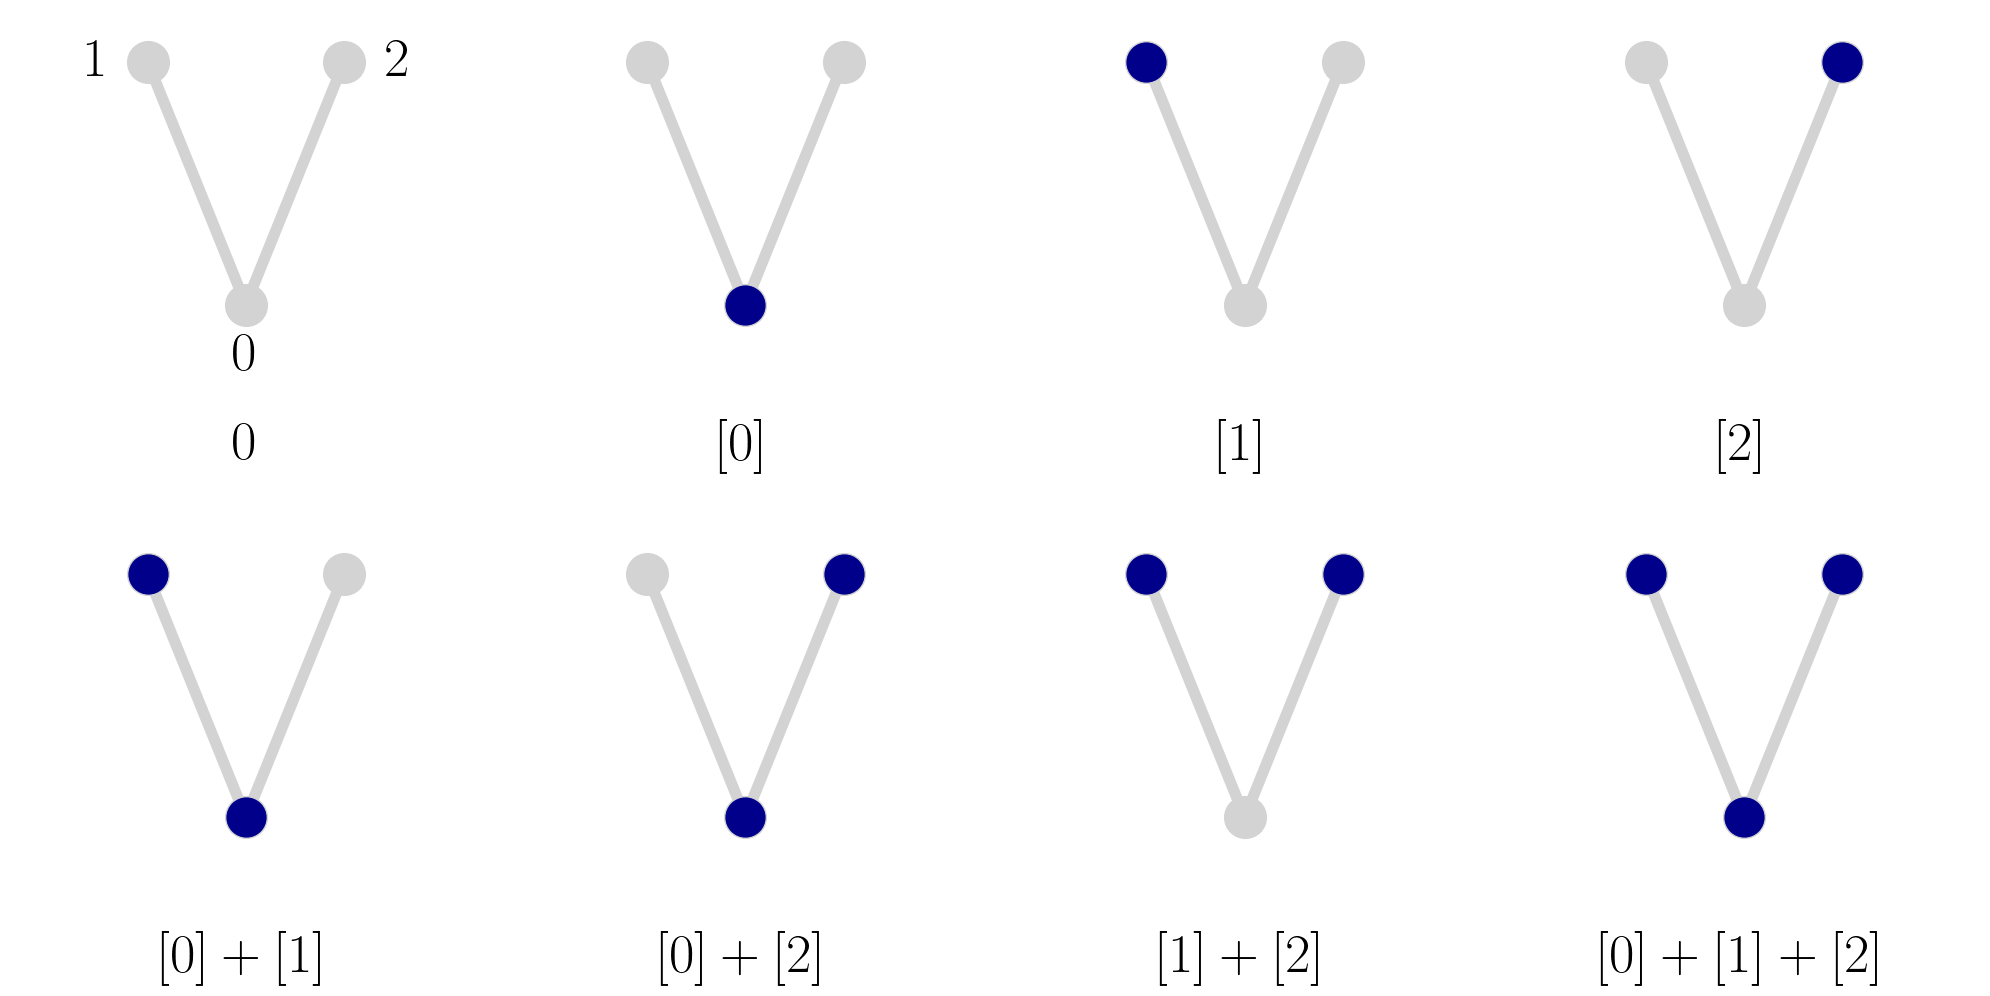
\includegraphics[width=0.8\textwidth]{Imagens/fases_n_cadeias.png}
    \end{figure}

    Por exemplo, em $C_0(K)$, temos
    \begin{align*}
        ([0] + [1]) + ([0] + [2]) = [0] + [0] + [1] + [2] = [1] + [2].
    \end{align*}
    
    Além disso, as 1-cadeias $C_1(K)$ consistem em 4 elementos:
    \begin{align*}
        C_1(K) = \left\{0, [0, 1], [0, 2], [0, 1] + [0, 2]\right\}.
    \end{align*}
    \begin{figure}[H]
        \centering
        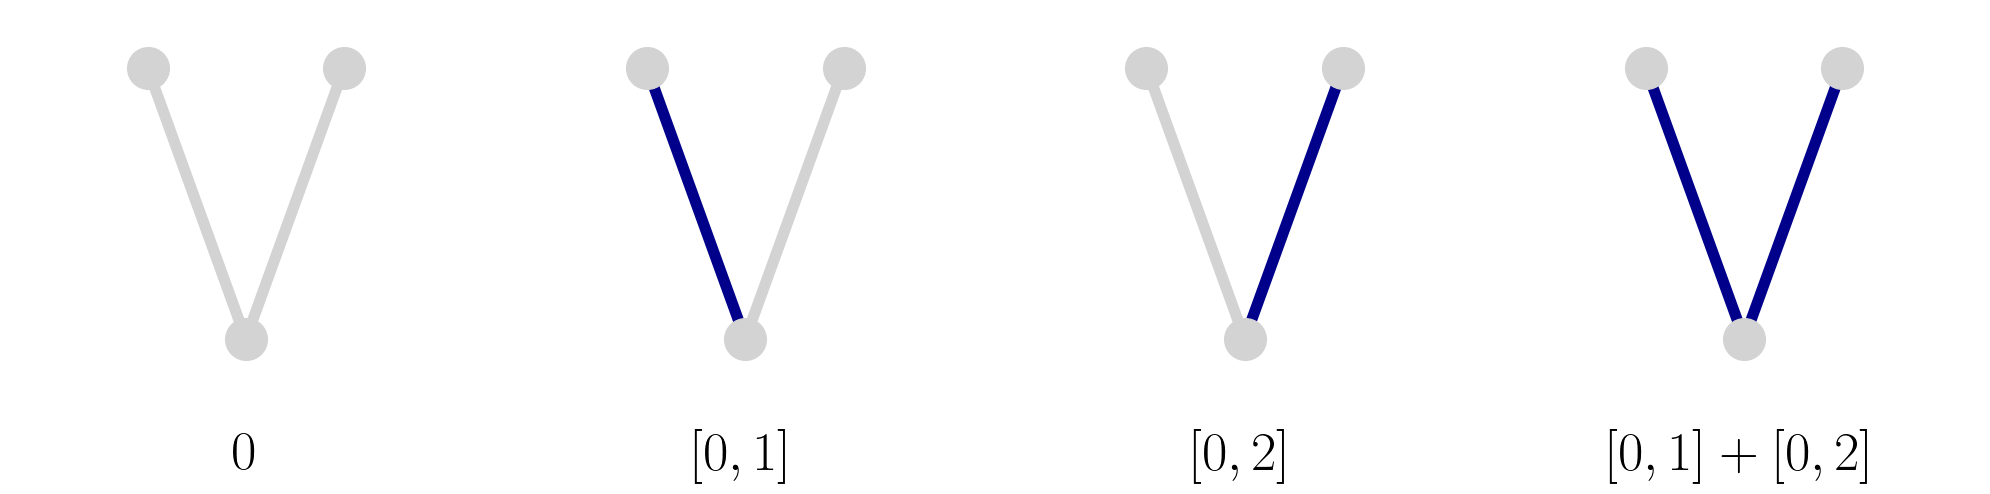
\includegraphics[width=0.8\textwidth]{Imagens/fases_n_cadeias1.png}
    \end{figure}
\end{example}

\begin{definition}[Operador de Fronteira]
Seja $n \geq 1$ e $\sigma = [x_0, \ldots, x_n] \in K_{(n)}$ um símplexo de dimensão $n$. A fronteira de $\sigma$ é o elemento de $C_{n-1}(K)$ definido por:
\[
\partial_n \sigma = \sum_{\substack{\tau \subset \sigma \\ |\tau| = |\sigma| - 1}} \tau.
\]
O operador $\partial_n$ estende-se por linearidade a uma aplicação linear $\partial_n: C_n(K) \to C_{n-1}(K)$. Para $n = 0$, define-se $\partial_0$ como a aplicação nula.
\end{definition}

\begin{example}\label{exemplo_fronteira}
    Considere o complexo simplicial
    \begin{align*}
        K = \{[0], [1], [2], [3], [0, 1], [0, 2], [1, 2], [1, 3], [2, 3], [0, 1, 2]\}.
    \end{align*}
    O simplexo $[0, 1]$ tem as faces $[0]$ e $[1]$. Logo,
    \begin{align*}
        \partial_1 [0, 1] = [0] + [1].
    \end{align*}
    \begin{figure}[H]
        \centering
        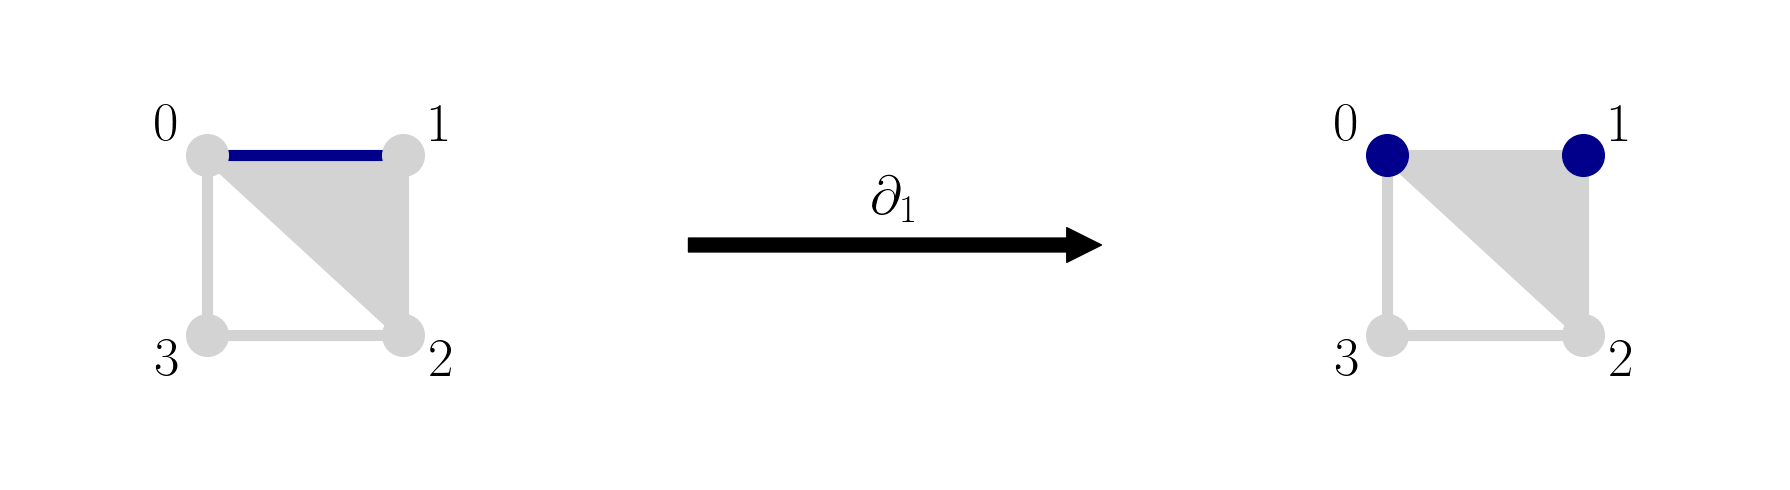
\includegraphics[width=0.8\textwidth]{Imagens/fronteiras_ex1.png}
    \end{figure}
    De modo semelhante, a fronteira da 1-cadeia $ [0, 1] + [1, 2] + [2, 0]$ é
    \begin{align*}
        \partial_1\left([0, 1] + [1, 2] + [2, 0]\right) &= \partial_1[0, 1] + \partial_1[0, 2] + \partial_1[2, 0]\\
        &= [0] + [1] + [0] + [2] + [2] + [0]\\
        &= 0
    \end{align*}
    uma vez que $[0] + [0] = [1] + [1] = [2] + [2] = 0$ em $C_0(K)$.
    \begin{figure}[H]
        \centering
        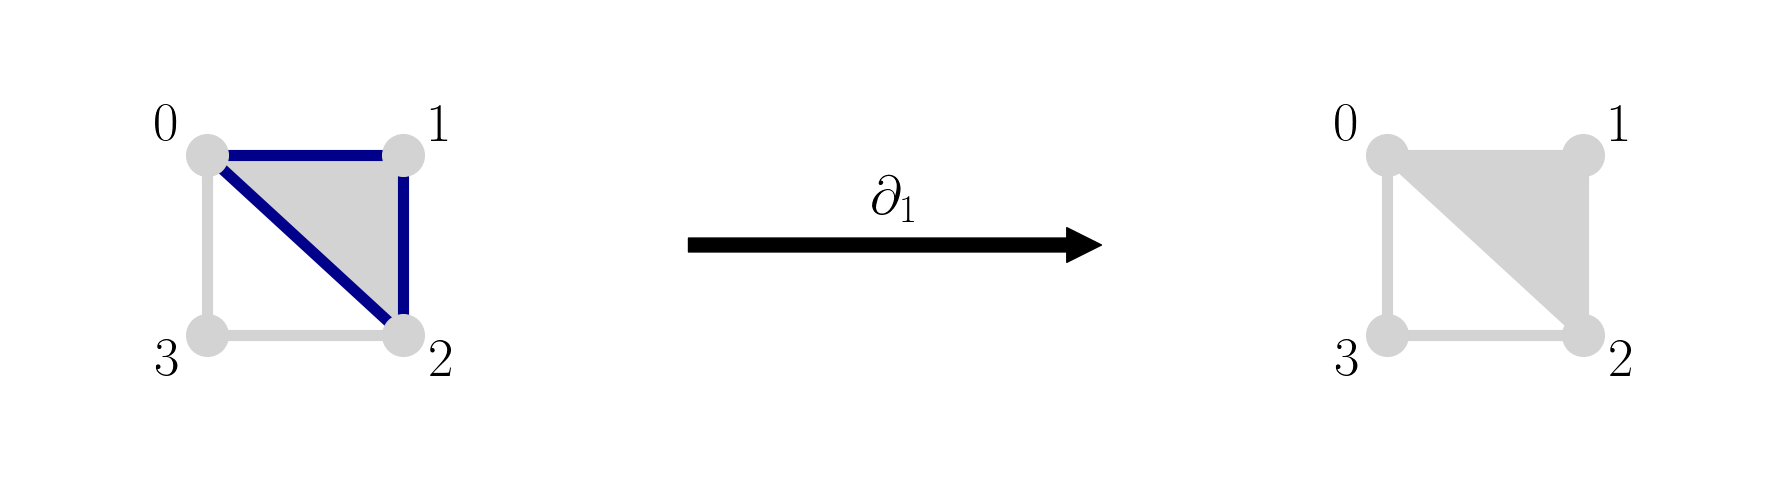
\includegraphics[width=0.8\textwidth]{Imagens/fronteiras_ex2.png}
    \end{figure}
    O simplexo $[0, 1, 2]$ possui as faces $[0, 1], [1, 2]$ e $[2, 0]$. Logo, 
    \begin{align*}
        \partial_2[0, 1, 2] = [0, 1] + [1, 2] + [2, 0].
    \end{align*}
    \begin{figure}[H]
        \centering
        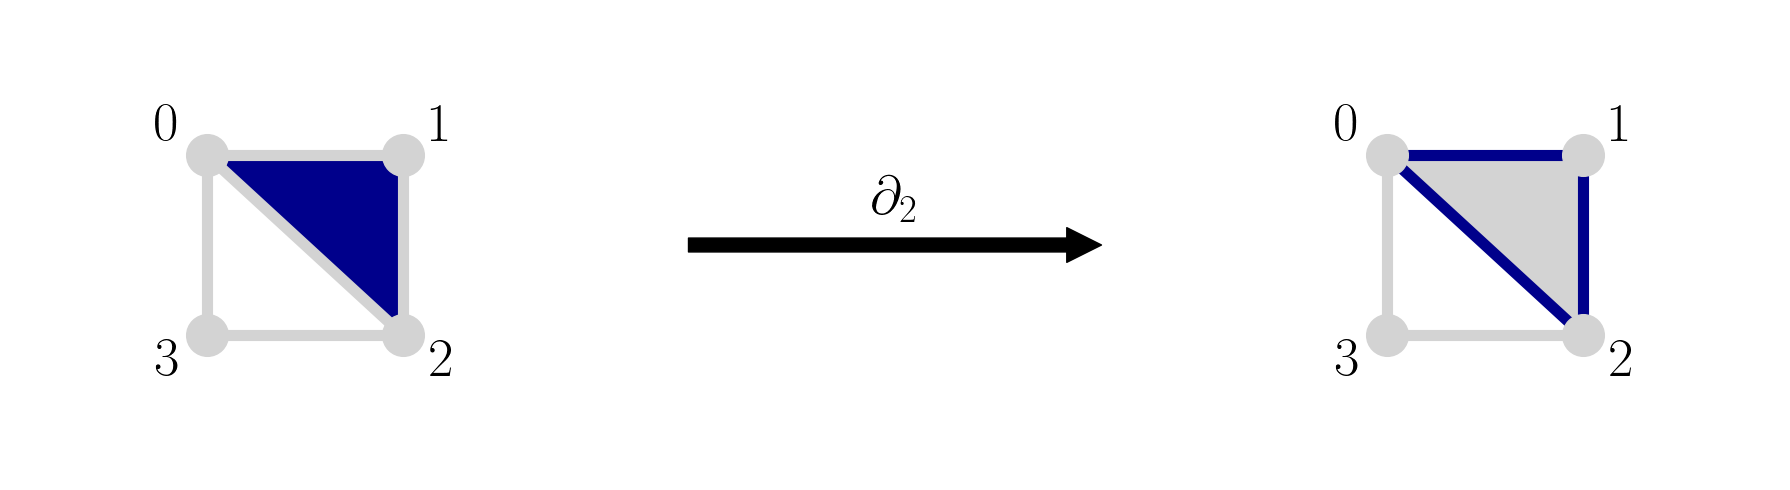
\includegraphics[width=0.8\textwidth]{Imagens/fronteiras_ex3.png}
    \end{figure}
\end{example}

\ident A aplicação linear de fronteira $\partial_n$ satisfaz a propriedade fundamental da topologia algébrica: $\partial_{n-1} \circ \partial_n = 0$. Esta identidade categórica permite-nos definir subespaços cruciais para o estudo das formas.

\begin{definition}[Ciclos e Fronteiras]
Sejam $K$ um complexo simplicial e $n \geq 0$. Definimos:
\vspace{-0.6em}
\begin{itemize}
    \item Os $n$-ciclos: $Z_n(K) = \ker(\partial_n) \subset C_n(K)$,
    \item As $n$-fronteiras: $B_n(K) = \mathrm{Im}(\partial_{n+1}) \subset C_n(K)$.
\end{itemize}
\end{definition}
\begin{example}
    Considere o complexo simplicial do Exemplo \ref{exemplo_fronteira}. O conjunto de ciclos $Z_1(K)$ consiste nas cadeias
    \begin{align*}
        0, \quad [0, 1] + [1, 2] + [0, 2], \quad [0, 2] + [2, 3] + [0, 3] \quad \text{e} \quad [0, 1] + [1, 2] + [2, 3] + [0, 3].
    \end{align*}
    As únicas fronteiras $B_1(K)$ são dadas por
    \begin{align*}
        \partial_2(0) = 0 \quad \text{and}\quad \partial_2([0, 1, 2]) = [0, 1] + [0, 2] + [1, 2].
    \end{align*}
    Vemos que as cadeias $[0, 2] + [2, 3] + [0, 3]$ e $[0, 1] + [1, 2] + [2, 3] + [0, 3]$ são homólogas.
    De fato,
    \begin{align*}
        [0, 2] + [2, 3] + [0, 3] = [0, 1] + [1, 2] + [2, 3] + [0, 3] + [0, 1] + [0, 2] + [1, 2].
    \end{align*}
    \begin{figure}[H]
        \centering
        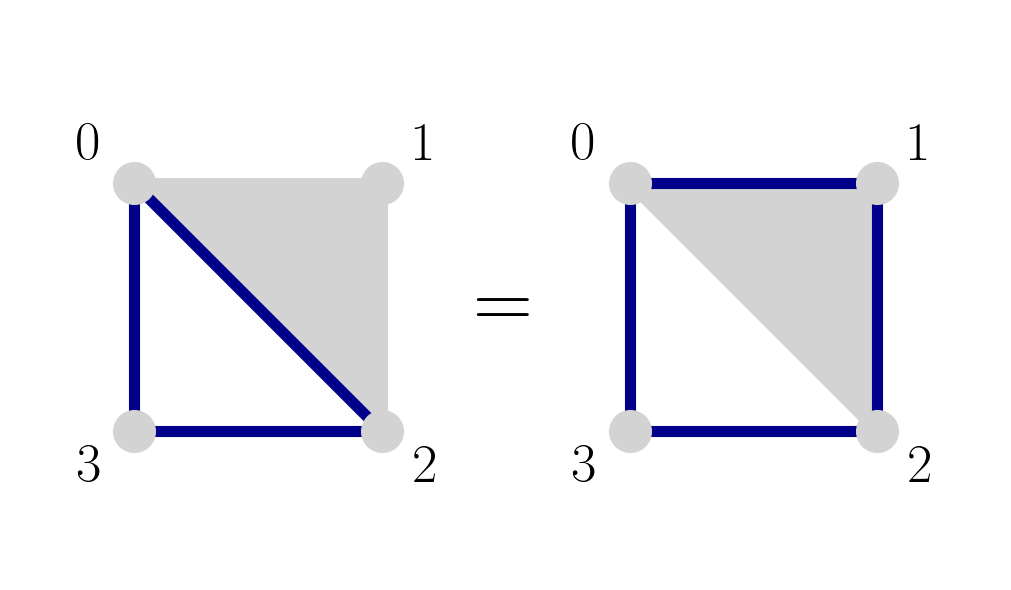
\includegraphics[width=0.6\textwidth]{Imagens/igualdade_cilcos_fronteiras.png}
    \end{figure}
\end{example}

\begin{corollary}
    Temos $B_n(K) \subset Z_n(K)$. Em outras palavras, toda fronteira é um ciclo.
\end{corollary}
\vspace{-0.6em}
Demonstração em Tinarrage \cite{tinarrage2021}.

\begin{definition}[Grupo de Homologia e Números de Betti]
    Seja $K$ um complexo simplicial. O $n$-ésimo grupo de homologia de $K$ é o quociente:
    \begin{align*}
        H_n(K) = Z_n(K) / B_n(K).
    \end{align*}
    A dimensão deste espaço vetorial é o $n$-ésimo número de Betti, dado por $\beta_n(K) = \dim H_n(K) = \dim Z_n(K) - \dim B_n(K)$. Geometricamente, $\beta_0$ conta o número de componentes conexas, $\beta_1$ o número de \enquote{buracos} ou ciclos unidimensionais, e $\beta_2$ o número de cavidades fechadas.
\end{definition}
\begin{figure}[H]
    \centering
    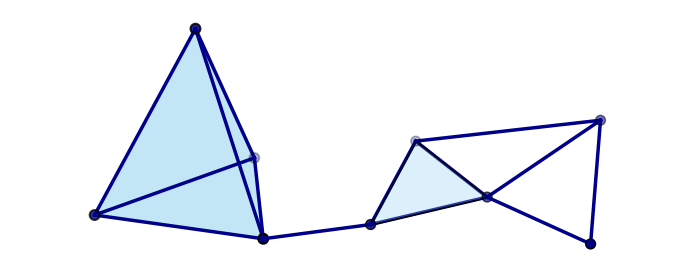
\includegraphics[width=0.8\textwidth]{Imagens/exemplo_n_betti.png}
    \caption{Note que neste simplexo temos $\beta_0 = 1 $ (1 componente conexa), $\beta_1 = 2$ (2 buracos de dimensão 1 ou 2 triângulos não preenchidos) e $\beta_2 = 1$ (1 buracos de dimensão 2 ou 1 tetraedro não preenchido/oco).}
\end{figure}

\subsection{Inferência Topológica}

\ident Na prática computacional, os dados raramente se apresentam nativamente como um complexo simplicial. Em vez disso, dispomos de nuvens de pontos em um espaço métrico. Para conectar a geometria dos dados com a topologia, utilizamos coberturas abertas e o Teorema do Nervo. Pensemos em subconjunto euclidiano finito $X\subset \mathbb{R}^n$ como sendo uma amostra de um objeto contínuo, $\mathcal{M} \subset \mathbb{R}^n$. Compreender a topologia de $\mathcal{M}$ nos daria um conhecimento interessante sobre o conjunto de dados $X$.

\begin{figure}[H]
        \centering
        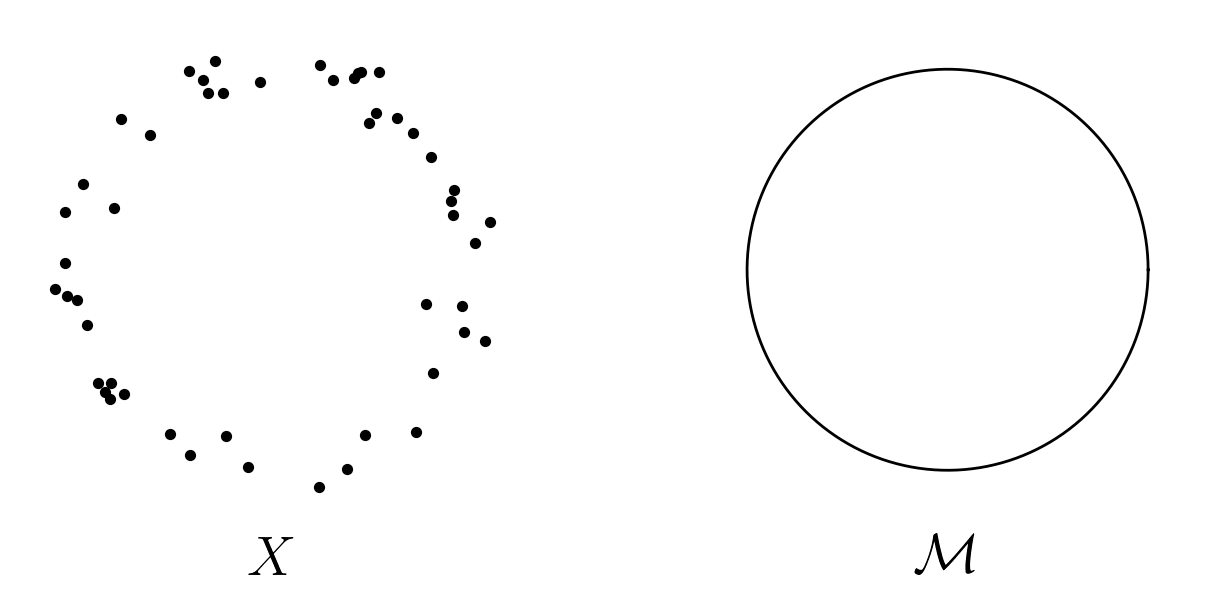
\includegraphics[width=0.6\textwidth]{Imagens/nuvem_pontos_e_circulo.png}
\end{figure}
\ident Seja $\mathcal{M}\subset \mathbb{R}^n$ um subconjunto limitado, suponha que tenhamos uma amostra finita $X\subset\mathcal{M}$. Com a Homologia Persistente, pretendemos compreender a topologia de $\mathcal{M}$ através da sua homologia. Tentaremos estimar os grupos de homologia de $\mathcal{M}$ para $X$. Infelizmente, a homologia de $X$ está muito longe da homologia de $\mathcal{M}$. No entanto, se é amostrado perto o suficiente de $\mathcal{M}$, existe uma construção que permite recuperar o tipo de homotopia de $\mathcal{M}$ para $X$, daí também seus grupos de homologia. Esta construção consiste no espessamento de $X$.


\begin{definition}[t-espessamento]
    Seja $X \subset \mathbb{R}^n$ e $t \geq 0$. O $t$-espessamento de $X$, denotado $X^t$, é o conjunto de pontos do espaço ambiente com o máximo de distância $t$ de $X$:
    \[
    X^t = \{y \in \mathbb{R}^n \mid \exists x \in X,\, \|x - y\| \leq t\} = \bigcup_{x \in X} \overline{\mathcal{B}}(x, t).
    \]
    Lê-se que $X^t$ é uma união de bolas fechadas centradas em cada ponto de $X$.

\end{definition}
\begin{figure}[H]
        \centering
        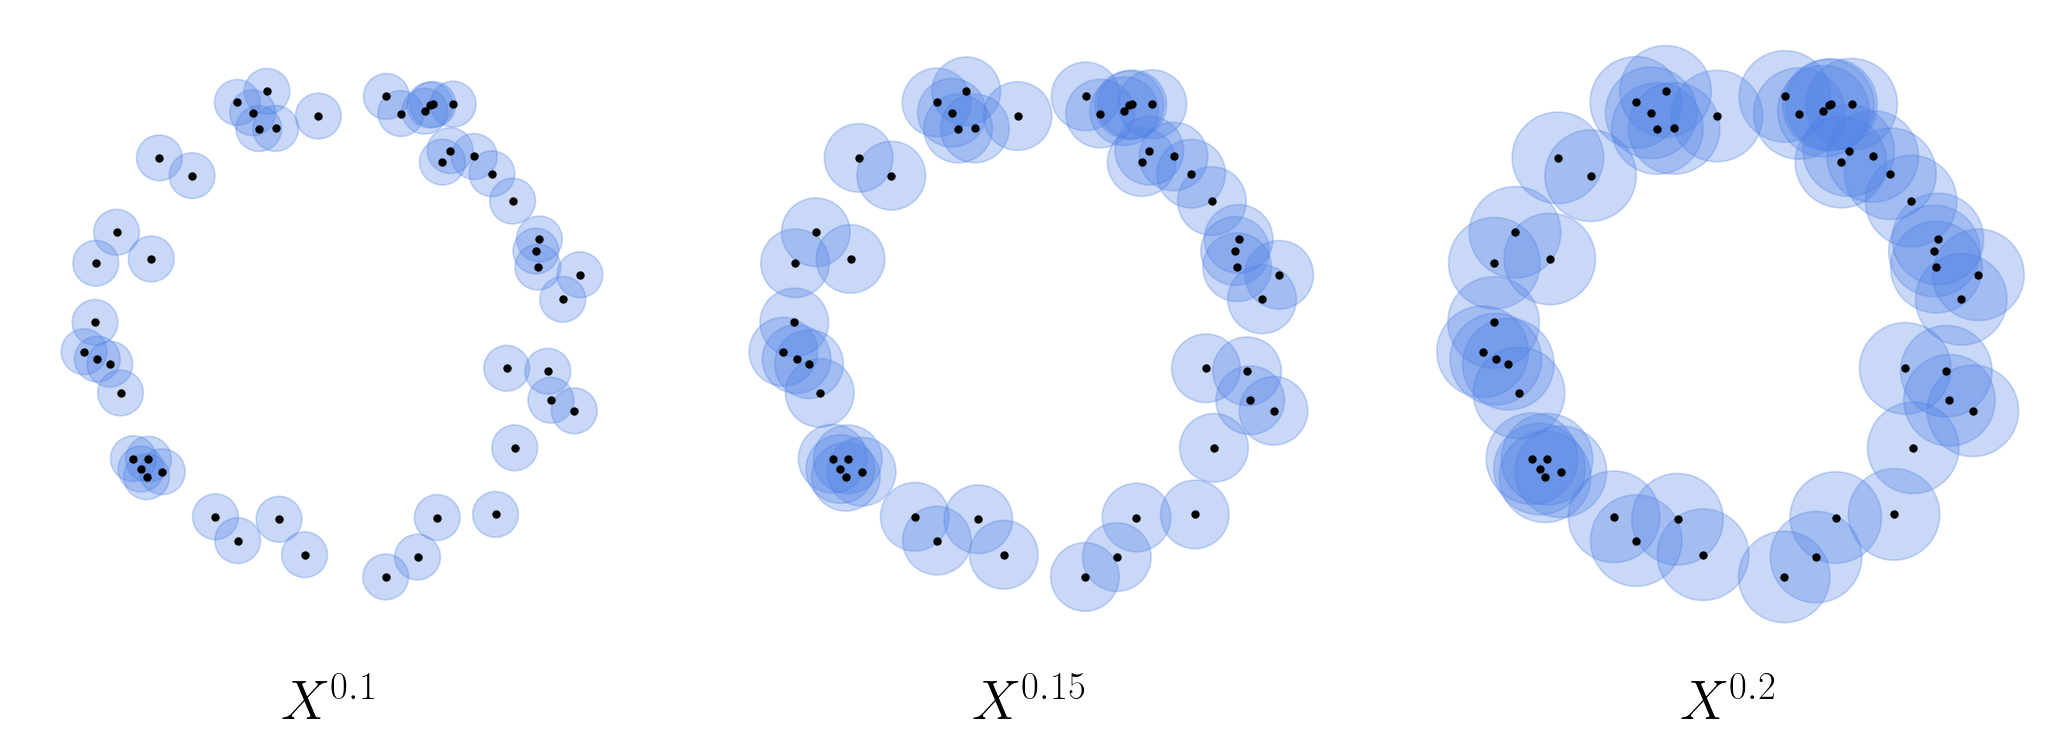
\includegraphics[width=1\textwidth]{Imagens/epessamentos_x.png}
\end{figure}
Observe que a última figura é um espessamento que possui o tipo de homotopia de um círculo: $X^t \approx \mathcal{M}$. Se pudermos selecionar tal $t$, então teremos acesso aos grupos de homologia de $\mathcal{M}$:
\[
    \forall i \geq 0, H_i(\mathcal{M}) \simeq H_i(X).
\]

Se $X \in \mathbb{R}^n$ é um subconjunto finito e $t \geq 0$, queremos calcular o
grupos de homologia $H_0(X^t), \dots ,H_n(X^t)$. Para fazer isso, temos que encontrar uma triangulação de $X^t$, isto é, um complexo simplicial $K$ homeomorfo a $X$. Na verdade, vamos procurar algo um pouco mais fraco: queremos um complexo simplicial $K$ que seja equivalente homotopicamente a $X$.

\ident É fácil representar os espessamentos $X^t$ como complexos simpliciais,
através da noção de coberturas.

\begin{definition}
    Seja $X$ um espçao topológico, uma cobertura de $X$ é a coleção $\mathcal{U} = \left\{U_i\right\}_{1\leq i \leq N}$ do subconjuntos $U_i \subset X$ tal que
    \[
        \bigcup_{1\leq i \leq N} U_i = X.
    \]
\end{definition}
\begin{definition}
    Seja $X$ um espaço topológico e $\mathcal{U} = \{U_i\}_{1 \leq i \leq N}$ uma cobertura de $X$. O nervo de $\mathcal{U}$ é o complexo simplicial com conjunto de vértices $\{1, \ldots, N\}$ cujos $m$-simplexos são os subconjuntos $\{i_1, \ldots, i_m\} \subset \{1, \ldots, N\}$ tais que $\bigcap_{k=0}^{m} U_{i_k} \neq \emptyset$. É denotado $\mathcal{N}(\mathcal{U})$.
    \begin{figure}[H]
        \centering
        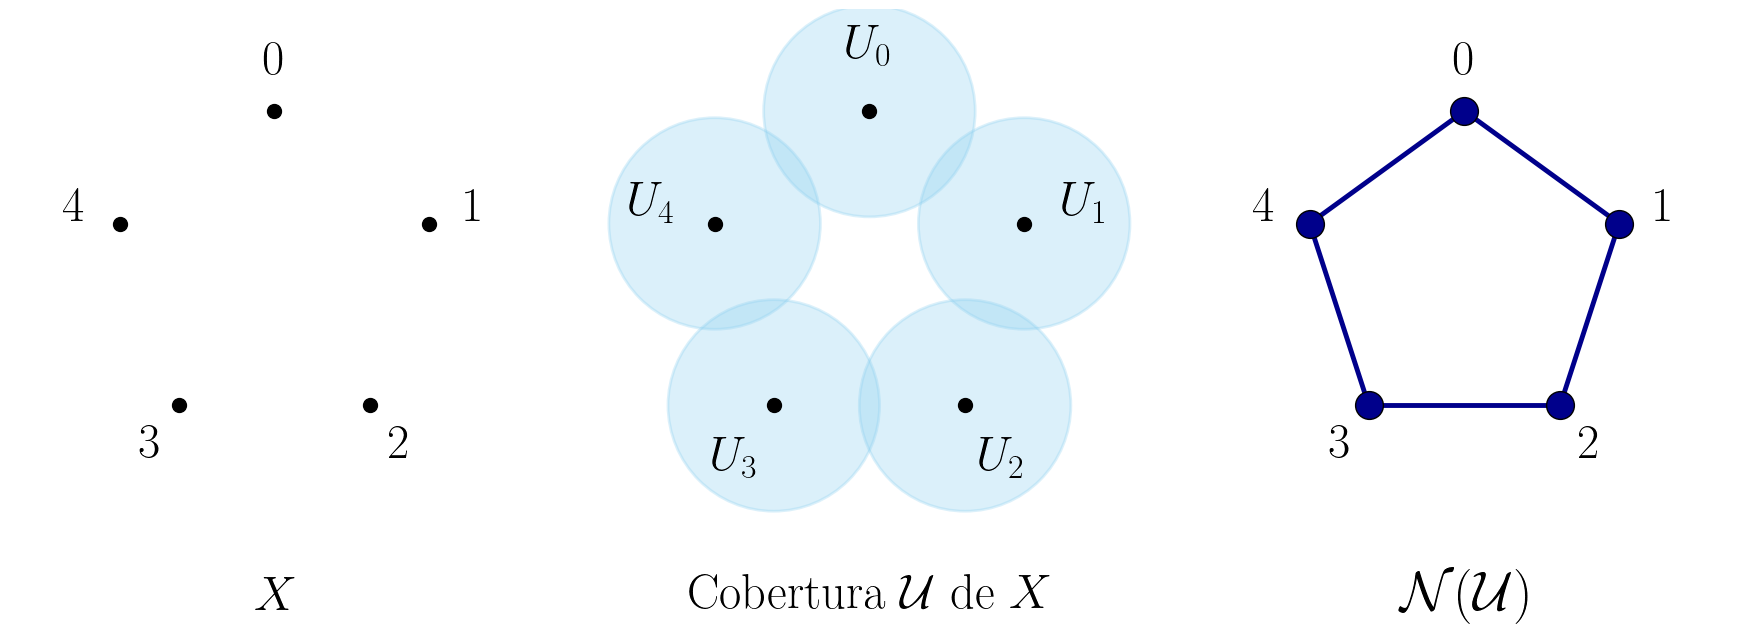
\includegraphics[width=0.8\textwidth]{Imagens/cobertura_nervo.png}
        \caption{Representação da cobertura $\mathcal{U}$ e do nervo $\mathcal{N}(\mathcal{U})$}.
        \label{cobertura_nervo}
    \end{figure}
\end{definition}
\ident Note que a coleção $\mathcal{V}^t=\left\{\overline{\mathcal{B}}(x, t)\mid x \in X\right\}$ é uma cobertura do espessamento $X^t$ e cada componente são bolas fechadas. Consequentemente, podemos considerar seu nervo $\mathcal{N}(\mathcal{V}^t)$. Com isso, segue-se o teorema:

\begin{theorem}
    \hypertarget{teorema_nervo}{}
    Suponha que Y seja um subconjunto de $\mathbb{R}^n$. Considere uma cobertura $\mathcal{U} = \left\{U_i\right\}_{1\leq i \leq N}$ de $Y$ tal que cada um dos $U_i$ são bolas fechadas e convexas. Então $\mathcal{N}(\mathcal{U})$ é homotopia equivalente a Y. (Ver figura \ref{cobertura_nervo}).
\end{theorem}
\vspace{-0.6em}
Demonstração em Tinarrage \cite{tinarrage2021}.

\subsubsection{Complexo de \v{C}ech e de Rips}

\begin{definition}[Complexo de \v{C}ech]
    Sejam $X \subset \mathbb{R}^n$ finito e $t \geq 0$. Considere a coleção $\mathcal{V}^t = \{\overline{\mathcal{B}}(x,t) \mid x \in X\}$. O nervo desta coleção é denotado $\check{\mathrm{C}}\mathrm{ech}^t(X)$ e é chamado de complexo de \v{C}ech de $X$ no instante $t$.
    Explicitamente, $\check{\mathrm{C}}\mathrm{ech}^t(X)$ é o complexo simplicial sobre os vértices $X$ cujos simplexos são os subconjuntos $\{x_{i_1}, \ldots, x_{i_m}\}$ tais que $\bigcap_{k=1}^{m} \overline{\mathcal{B}}(x_{i_k}, t) \neq \emptyset$.
\end{definition}

\ident Como o complexo $\check{\mathrm{C}}\mathrm{ech}^t(X)$ é homotopicamente equivalente ao espessamento $X^t$, o \hyperlink{teorema_nervo}{Teorema do Nervo} garante que os seus respectivos grupos de homologia, $H_i(\check{\mathrm{C}}\mathrm{ech}^t(X))$ e $H_i(X^t)$, são isomorfos. Consequentemente, torna-se viável calcular e acompanhar a evolução da homologia persistente do espessamento computacional $X^t$ por meio do seu equivalente simplicial estruturado.

\ident Embora o complexo de \v{C}ech capture perfeitamente a topologia da união das bolas de raio $t$, a verificação de interseções múltiplas é computacionalmente custosa. Como alternativa tratável, foca-se nas interações aos pares.

\begin{definition}[Complexo de Rips]
    Sejam $X = \{x_1, \ldots, x_N\} \subset \mathbb{R}^n$ um conjunto finito e $t \geq 0$. O complexo de Rips de $X$ no instante $t$, denotado $\mathrm{Rips}^t(X)$, é o complexo do grafo $G^t = \left(\check{\mathrm{C}}\mathrm{ech}^t(X)\right)$ cujo conjunto de vértices é $\{1, \ldots, N\}$ e cujas arestas são os pares $(i,j)$ tais que a distância entre eles obedece a $\|x_i - x_j\| \leq 2t$.

    \begin{figure}[H]
        \centering
        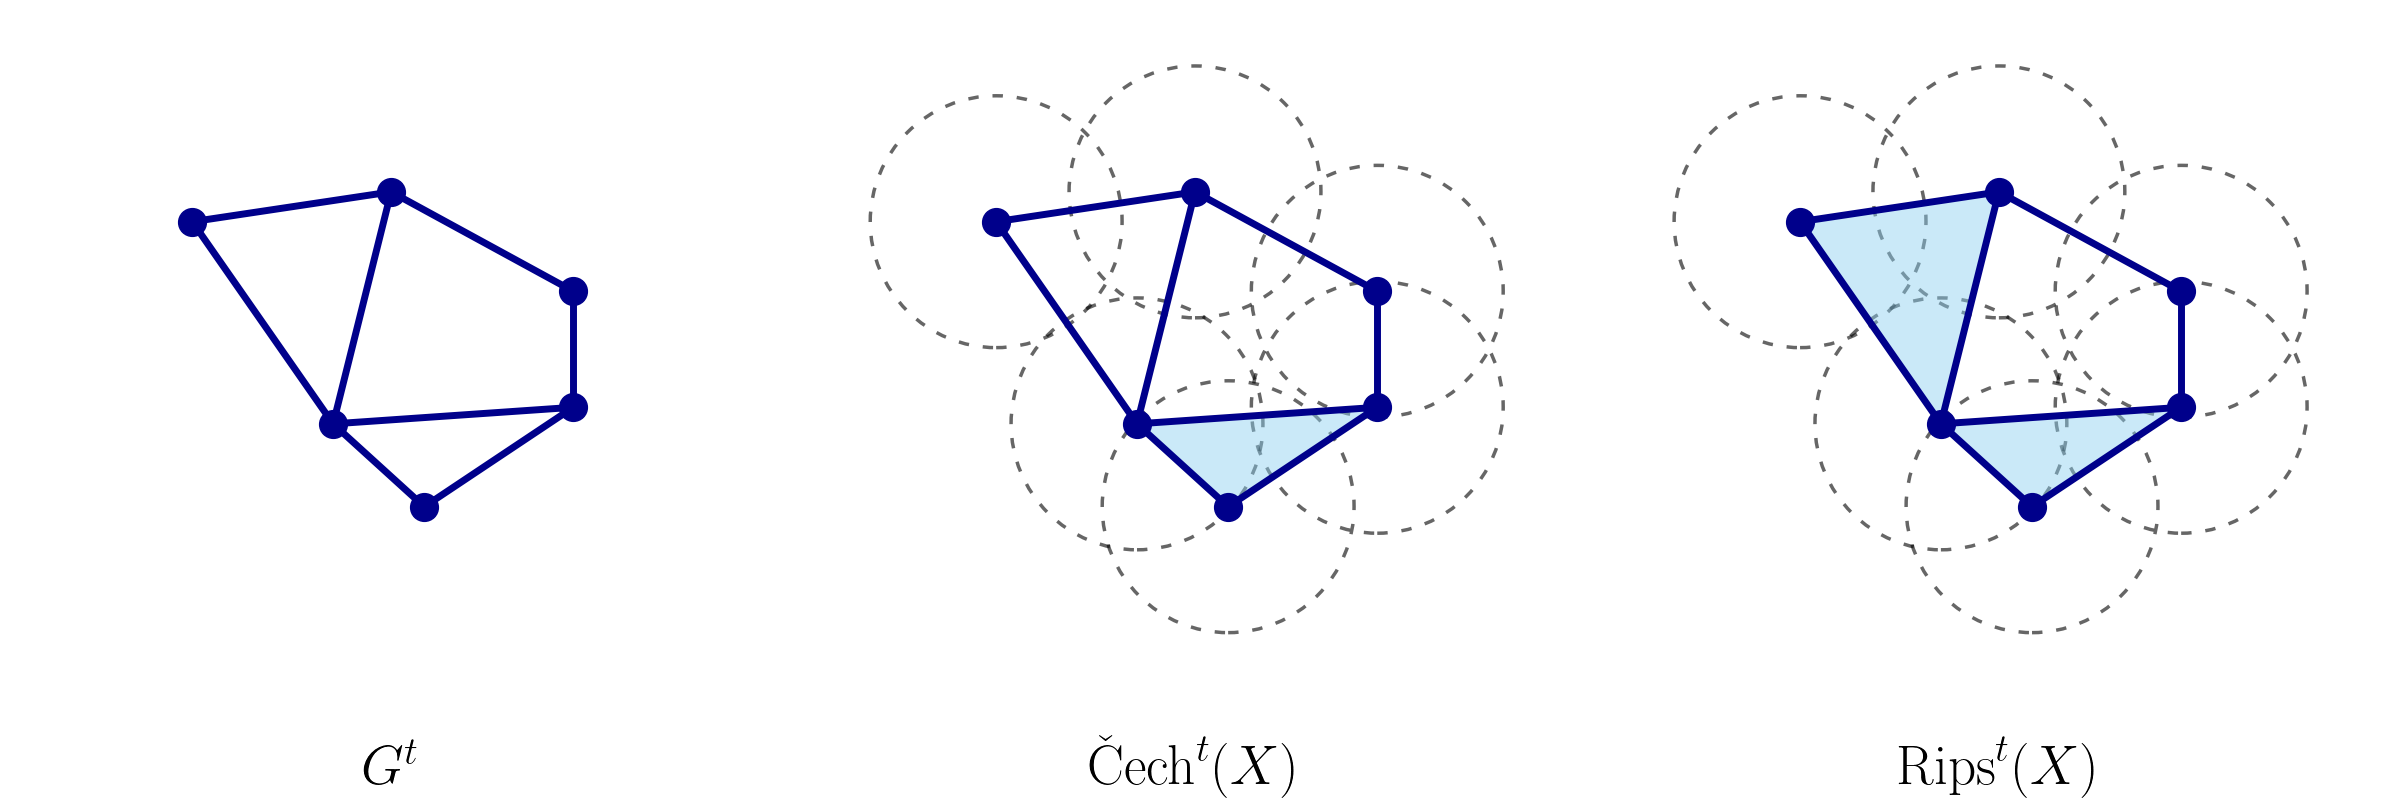
\includegraphics[width=1\textwidth]{Imagens/cech_vs_rips.png}
        \caption{Representação da diferença entre o grafo $G^t$, o complexo de \v{C}ech e o de Rips. Note que o complexo de \v{C}ech só possui 1 simplexo de dimensão 2, pois só há uma interseção entre 3 bolas, já o complexo de Rips, há 2 simplexos de dimensão 2, pois basta que as bolas possuamas interseções dois a dois.}
    \end{figure}
\end{definition}

\ident Observe que o complexo de Rips pode não ser homotopicamente equivalente ao correspondente
Complexo \v{C}ech. No entanto, eles não estão ligados pela seguinte relação:

\begin{proposition}
    Let $X \subset \mathbb{R}^n$ um conjunto finito. Seja $X \subset \mathbb{R}^n$ um subconjunto finito. Para todo $t \geq 0$, temos
    \[
        \textnormal{\v{C}ech}^t(X) \subset \textnormal{Rips}^t(X) \subset \textnormal{\v{C}ech}^{2t}(X).
    \]
\end{proposition}
\vspace{-0.6em}
Demonstração em Tinarrage \cite{tinarrage2021}.

\begin{definition}
    Seja $X \subset \mathbb{R}^n$ e $i\geq 0$. A $i$-ésima curva de Betti de $X$ é a aplicação
    \begin{align*}
        \beta_i(t): \mathbb{R}^+& \longrightarrow \mathbb{N}\\
        &t \longmapsto \beta_i\left(X^t\right)
    \end{align*} 
\end{definition}

A curva de Betti é uma ferramenta ideal para compreender a evolução da homolgia dos complexos simpliciais à medida que $t$ aumenta. Como consequência do \hyperlink{teorema_nervo}{Teorema do Nervo}, a aplicação $t \mapsto \beta_i(t)$ é igual a $t \mapsto \beta_i(\text{\v{C}ech}^t(X))$. Na prática, podemos utilizar a seguinte aplicação, denominada $i$-ésima curva de Betti do complexo de Rips de $X$:
\begin{align*}
    \beta_i^{\textnormal{Rips}}(t): \mathbb{R}^+ &\longrightarrow \mathbb{N}\\
    t &\longmapsto \beta_i\left(\textnormal{Rips}^t(X)\right)
\end{align*}

\begin{example}
    Vejamos uma amostra ruidosa de um circulo $X$
    \begin{figure}[H]
        \centering
        \begin{subfigure}[b]{0.40\textwidth}
            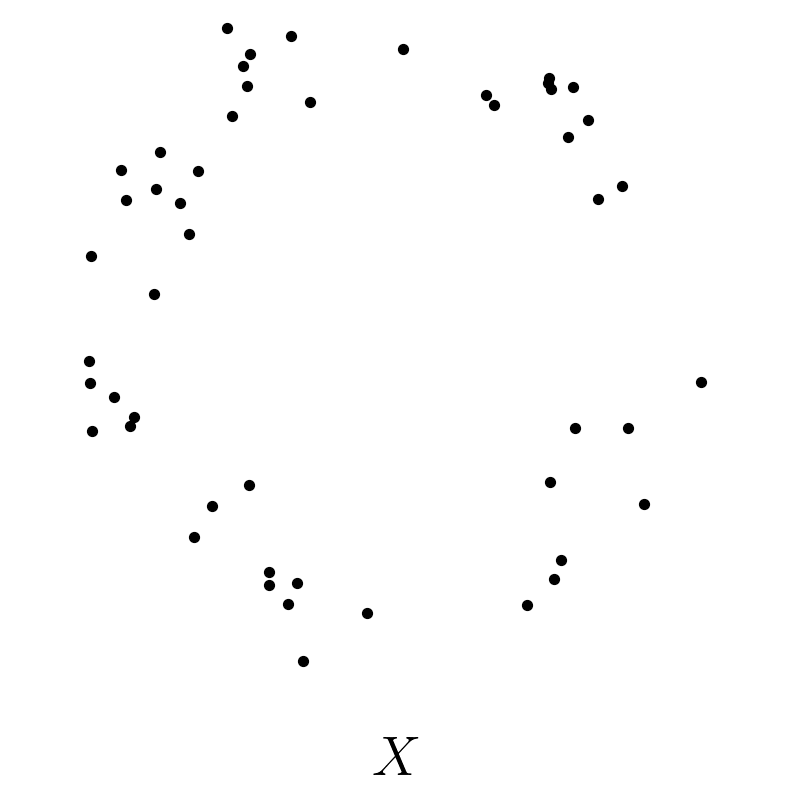
\includegraphics[width=\textwidth]{Imagens/exemplo_curva_betti.png}
        \end{subfigure}
        \hfill
        \begin{subfigure}[b]{0.40\textwidth}
            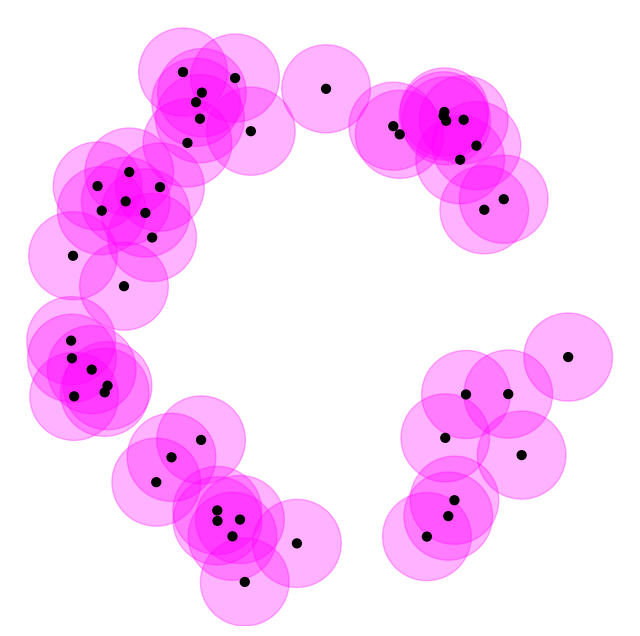
\includegraphics[width=\textwidth]{Imagens/espessamento_betti.png}
        \end{subfigure}
        \hfill
    \end{figure}

    Na figura a direita, podemos observar espessamento de $X$ com $t=0.2$ e disso obtemos que $\beta_0 = 3$, ou seja, 3 componentes conexas e $\beta_1 = 0$. Agora, calculamos as curvas de Betti de $X$.

    \begin{figure}[H]
        \centering
        \begin{subfigure}[b]{0.48\textwidth}
            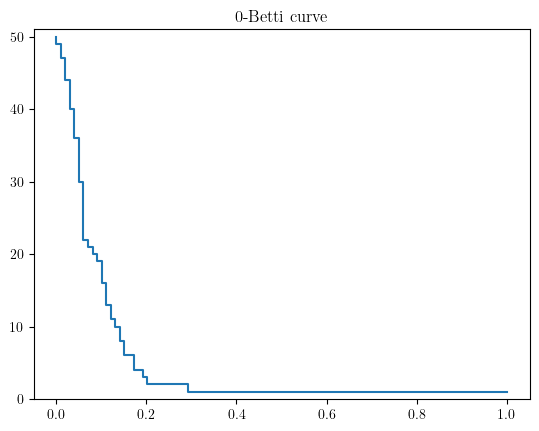
\includegraphics[width=\textwidth]{Imagens/betti0_exemplo.png}
        \end{subfigure}
        \hfill
        \begin{subfigure}[b]{0.48\textwidth}
            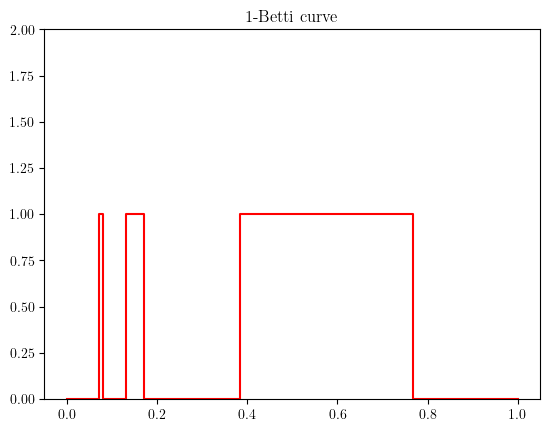
\includegraphics[width=\textwidth]{Imagens/betti1_exemplo.png}
        \end{subfigure}
        \hfill
    \end{figure}

    
\end{example}

\subsection{Módulos de Persistência}
% 
\ident Seja $X \subset \mathbb{R}^n$ uma nuvem de pontos finita amostrada de um objeto topológico subjacente $\mathcal{M}$. Para inferir a forma de $\mathcal{M}$, construímos aproximações geométricas, como os complexos de \v{C}ech $\check{C}_t(X)$ ou de Rips $R_t(X)$, baseados em um parâmetro de escala (ou espessamento) $t \geq 0$. Na prática, a escolha de um limiar $t$ estático é extremamente crítica e instável: as curvas dos números de Betti $t \mapsto \beta_i(X_t)$ assumem apenas valores inteiros e são descontínuas. Além disso, as nuvens de pontos reais sofrem de ``ruído topológico'', caracterizado por pequenos ciclos geométricos que surgem e desaparecem abruptamente.

\ident Para extrair a verdadeira homologia de $\mathcal{M}$ e ignorar o ruído, a Homologia Persistente adota uma mudança de paradigma: em vez de tentar adivinhar um único $t$ ótimo, analisamos todos os espessamentos simultaneamente. Observando a evolução de toda a família de complexos filtrados, conseguimos rastrear quais buracos são persistentes (a verdadeira forma) e quais são efêmeros (ruído). O rigor matemático que permite rastrear esses ciclos ao longo do tempo repousa sobre uma propriedade fundamental da homologia: a sua functorialidade.

\ident Na Teoria das Categorias, um functor é essencialmente um ``dicionário'' que traduz de forma consistente objetos e morfismos de uma categoria matemática para outra, preservando a sua estrutura relacional. É esta aplicação linear induzida que nos diz a localização de um ciclo topológico quando o complexo cresceu. Para formalizarmos como a functorialidade opera computacionalmente, precisamos estudá-la sob uma perspectiva discreta. Introduzimos a seguir a definição de aplicação simplicial, que atua como a contraparte geométrica das aplicações contínuas.

\begin{definition}
    Sejam $K$ e $L$ dois complexos simpliciais, e $V_K, V_L$ seus conjuntos de vértices. Uma aplicação simplicial entre $K$ e $L$ é uma aplicação $f: V_K \to V_L$ tal que
    \[
    \forall \sigma \in K, f(\sigma) \in L.
    \] 
    Quando não houver risco de confusão, podemos denotar uma aplicação simplicial como $f: K \to L$ em vez de $f: V_K \to V_L$.
\end{definition}

\begin{example}
    Sejam $K = \{[0], [1], [0, 1]\}, L = \{[0], [1], [2], [0, 1], [0, 2], [1, 2]\}$ e $f : \{0, 1\} \to\{0, 1, 2\}$ definida por $f(0) = 0$ e $f(1) = 1$. Ela é uma aplicação simplicial, uma vez que $f([0, 1]) = [0, 1]$ é um
    simplexo de $L$.
\end{example}
    
\begin{example}
    Sejam $K = \{[0], [1], [2], [0, 1], [0, 2], [1, 2]\}, L = \{[0], [1], [2], [0, 1], [0, 2]\}$ e $f : \{0, 1, 2\} \to\{0, 1, 2\}$ definida por $f(0) = 0$, $f(1) = 1$ e $f(2) = 2$. Ela não é uma aplicação simplicial, uma vez que $f([1, 2]) = [1, 2]$ não é um
    simplexo de $L$.
\end{example}

\begin{definition}
    Seja $f:K\to L$ uma aplicação simplicial. Seja $n\geq0$, e considerando os grupos de cadeias $K$ e $L$:
    \begin{align*}
        C_n(K) &= \left\{\sum_{\sigma \in K_{(n)}} \epsilon_\sigma \cdot \sigma \mid \forall\sigma \in  K_{(n)}, \, \epsilon_\sigma \in \mathbb{Z}/2/\mathbb{Z}  \right\}\\
        C_n(L) &= \left\{\sum_{\sigma \in L_{(n)}} \epsilon_\sigma \cdot \sigma \mid \forall\sigma \in  K_{(n)}, \, \epsilon_\sigma \in \mathbb{Z}/2/\mathbb{Z}  \right\}
    \end{align*}
    Definimos uma aplicação linear $f_n: C_n(K) \to C_n(L)$ da seguinte forma:
    \[
    f_n (\sigma) =
    \begin{cases}
        f(\sigma) \quad, \textnormal{se} \,\, \dim (f(\sigma)) = n,\\
        0 \quad\quad\,\,\,, \textnormal{caso contrário}.
    \end{cases}
    \]
\end{definition}

\begin{proposition}
    Para todo $c \in Z_n(K)$ e $b \in B_n(K)$, tem-se $f_n(c) \in Z_n(L)$ e $f_n(b) \in
Bn(L)$.

Esta proposição nos diz que, a imagem de um ciclo é um ciclo e a imagem de fronteira é uma fronteira.
\end{proposition}
\vspace{-0.6em}
Demonstração em Tinarrage \cite{tinarrage2021}.

Lembremos que $B_n(K) \subset Z_n(K)$ e $B_n(L) \subset Z_n(L)$. A proposição anterior mostra que a aplicação $f_n$ induz uma aplicação linear entre
espaços vetoriais quociente:
\begin{align*}
    (f_n)_* : Z_n(K)/B_n(K) \longrightarrow Z_n(L)/B_n(L).
\end{align*}
Pela definição dos grupos de homologia, definimos uma aplicação linear
\begin{align*}
    (f_n)_* : H_n(K) \longrightarrow H_n(L).
\end{align*}
Ela é chamada de aplicação induzida na homologia. Podemos denotá-lo, também, por $f_*$ em vez de $(f_n)_*$. Explicitamente, a aplicação $(f_n)_*$ pode ser descrito da seguinte forma:
\[
c = \sum_{\sigma \in K(n)} \epsilon_\sigma \cdot \sigma \longmapsto \sum_{\sigma \in K(n)} \epsilon_\sigma \cdot f_n(\sigma)
\]

\begin{definition}
    Uma filtração de um complexo simplicial é uma família de subconjuntos $\mathbb{X} = (X^t)_{t \in \mathbb{R}^+}$ de $E$ é uma filtração se for não decrescente em relação à inclusão; isto é, para quaisquer $s, t \in \mathbb{R}^+$, se $s \leq t$, então $X_s \subseteq X_t$.
\end{definition}

\ident Seja $X \subset \mathbb{R}^n$. A coleção de seus espessamentos é uma sequência não decrescente de subconjuntos
\[
    \dots \subset X^{t_1} \subset X^{t_2} \subset X^{t_3} \subset \dots
\]
Ao considerar os complexos de Rips correspondentes, obtemos uma sequência não decrescente de complexos simpliciais
\[
    \dots \subset \textnormal{Rips}^{t_1}(X) \subset \textnormal{Rips}^{t_2}(X) \subset \textnormal{Rips}^{t_3}(X) \subset \dots
\]
Denotemos por $i_s^t$ a aplicação de inclusão correspondente a $\textnormal{Rips}^s(X) \subset \textnormal{Rips}^t(X)$. Podemos escrever
\begin{align*}
    \dots \longrightarrow \textnormal{Rips}^{t_1}(X) \xrightarrow{\quad i_{t1}^{t2} \quad} \textnormal{Rips}^{t_2}(X) \xrightarrow{\quad i_{t2}^{t3} \quad} \textnormal{Rips}^{t_3}(X) \longrightarrow \dots
\end{align*}
A aplicação do functor de homologia de ordem $i$ resulta em um diagrama de espaços vetoriais
\begin{align*}
    \dots \rightarrow H_i\left(\textnormal{Rips}^{t_1}(X)\right) \xrightarrow{\quad \left(i_{t1}^{t2}\right)_* \quad} H_i\left(\textnormal{Rips}^{t_2}(X)\right) \xrightarrow{\quad \left(i_{t2}^{t3}\right)_* \quad} H_i\left(\textnormal{Rips}^{t_3}(X)\right) \rightarrow \dots
\end{align*}
onde as aplicaçãoes $(i_s^t)_*$ são aquelas induzidas na homologia pelas inclusões $i_s^t$. Nessa sequência,podemos observar por quanto tempo um ciclo vive, ou persiste. Sejam $i \geq 0$, $t_0 \geq 0$ e considere um
ciclo $c \in H_i(\textnormal{Rips}^{t_0}(X))$. Seu tempo de morte é
\begin{align*}
    \sup \{t \geq t_0, \left(i^t_{t0}\right)(c)\neq 0\}
\end{align*}
e seu tempo de nascimento é
\begin{align*}
    \inf \{t \geq t_0, \left(i^t_{t0}\right)^{-1}(\{c\})\neq \emptyset\}.
\end{align*}

Medimos a persistência de $c$ como a diferença entre seu instante de morte e seu instante de nascimento. Como regra geral, espera-se que ciclos com alta persistência correspondam a características topológicas importantes do conjunto de dados, e que ciclos com baixa persistência
correspondam a ruído topológico.

\begin{definition}
    Um módulo de persistência $\mathbb{V}$ sobre $\mathbb{R}^+$ com coeficientes em $\mathbb{Z}/2\mathbb{Z}$ é um par $(\mathbb{V}, v)$ onde: $\mathbb{V} = (V^t)_{t \in \mathbb{R}^+}$ é uma família de $\mathbb{Z}/2\mathbb{Z}$-espaços vetoriais, $\mathbbm{v} = (v_s^t: V^s \to V^t)_{s \leq t \in \mathbb{R}^+}$ é uma família de aplicaçãoes lineares tais que:
    \begin{itemize}
        \item para todo $t \in \mathbb{R}^+$, a aplicação $v_t^t: V^t \to V^t$ é a identidade,
        \item para todo $r,s,t \in \mathbb{R}^+$ tais que $r \leq s \leq t \in \mathbb{R}^+$, temos $v_s^t \circ v_r^s = v_r^t$.
    \end{itemize}
\end{definition}

\begin{definition}
    Um isomorfismo entre dois módulos de persistência $\mathbb{V}$ e $\mathbb{W}$ é uma família de isomorfismos de espaços vetoriais $\phi = (\phi_t: V^t \to W^t)_{t \in \mathbb{R}^+}$ tal que o seguinte diagrama comuta para todo $s \leq t \in \mathbb{R}^+$:
    \[
        \begin{array}{ccc}
        V^s & \xrightarrow{v_s^t} & V^t \\
        \downarrow_{\phi_s} & & \downarrow_{\phi_t} \\
        W^s & \xrightarrow{w_s^t} & W^t
        \end{array}
    \]
\end{definition}

\begin{definition}
    Seja $\mathbb{V}, \mathbbm{v}$ e $\mathbb{W}, \mathbbm{w}$ dois módulos de persistência. A soma de dois módulos de persistência $\mathbb{V} \oplus \mathbb{W}$ definidos pelos espaços vetoriais $\left(V \oplus W\right)^t=V^t\oplus W^t$ e as aplicações lineares
    \begin{align*}
        (v\oplus w)_s^t:(x,y) \in \left(V \oplus W\right)^s \longmapsto (v_s^t(x), w_s^t(y)) \in \left(V \oplus W\right)^t
    \end{align*}

\end{definition}

\begin{definition}
    Seja $I \subset \mathbb{R}^+$ um intervalo (conjunto convexo não-vazio). O módulo intervalar associado a $I$, denotado $\mathbb{B}[I]$, é o módulo de persistência com espaços vetoriais e aplicações lineares definidos por:
    \[
        \mathbb{B}^t[I] = \begin{cases} \mathbb{Z}/2\mathbb{Z} & \textnormal{se } t \in I, \\ 0 & \textnormal{caso contrário,} \end{cases}
        \quad \textnormal{e} \quad
        v_s^t = \begin{cases} \mathrm{id} & \textnormal{se } s, t \in I, \\ 0 & \textnormal{caso contrário.} \end{cases}
    \]
\end{definition}

\begin{definition}
    Um módulo de persistência $\mathbb{U}$ é indecomponível se, para todo par de módulos de persistência $\mathbb{V}$ e $\mathbb{W}$ tais que $\mathbb{U} \simeq \mathbb{V} \oplus \mathbb{W}$, um dos somandos é o módulo trivial (identicamente nulo). Caso contrário, $\mathbb{U}$ é decomponível.

    Um módulo de persistência $\mathbb{V}$ é dito decomponível em módulos intervalares se existe um multiconjunto $\mathcal{I}$ de intervalos de $\mathbb{R}^+$ tal que:
    \[
        \mathbb{V} \simeq \bigoplus_{I \in \mathcal{I}} \mathbb{B}[I].
    \]
    O termo \enquote{multiconjunto} significa que $\mathcal{I}$ pode conter várias cópias do mesmo intervalo $I$. Diz-se que tal módulo é decomponível em módulos intervalares, ou simplesmente decomponível, quando o contexto estiver claro.
\end{definition}

\begin{theorem}
    Se um módulo de persistência $\mathbb{V}$ se decompõe em módulos intervalares, então o multiconjunto $\mathcal{I}$ de intervalos é único. Além disso, se todos espaços vetoriais $V^t$ de $\mathbb{V}$ tiverem dimensão finita, entãao $V$ se decompõe em módulos intervalares.
\end{theorem}

Nesse caso, $\mathcal{I}$ é chamado de código de barras de persistência de $\mathbb{V}$, ou simplesmente código de barras (\textit{barcode}). Escreve-se $\textnormal{Barcode}\left(\mathbb{V}\right)$.

\begin{definition}
    Seja $\mathrm{Barcode}(\mathbb{V})$ o barcode de um módulo decomponível. Para cada intervalo $[a,b]$, $(a,b]$, $[a,b)$ ou $(a,b)$ no $\mathrm{Barcode}(\mathbb{V})$, com pontencialmente $a = -\infty$ ou $b = \infty$, considere-se o ponto $(a,b) \in \mathbb{R}^2$. A coleção de todos estes pontos forma o multiconjunto chamado diagrama de persistência, denotado $\mathrm{Diagram}(\mathbb{V})$.

    \begin{figure}[H]
        \centering
        \begin{subfigure}[b]{0.24\textwidth}
            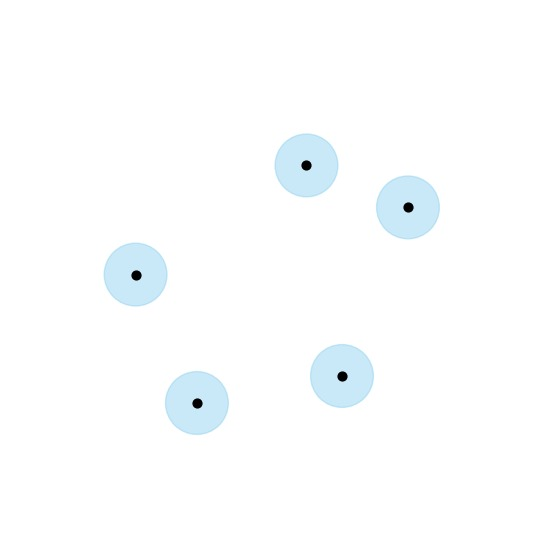
\includegraphics[width=\textwidth]{Imagens/barcode_simplexo_0.5.png}
        \end{subfigure}
        \hfill
        \begin{subfigure}[b]{0.24\textwidth}
            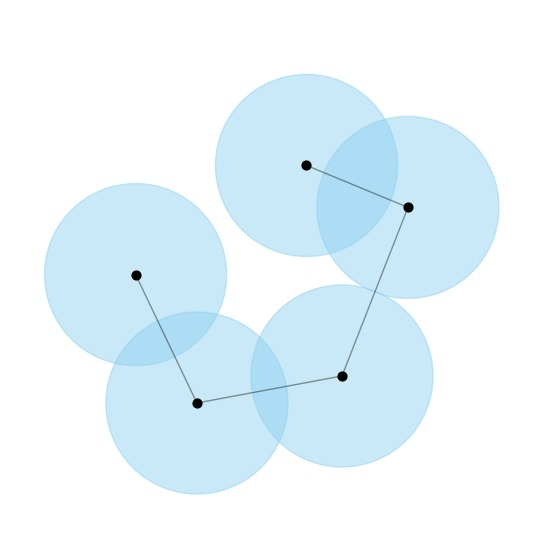
\includegraphics[width=\textwidth]{Imagens/barcode_simplexo_1.45.png}
        \end{subfigure}
        \hfill
        \begin{subfigure}[b]{0.24\textwidth}
            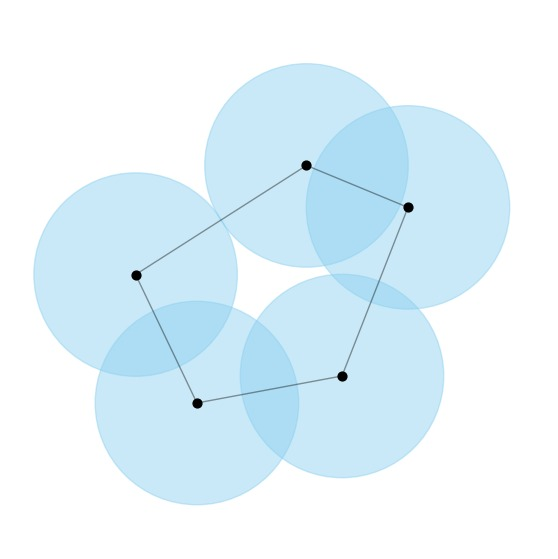
\includegraphics[width=\textwidth]{Imagens/barcode_simplexo_1.62.png}
        \end{subfigure}
        \hfill
        \begin{subfigure}[b]{0.24\textwidth}
            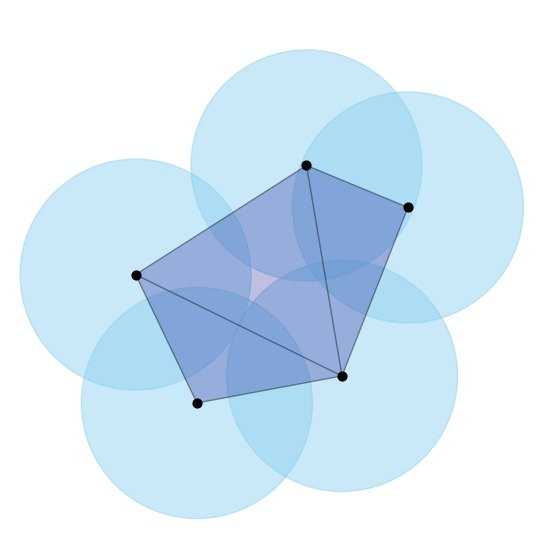
\includegraphics[width=\textwidth]{Imagens/barcode_simplexo_1.84.png}
        \end{subfigure}

        \vspace{0.5cm}

        \begin{subfigure}[b]{0.48\textwidth}
            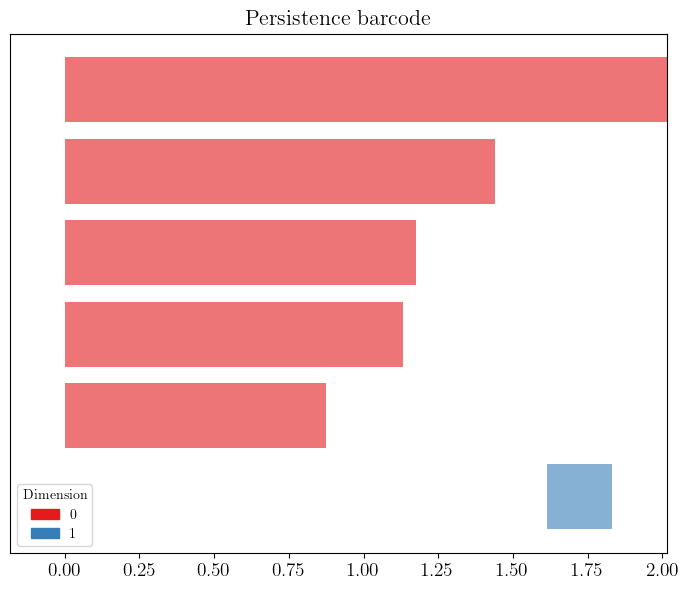
\includegraphics[width=\textwidth]{Imagens/barocode_def.png}
        \end{subfigure}
        \hfill
        \begin{subfigure}[b]{0.48\textwidth}
            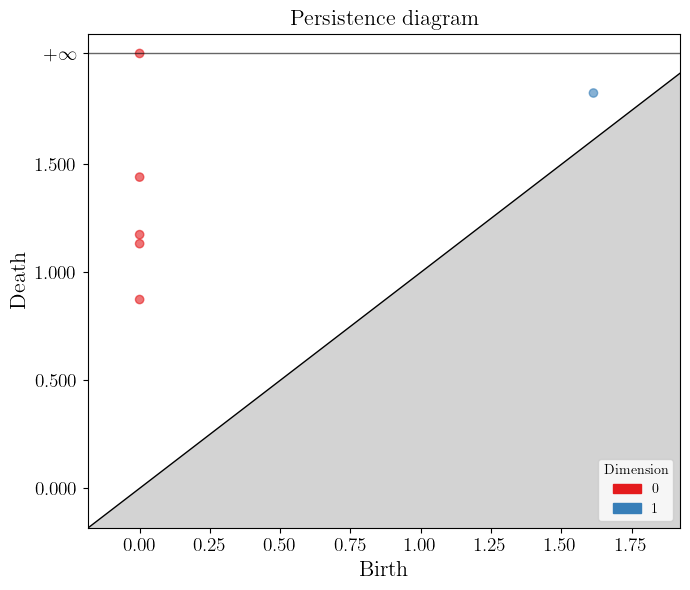
\includegraphics[width=\textwidth]{Imagens/diagrama_def.png}
        \end{subfigure}

    \caption{Acima vemos um complexo de Rips em 4 instantes: $d=0.5$, $d=1.45$, $d=1.62$ e $d=1.84$. Abaixo segue-se com o \textit{Persistence Barcode} gerado a partir da filtração de Vietoris-Rips. Cada linha horizontal representa a duração de uma característica homológica através das escalas de filtração, evidenciando as componentes conexas em dimensão 0 e a assinatura persistente do ciclo em dimensão 1. E o Diagrama de Persistência mapeando os pares de nascimento e morte das feições topológicas. O ponto vermelho afastado da diagonal principal indica o ciclo gerador persistente de dimensão 1. Podemos realizar a relação instante do complexo com o seu \textit{Barcode} e seu Diagrama de Persistência.}
    \end{figure}
\end{definition}

\subsection{Paisagens de Persitência}\label{sec:paisagens_persitencia}
\ident Embora os Diagramas de Persistência resumam o ciclo de vida das classes de homologia (nascimento $b$ e morte $d$), eles habitam um espaço métrico não-linear. Para que possamos calcular médias, variâncias e aplicar algoritmos de aprendizado de máquina diretamente nestes invariantes, utilizamos a vetorização contínua idealizada por Bubenik \cite{Bubenik2015}.

\begin{definition}\label{paisagem_persistencia_def}
    Dado um diagrama de persistência com intervalos $\mathcal{B} = \{(b_i, d_i)\}_{i=1}^m$, define-se para cada ponto a função auxiliar:
    \[
        f_{(b,d)}(t) = \max(0, \min(t-b,\; d-t)).
    \]
    A paisagem de persistência é a sequência de funções $\lambda_k : \mathbb{R} \to \mathbb{R}$ definidas por:
    \[
        \lambda_k(t) = k\text{-ésimo maior valor do conjunto } \{f_{(b_i,d_i)}(t)\}_{i=1}^m,
    \]
    adotando $\lambda_k(t) = 0$ caso $k > m$.
\end{definition}

\begin{figure}[H]
    \centering
    % --- linha 1: barcode + diagrama ---
    \begin{subfigure}[b]{0.48\textwidth}
        \centering
        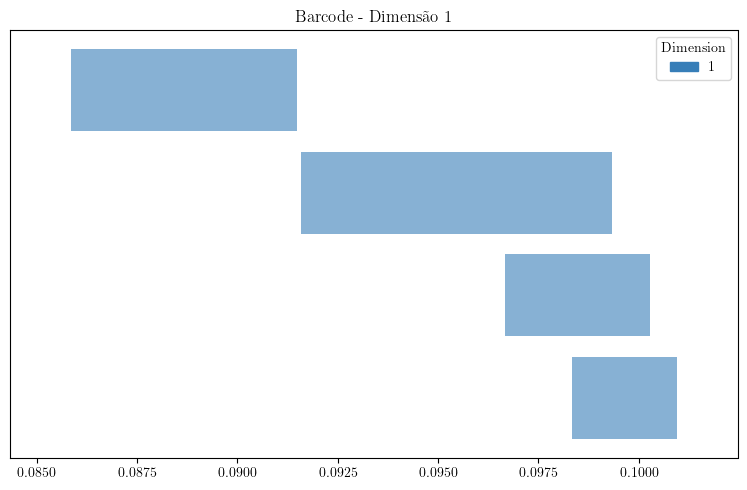
\includegraphics[width=\linewidth]{Imagens/barcode_landscape.png}
        \caption{Barcode ($H_1$)}
        \label{fig:barcode}
    \end{subfigure}
    \hfill
    \begin{subfigure}[b]{0.48\textwidth}
        \centering
        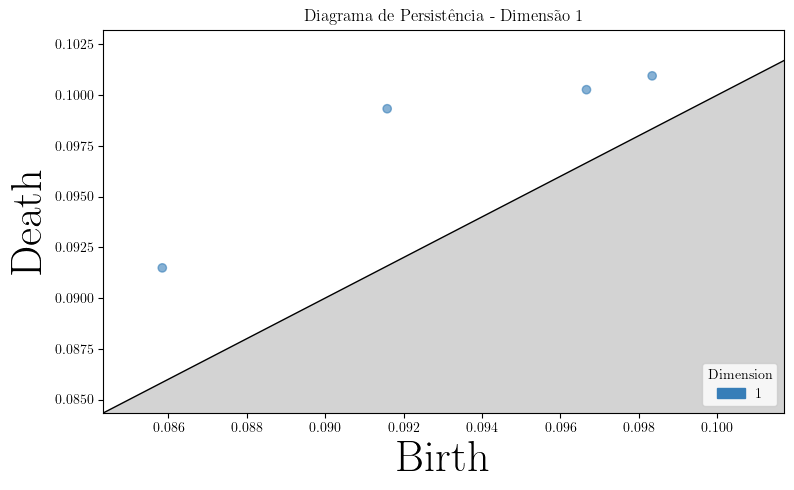
\includegraphics[width=\linewidth]{Imagens/diagrama_landscape.png}
        \caption{Diagrama de persistência}
        \label{fig:diagrama}
    \end{subfigure}
    
    \vspace{0.9em}

    \begin{subfigure}[b]{0.48\textwidth}
        \centering
        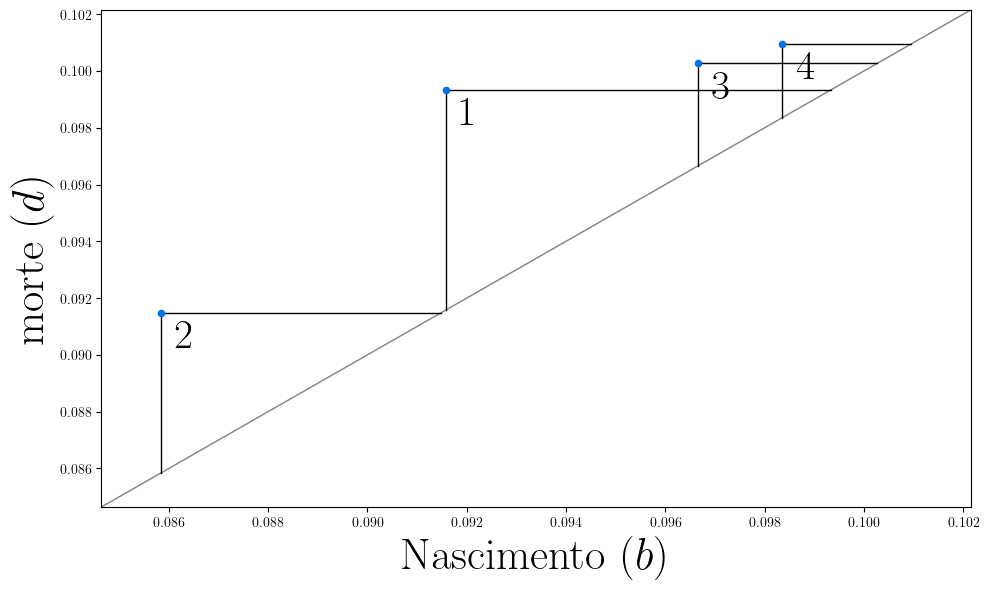
\includegraphics[width=\linewidth]{Imagens/triangulacao_diagrama.png}
            \caption{Diagrama triangulado}
        \label{fig:diagrama_triangulado}
    \end{subfigure}
    \hfill
    \begin{subfigure}[b]{0.48\textwidth}
        \centering
        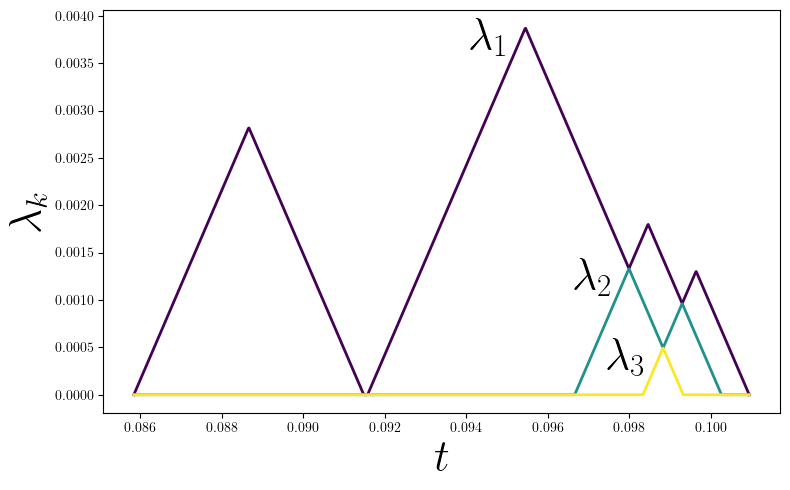
\includegraphics[width=\linewidth]{Imagens/landscapes_2d.png}
        \caption{Landscape (2D)}
        \label{fig:landscape2d}
    \end{subfigure}

    \vspace{0.5em}
% \end{figure}

% \begin{figure}[H]
    % \ContinuedFloat
    \centering

    % --- linha 3: landscape 3D ---
    \begin{subfigure}[b]{0.7\textwidth}
        \centering
        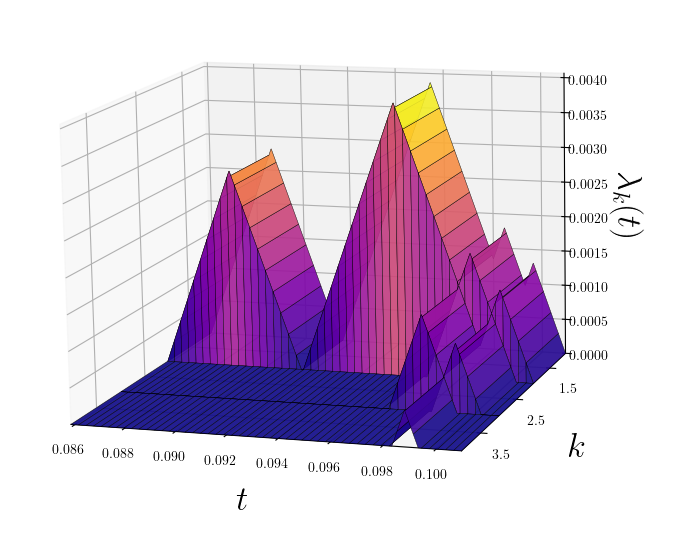
\includegraphics[width=\linewidth]{Imagens/landscapes_3d.png}
        \caption{Landscape (3D)}
        \label{fig:landscape3d}
    \end{subfigure}

    % Legenda completa e final com o rótulo principal
    \caption{Construção da paisagem de persistência (continuação). 
    (a)–(b) Barcode e diagrama de persistência padrão para $H_1$. (c) O mesmo diagrama com os triângulos de cada ponto $(b,d)$ explicitados: a perna vertical (nascimento) e a horizontal (morte) ligam o ponto à diagonal. (d) Cada triângulo de (c) corresponde a uma \enquote{tenda} $f_i(t)=\max(0,\min(t-b_i,\,d_i-t))$; a landscape $\lambda_k(t)$ é o $k$-ésimo maior valor dessas tendas em cada $t$, plotada aqui camada a camada. (e) As mesmas camadas $\lambda_k$, agora dispostas como um relevo tridimensional $(t, k, \lambda_k(t))$, evidenciando a estrutura de múltiplas camadas da landscape do complexo.}
    \label{fig:pipeline_landscape}
\end{figure}

\begin{definition}
    Sejam $\lambda (k,t)$ e $\lambda '(k,t)$ duas paisagens paisagens de persistências. A distância topológica (distância $p$-Paisagem) entre duas paisagens $\lambda$ e $\lambda'$ é dada pela norma em espaços de Banach $L^p$:
    \begin{equation*}
        \Lambda_p(\lambda, \lambda') = \|\lambda - \lambda'\|_p = \left( \sum_{k=1}^\infty \int_{\mathbb{R}} |\lambda_k(t) - \lambda'_k(t)|^p \, dt \right)^{1/p}.
    \end{equation*}
\end{definition}

\ident O corolário analítico mais profundo advindo da formulação das Paisagens de Persistência reside no fato de que a função $\lambda_k(t)$ é, por definição, um elemento do espaço integrável de Lebesgue $L^p(\mathbb{N} \times \mathbb{R})$. Uma vez que o espaço $L^p$ detém a estrutura de um Espaço de Banach, caracterizando-se como um espaço vetorial normado e completo, as barreiras algébricas inerentes aos diagramas de persistência não-lineares são superadas. A existência de um Espaço de Hilbert é de suma importância para a modelagem estatística, pois assegura a formulação rigorosa de um produto interno $\langle \lambda, \lambda' \rangle_{L^2}$. Consequentemente, a aplicabilidade do Teorema de Representação de Riesz fica matematicamente garantida, assegurando que qualquer funcional linear contínuo sobre este espaço funcional possa ser perfeitamente representado através deste produto interno. É precisamente esta transição exata, da combinatória abstrata dos complexos simpliciais para a continuidade analítica em espaços de Hilbert, que legitima o uso do Teorema de Mercer. Ao garantir a existência de uma função de \textit{kernel} simétrica e definida positiva associada a esse produto interno, o espaço de Hilbert viabiliza a utilização do método das Máquinas de Vetores de Suporte (que irá ser abordado na subseção \ref{secao_svm}), provendo a base teórica para o cálculo do hiperplano ótimo de separação entre os estados dinâmicos da proteína.

\section{Inferência Estatística sobre Invariantes Topológicos}

\ident O desenvolvimento da Homologia Persistente e, em particular, das Paisagens de Persistência, forneceu-nos um espaço funcional contínuo para representar os dados. No entanto, o objetivo fundamental deste trabalho exige que avaliemos, com significância estatística, se a dinâmica estrutural da proteína MBP no seu estado \textit{Apo} (aberta) diverge da sua dinâmica no estado \textit{Holo} (fechada). Para tal, é necessário traduzir o espaço de Banach num domínio probabilístico clássico \cite{devore2012}.

\subsection{A Variável Aleatória Topológica}

\ident A fim de aplicar os métodos de inferência estatística tradicional, precisamos de reduzir a representação funcional da topologia a um escalar real que capture a magnitude global da persistência \cite{kovacev2016}. 

\ident Seja $\lambda_k(t)$ a $k$-ésima função da paisagem de persistência gerada a partir da matriz de distâncias dinâmicas de uma dada conformação proteica. Definimos uma variável aleatória contínua $X$ como a área total sob todas as curvas da paisagem de persistência:
\begin{equation}
    X = \sum_{k=1}^{\infty} \int_{\mathbb{R}} \lambda_k(t) \, dt
\end{equation}

\ident Ao integrarmos as funções de paisagem no domínio real, a variável $X$ corresponde à área total abrangida por todos os contornos $\lambda(k, t)$, $k \in \mathbb{N}$, de uma paisagem de persistência. \cite{Bubenik2015}. Como as flutuações atómicas oriundas do Modelo de Rede Anisotrópica (ANM) possuem natureza estocástica, a paisagem gerada por cada amostra proteica é, consequentemente, uma realização empírica de um processo estocástico. Assim, $X$ herda as propriedades de uma variável aleatória com uma distribuição de probabilidade subjacente (e desconhecida) com esperança matemática $\mu$ e variância $\sigma^2$ \cite{devore2012}.

\subsection{Formulação das Hipóteses}

\ident Consideremos duas populações teóricas independentes: a população das conformações fechadas da MBP, cuja variável aleatória topológica denotaremos por $X_1$ (com média $\mu_1$), e a população das conformações abertas, denotada por $X_2$ (com média $\mu_2$). 

\ident O nosso objetivo é determinar se a diferença observada nas áreas das paisagens de persistência entre os dois grupos reflete uma verdadeira divergência na dinâmica biomolecular ou se resulta de mero ruído amostral. Formulamos, assim, o seguinte teste de hipóteses \cite{kovacev2016}:
\begin{align*}
    H_0 &: \mu_1 = \mu_2 \quad \left(\parbox{7.5cm}{A hipótese nula: as topologias médias são idênticas}\right) \\[0.5em]
    H_a &: \mu_1 \neq \mu_2 \quad \left(\parbox{7.5cm}{A hipótese alternativa: as topologias médias diferem significativamente}\right)
\end{align*}

\ident Devido à estrutura do espaço de Banach, a variável $X$ satisfaz a Lei dos Grandes Números e o Teorema Central do Limite \cite{Bubenik2015}. Isso implica que, para uma amostra suficientemente grande ($n \to \infty$), a distribuição da média amostral $\overline{X}$ aproximar-se-ia de uma distribuição Normal. Contudo, em contextos biológicos e cristalográficos, o número de estruturas resolvidas com alta qualidade é frequentemente limitado. 

\subsection{O Teste de Permutação Não-Paramétrico}

\ident No estudo de Kovacev-Nikolic et al. (2016), a amostra disponível continha apenas $n = 14$ estruturas de MBP (sendo sete na forma aberta e sete na fechada) \cite{kovacev2016}. Com amostras tão diminutas, a suposição de normalidade exigida por testes paramétricos clássicos (como o teste $t$ de Student) não pode ser garantida com rigor \cite{devore2012}.

\ident Para contornar esta limitação de forma matematicamente exata, emprega-se o Teste de Permutação. Este é um método de inferência não-paramétrico que não assume qualquer distribuição prévia (como a gaussiana) para os dados \cite{devore2012}. O procedimento lógico do teste baseia-se na combinatória dos rótulos das classes sob a validade da hipótese nula $H_0$.

\ident A execução do algoritmo estatístico inicia-se com a mensuração da estatística observada a partir dos dados originais. Para isso, calcula-se a diferença absoluta entre as médias amostrais empíricas dos dois grupos em estudo, denotada por 
\begin{equation*}
    T_{\text{obs}} = |\overline{X}_1 - \overline{X}_2|.
\end{equation*} 

Em seguida, o método opera sob a premissa de que a hipótese nula $H_0$ é verdadeira. Sob esta óptica, o fato de uma proteína ser categorizada como \enquote{Apo} ou \enquote{Holo} torna-se estocasticamente irrelevante para o valor da variável aleatória $X$. Consequentemente, todas as observações são agrupadas em uma única amostra combinada de tamanho $N = n_1 + n_2$. 

\ident A partir dessa amostra conjunta, constrói-se a distribuição empírica do teste permutando-se exaustivamente os rótulos originais entre as observações. Para cada permutação $i$ gerada neste processo, calcula-se uma nova estatística de teste espacial, denotada por $T_i$. No contexto específico do estudo base, que conta com $N=14$ observações divididas simetricamente em grupos de $7$, a combinatória garante a existência de $\binom{14}{7} = 3432$ permutações distintas, equivalendo a $1716$ combinações absolutas de divisão que precisam ser avaliadas.

\ident Por fim, a tomada de decisão estatística consolida-se com o cálculo do valor-$p$ empírico. Este índice é definido de maneira determinística como a proporção do total de permutações que produziram uma diferença de médias tão ou mais extrema do que a diferença $T_{\text{obs}}$ isolada no primeiro passo. Matematicamente, a métrica é expressa pela equação:
\begin{equation}
    \text{Valor-}p = \frac{1}{M} \sum_{i=1}^{M} I(T_i \geq T_{\text{obs}})
\end{equation}
onde $M$ representa o número total de permutações realizadas e $I(\cdot)$ atua como a função indicadora, assumindo o valor 1 se a estatística permutada superar ou igualar a observada, e 0 em caso contrário.

\ident Se o valor-$p$ calculado for inferior ao nível de significância adotado (tradicionalmente $\alpha = 0,05$), rejeitamos $H_0$. No contexto do nosso problema biológico, uma rejeição de $H_0$ prova de forma cabal que a distinção topológica entre os estados da MBP é real e inerente à sua matriz de dinâmica \cite{kovacev2016}, validando assim a eficácia das Paisagens de Persistência como método discriminatório.

\ident A fundamentação deste teste serve como o selo de validação estatística da nossa modelagem. No entanto, a análise não se esgota na inferência estática. Ao comprovar que as distribuições são separáveis, o próximo passo lógico é extrair as variáveis topológicas vetorizadas e introduzi-las num ambiente de Aprendizagem de Máquina (\enquote{Machine Learning}), com o intuito de construir fronteiras de decisão preditivas para classificar novas estruturas moleculares.

\section{Redução de dimensionalidade e Aprendizado de Máquina}

\ident Após a comprovação estatística via Teste de Permutação de que as assinaturas topológicas dos estados \textit{Apo} e \textit{Holo} da proteína MBP são fundamentalmente distintas \cite{kovacev2016}, o objetivo final torna-se preditivo. Desejamos utilizar esse espaço de características para classificar novas estruturas moleculares. Contudo, as paisagens de persistência ou as próprias matrizes de distância habitam espaços de alta dimensionalidade, o que exige técnicas robustas de redução de dimensão para visualização e algoritmos de otimização convexa para classificação \cite{lorena2007}.

\subsection{Visualização Não-Linear: ISOMAP e Gráfico Scree}

\ident A matriz de distância dinâmica $D$, oriunda da correlação cruzada do ANM, codifica a arquitetura de comunicação da proteína. Tentar visualizar esse objeto matemático diretamente em $\mathbb{R}^2$ ou $\mathbb{R}^3$ através de métodos lineares clássicos, como a Análise de Componentes Principais (PCA) ou o Escalonamento Multidimensional (MDS) clássico, frequentemente distorce a geometria intrínseca dos dados. Isso ocorre porque tais métodos assumem que as distâncias entre os pontos são puramente euclidianas \cite{Tenenbaum2000}.

\ident No caso de biomoléculas, os resíduos estão restritos a uma variedade diferenciável não-linear ditada por restrições estéricas e ligações covalentes. Para preservar essa geometria intrínseca, adotamos o algoritmo ISOMAP (\textit{Isometric Feature Mapping}) \cite{Tenenbaum2000}.

\begin{algorithm}[H]
\caption{Mapeamento Isométrico de Características (ISOMAP)}
\label{alg:isomap}
\linespread{1.3}\selectfont
\begin{algorithmic}[1]
\Require Matriz de distâncias dinâmicas locais $D$, parâmetro de vizinhança $k$, dimensão alvo $d$.
\Ensure Matriz de coordenadas projetadas $Y \in \mathbb{R}^{N \times d}$.

\Statex \textbf{Passo 1: Construção do Grafo de Vizinhança local}
\State Defina um grafo $G$ sobre os $N$ resíduos da proteína.
\For{cada resíduo $i \in \{1, \dots, N\}$}
    \State Determine os $k$ vizinhos mais próximos de $i$ com base na matriz $D$.
    \State Adicione arestas no grafo $G$ conectando $i$ aos seus $k$ vizinhos.
    \State Atribua à aresta $(i,j)$ o peso $D_{ij}$.
\EndFor

\Statex \textbf{Passo 2: Estimativa da Matriz de Distâncias Geodésicas ($D_G$)}
\State Inicialize $D_G(i,j) = D_{ij}$ se existir aresta, caso contrário $D_G(i,j) = \infty$.
\State Aplique o algoritmo de \textit{Floyd-Warshall} ou \textit{Dijkstra} para encontrar o caminho mínimo entre todos os pares de nós em $G$.
\State Atualize a matriz $D_G$ de forma que $D_G(i,j)$ contenha o comprimento geodésico mínimo entre $i$ e $j$.

\Statex \textbf{Passo 3: Embutimento Métrico via Escalonamento Multidimensional}
\State Aplique o MDS clássico não-métrico à matriz de distâncias geodésicas $D_G$.
\State Construa a matriz de produto interno centrada $B = -\frac{1}{2} H (D_G^{(2)}) H$, onde $H$ é a matriz de centralização e $D_G^{(2)}$ contém o quadrado das distâncias geodésicas.
\State Extraia os $d$ maiores autovalores e seus autovetores correspondentes da matriz $B$.
\State \Return Coordenadas $Y$ geradas pelos $d$ autovetores escalonados.
\end{algorithmic}
\end{algorithm}

\ident O sucesso algébrico do algoritmo depende da escolha correta do parâmetro de dimensão embutida $d$. Para determinar o valor ideal, ou seja, a dimensionalidade intrínseca que captura a maior parte da variância da proteína sem introduzir ruído, recorre-se ao \textbf{Gráfico Scree} (\textit{Scree plot}). Este gráfico plota o erro residual da projeção em função do número de dimensões. O ponto de inflexão da curva (frequentemente chamado de \enquote{cotovelo}) indica a dimensão ótima. Estudos anteriores demonstram que, para os dados da MBP, a projeção tridimensional ($d=3$) atinge a estabilidade do erro, sendo considerada apropriada para a separação geométrica dos estados conformacionais \cite{kovacev2016}.

\begin{figure}[H]
    \centering
    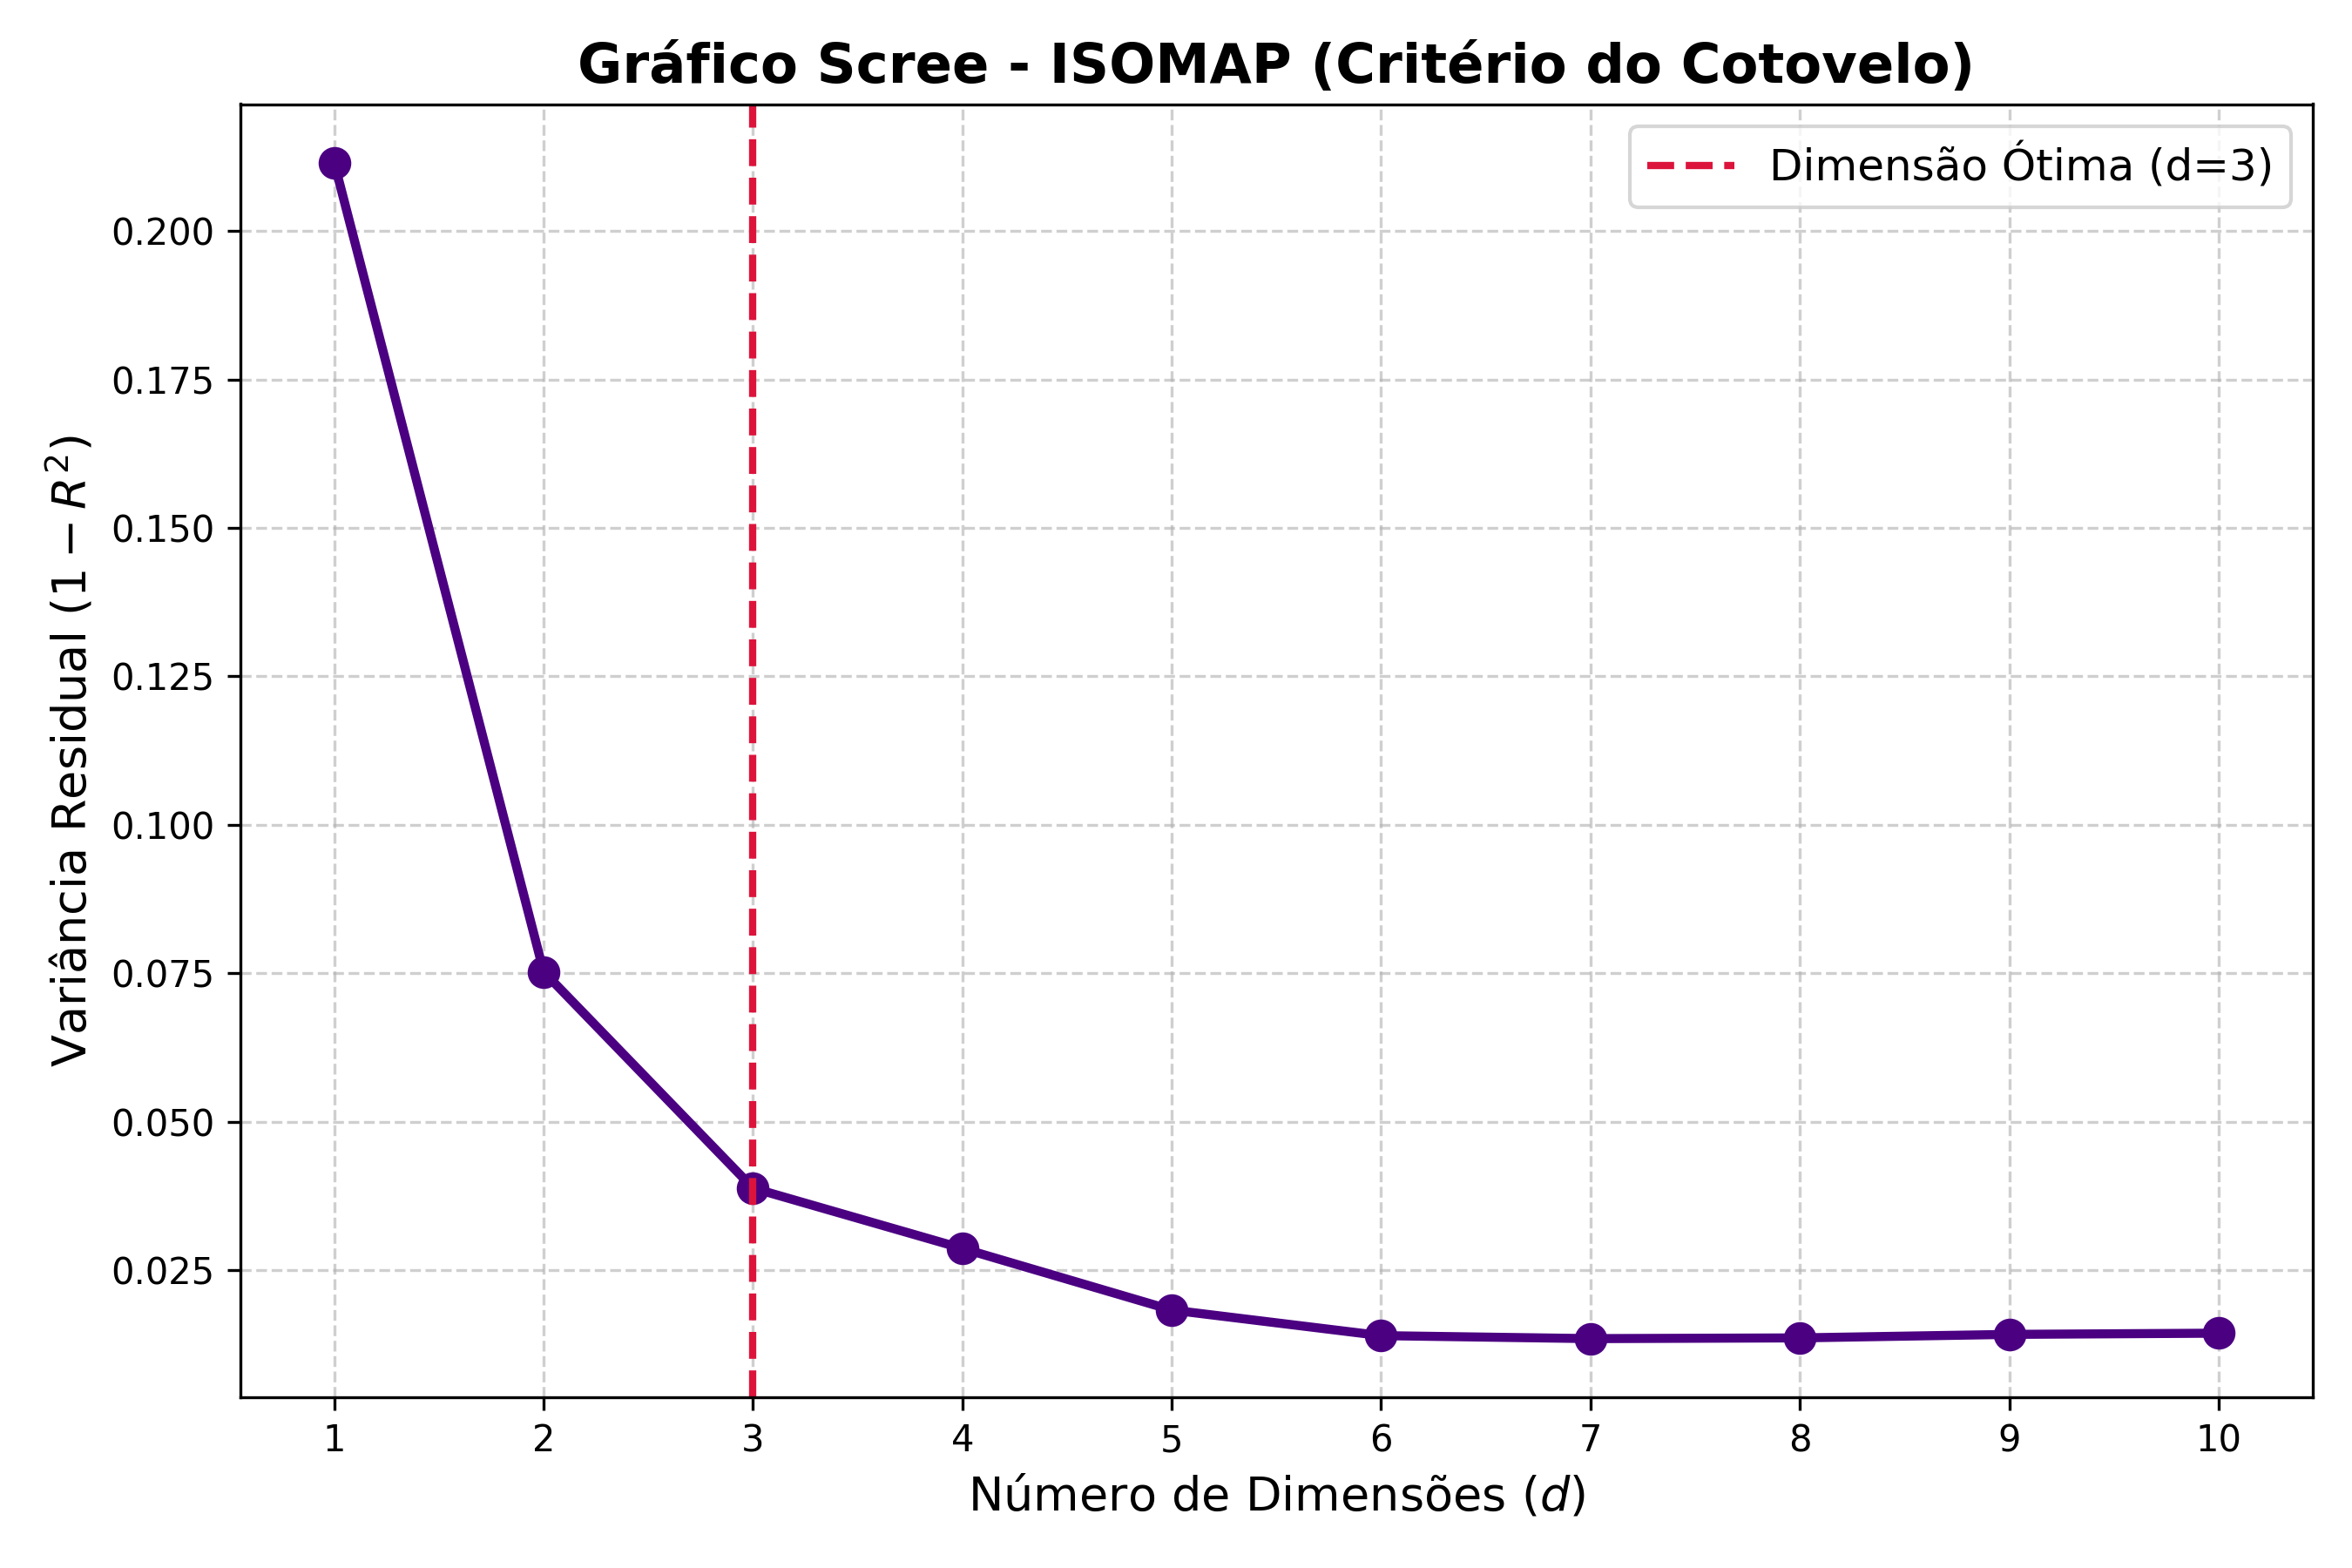
\includegraphics[width=0.6\textwidth]{Imagens/grafico_scree_isomap.png}
    
    \caption{ Redução de dimensão via Isomap para a estrutura 1OMP. A flexão abrupta no parâmetro $d=3$ indica a dimensionalidade intrínseca ideal para a representação das flutuações dinâmicas da MBP.}
    \label{fig:grafico_scree} 
\end{figure}

\subsection{Classificação com SVM}\label{secao_svm}

\ident Com o espaço de dados modelado e visualmente compreensível, o problema de distinguir proteínas abertas de fechadas reduz-se a um problema clássico de reconhecimento de padrões supervisionado. Para essa tarefa, empregamos as Máquinas de Vetores de Suporte (SVM — \textit{Support Vector Machines}), fundamentadas na Teoria do Aprendizado Estatístico de Vapnik e Lorena\cite{Cortes1995, lorena2007}.

\subsubsection{SVM Linear com Margem Rígida}

\ident A SVM linear com margens rígidas definem fronteiras lineares a partir de dados
linearmente separáveis. Seja $T$ um conjunto de treinamento com $n$ dados $x_i \in X$ e seus respectivos rótulos $y_i \in Y$, em que $X$ constitui o espaço dos dados e $Y = \{-1, +1\}$. $T$ é linearmente separável se é possível separar os dados das classes $+1$ e $-1$ por um hiperplano dado pela equação:
\begin{equation}\label{eq: hiperplano}
    f(x) = w \cdot x + b = 0
\end{equation}
em que $w \cdot x$ é o produto escalar entre os vetores $w$ e $x, w \in X$ é o vetor normal ao hiperplano descrito e $\frac{b}{\lVert w\rVert}$ corresponde à distância do hiperplano em relação à origem, com $b \in \mathfrak{R}$.

\ident A equação \eqref{eq: hiperplano} divide o espaço dos dados $X$ em duas regiiões: $w \cdot x + b > 0$ e $w \cdot x + b < 0$.  Podemos definir a função sinal
\begin{equation*}
    g(x) = \sgn (f(x)) = \begin{cases}
        +1 \quad \text{se} \,\, w \cdot x + b > 0 \\
        -1 \quad \text{se} \,\, w \cdot x + b < 0
    \end{cases}
\end{equation*}
que tem como finalidade a obtenção das classificações. 



\ident A partir de $f(x)$, é possível obter um número infinito de hiperplanos equivalentes, pela multiplicação de w e b por uma mesma constante. Define-se o hiperplano canônico em relação ao conjunto $T$ como aquele em que $w$ e $b$ são escalados de forma que os exemplos mais próximos ao hiperplano $w \cdot x + b = 0$ satisfaçam a equação
\begin{equation*}
    \left|w \cdot x_i + b\right| = 1
\end{equation*}
que implica em:
\begin{align*}
    &\begin{cases}
        w \cdot x_i + b \geq +1 \quad \text{se} \,\, y_i = +1 \\
        w \cdot x_i + b \leq -1 \quad \text{se} \,\, y_i = -1
    \end{cases}
    \\\\
    \implies &y_i(w \cdot x_i + b ) \geq 1, \forall(x_i, y_i) \in T.
\end{align*}

\ident Seja $x_1$ um ponto no hiperplano $H_1:w \cdot x + b = +1$ e $x_2 $um ponto no hiperplano $H_2:w \cdot x + b = -1$ projetando $x_1 - x_2$ na direção de $w$,
perpendicular ao hiperplano separador $w \cdot x + b = 0$, é possível obter a distância entre os hiperplanos $H_1$ e $H_2$ dada por
\begin{equation*}
    (x_1 - x_2)\left(\frac{w}{\lVert w \rVert} \cdot \frac{(x_1 - x_2)}{\lVert x_1 - x_2\rVert}\right).
\end{equation*}

\ident Tem-se que $w \cdots x_1 + b = +1$ e $w \cdots x_2 + b = -1$. A diferença entre essas equações fornece $w \cdot (x_1 - x_2) = 2$, logo, obtem-se:
\begin{equation*}
    \frac{2}{\lVert w \rVert} \cdot \frac{(x_1 - x_2)}{\lVert x_1 - x_2\rVert}
\end{equation*}
Como deseja-se obter o comprimento do vetor projetado, toma-se que a distância $d=\frac{2}{\lVert w \rVert}$ entre os hiperplanos $H_1$ e $H_2$, paralelos ao hiperplano separador. Como $w$ e $b$ foram escalados de forma a não haver exemplos entre $H_1$ e $H_2$, $\frac{1}{\lVert w \rVert}$ é a distância mínima entre o hiperplano separador e os dados de treinamento. Essa distância é definida como a margem geométrica do classificador linear.

\begin{figure}[H]
    \centering
    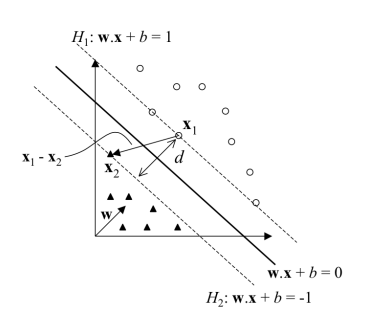
\includegraphics[width=0.5\textwidth]{Imagens/hiperplano_h1_h2.png}
    \caption{Cálculo da distância $d$ entre os hiperplanos $H_1$ e $H_2$. Os dados estão representados por círculos e triângulos. Fonte: retirado de \cite{lorena2007}.}
\end{figure}

\ident Verifica-se que a maximização da margem de separação dos dados em relação a $w \cdot x + b = 0$ pode ser obtida pela minimização de $\lVert w\rVert$. Dessa forma, recorre-se ao seguinte problema de otimização
\begin{align*}
    \min_{w,b} \quad  &\frac{1}{2} \|w\|^2 \\[0.5cm]
    \text{sujeito a} \quad  y_i(w \cdot x_i + b) &\geq 1, \quad \forall i = 1, \cdots, n.
\end{align*}
As restrições são impostas de maneira a assegurar que não haja dados de treinamento
entre as margens de separação das classes. Por esse motivo, a SVM obtida possui também a
nomenclatura de SVM com margens rígidas.

\ident Ao resolver o dual deste problema de programação quadrática através dos multiplicadores de Lagrange $\alpha_i$, que leva-se aos resultados:
\begin{align*}
    \sum_{i=1}^{n}\alpha_i y_i = 0 \quad \text{e} \quad w = \sum_{i=1}^{n}\alpha_i y_i x_i.
\end{align*}
O problema dual obtido da-se por:
\begin{align*}
    \max_{\alpha} \sum_{i=1}^{n}\alpha_i - \frac{1}{2}\sum_{i,j=1}^{n}\alpha_i\alpha_j y_i y_j (x_i \cdot x_j)\\[0.5cm]
    \text{sujeito a} \quad \begin{cases}
        \alpha_i \geq 0, \quad \forall i = 1, \cdots, n\\
        \sum_{i=1}^{n} \alpha_i y_i = 0
    \end{cases}
\end{align*}
É interessante observar também que o problema dual é formulado utilizando apenas os dados de treinamento e os seus rótulos.

\ident Obtida a solução ótima do problema dual, representada pelo vetor de multiplicadores de Lagrange $\alpha^*$, as variáveis primais podem ser restabelecidas. O vetor de pesos $w^*$ é determinado por uma combinação linear ponderada dos dados de treinamento, sofrendo a influência direta apenas das observações cujos multiplicadores associados sejam estritamente positivos ($\alpha_i^* > 0$). Por meio das condições de folga complementar de Karush-Kuhn-Tucker (KKT), esses pontos específicos caracterizam-se geometricamente como os vetores de suporte, posicionados exatamente sobre as margens hiperplânicas. Para todas as demais observações do conjunto de dados, os multiplicadores colapsam para zero ($\alpha_i^* = 0$), tornando-as irrelevantes para a definição geométrica da fronteira de decisão. 

\ident O cálculo do viés ótimo $b^*$ consolida-se a partir do conjunto dos vetores de suporte, denotado por $\mathcal{S}$, computando-se a média aritmética das soluções locais para mitigar instabilidades numéricas, onde $n_{\mathcal{S}}$ representa a cardinalidade de $\mathcal{S}$:
\begin{equation*}
    b^* = \frac{1}{n_{\mathcal{S}}} \sum_{j \in \mathcal{S}} \left( \frac{1}{y_j} - \sum_{i \in \mathcal{S}} \alpha_i^* y_i x_i \cdot x_j \right).
\end{equation*}

\ident Como resultado final deste processo de otimização, estabelece-se a função do classificador linear $g(x)$, a qual projeta novas instâncias e infere seus respectivos rótulos com base na função sinal:
\begin{equation*}
    g(x) = \text{sgn}\left( \sum_{i \in \mathcal{S}} \alpha_i^* y_i x_i\cdot x + b^* \right).
\end{equation*}

Esta função linear representa o hiperplano que separa os dados com maior margem,
considerado aquele com melhor capacidade de generalização.


\subsubsection{SVM Linear com Margem Suave}

\ident Em situações práticas e experimentos empíricos, os dados reais frequentemente apresentam ruídos, \textit{outliers} ou sobreposições espaciais que inviabilizam uma separação puramente linear. Para estender o formalismo clássico a cenários linearmente não-separáveis, introduzem-se as variáveis de folga $\xi_i \geq 0$ para cada instância $i = 1, \dots, n$, as quais relaxam as restrições primais originais:
\begin{equation*}
    y_i \left(w \cdot x + b \right) \geq 1 - \xi_i, \quad \xi_i \geq 0, \quad \forall i = 1, \dots, n
\end{equation*}
\ident Esta modificação suaviza as margens geométricas do classificador, tolerando que determinados elementos se posicionem entre as margens paralelas ou sofram erros de classificação. De modo a regular o compromisso entre a maximização da margem e a minimização dos erros marginais e de treinamento, o problema de otimização primal é reformulado introduzindo-se uma constante de penalização $C > 0$:
\begin{align*}
    \min_{w, b, \xi} \quad & \frac{1}{2} \|w\|^2 + C \sum_{i=1}^{n} \xi_i \\[0.5cm]
    \text{sujeito a} \quad  y_i \left(w \cdot x + b \right) &\geq 1 - \xi_i, \quad \xi_i \geq 0, \quad \forall i = 1, \dots, n \nonumber
\end{align*}
\ident A constante de regularização $C$ dita o peso atribuído à penalização dos erros perante a complexidade geométrica do modelo. Utilizando novamente o formalismo dos multiplicadores de Lagrange e impondo a anulação das derivadas parciais, obtém-se o seguinte problema de otimização dual:
\begin{align*}
    \max_{\alpha} \quad & \sum_{i=1}^{n} \alpha_i - \frac{1}{2} \sum_{i,j=1}^{n} \alpha_i \alpha_j y_i y_j  \left(x_i \cdot x_j\right) \\[0.5cm]
    \text{sujeito a} \quad & \begin{cases}
        0 \leq \alpha_i \leq C, \quad \forall i = 1, \dots, n \nonumber \\
         \sum_{i=1}^{n} \alpha_i y_i = 0 \nonumber
    \end{cases} 
\end{align*}

\ident Nota-se que esta formulação dual preserva a estrutura algébrica do caso de margens rígidas, diferenciando-se unicamente pelo fato de os multiplicadores $\alpha_i$ estarem limitados superiormente pela constante $C$. No ponto ótimo, o vetor de pesos $w^*$ mantém-se inalterado, e as variáveis de folga ótimas passam a ser calculadas por $\xi_i^* = \max \left(0, 1 - y_i \left( w^* \cdot x + b^* \right) \right)$. Adicionalmente, as condições de folga complementar de KKT para o caso de margens suaves assumem a forma:
\begin{align*}
    \alpha_i^* \left( y_i \left( w^* \cdot x + b^* \right) - 1 + \xi_i^* \right) &= 0 \\
    \left( C - \alpha_i^* \right) \xi_i^* &= 0
\end{align*}

\ident Os dados que satisfazem a condição $\alpha_i^* > 0$ continuam sendo denominados vetores de suporte, dividindo-se em duas categorias. Se $0 < \alpha_i^* < C$, o cumprimento estrito das restrições de KKT exige que $\xi_i^* = 0$, posicionando esses dados exatamente sobre as margens, os quais são denominados vetores de suporte livres. Por outro lado, se os multiplicadores atingem o limite superior ($\alpha_i^* = C$), os pontos caracterizam os vetores de suporte limitados, subdivididos em erros de treinamento (quando $\xi_i^* > 1$), elementos corretamente classificados contidos no interior das margens (quando $0 < \xi_i^* \leq 1$), ou pontos marginalizados limítrofes (quando $\xi_i^* = 0$). 

\ident Por fim, o cálculo do viés ótimo $b^*$ preserva a estabilidade computacional ao mensurar a média aritmética sobre o subconjunto de vetores de suporte livres, ou seja, aqueles que satisfazem a condição $0 < \alpha_i^* < C$. A função de classificação resultante preserva a mesma lei de decisão linear estabelecida para o caso rígido, herdando as propriedades de convergência global promovidas pela otimização convexa.

\subsubsection{SVM Não Linear}

\ident Embora as Máquinas de Vetores de Suporte lineares com margens suaves tolerem ruídos e sobreposições locais, problemas complexos do mundo real frequentemente exigem fronteiras de decisão estritamente não-lineares. Para estender o formalismo clássico a cenários linearmente não-separáveis, projeta-se o espaço de entradas original para um novo espaço de dimensão superior, denominado espaço de características. Esta estratégia é fundamentada pelo Teorema de Cover, o qual postula que um conjunto de dados não-linear pode ser transformado, com alta probabilidade, em um espaço onde os padrões sejam linearmente separáveis, desde que a transformação seja não-linear e a dimensionalidade do espaço de características seja suficientemente elevada.
\begin{figure}[H]
    \centering
    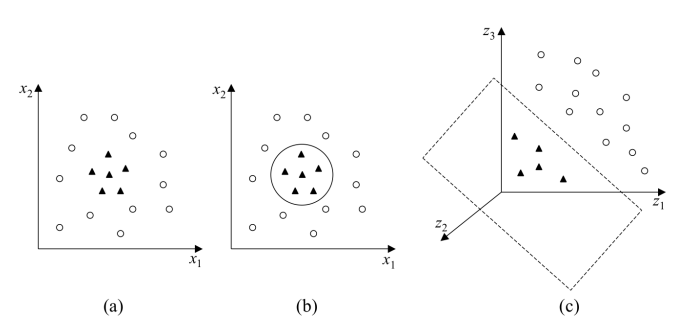
\includegraphics[width=0.8\textwidth]{Imagens/svm_nao_linear.png}
    \caption{ (a) Conjunto de dados não linear expressado em 2 dimensões; (b) Fronteira não linear no espaço de entradas; (c)
Fronteira linear no espaço de características representado em 3 dimenssões. Fonte: retirado de \cite{lorena2007}.}
\end{figure}

\ident Ao aplicar um mapeamento não-linear $\Phi$ ao problema de otimização dual e à função de decisão do classificador, nota-se que as instâncias do conjunto de dados passam a interagir exclusivamente por meio do produto escalar de suas projeções. Sob esta óptica, a função objetivo a ser maximizada assume a forma:
\[
    \max_{\alpha} \quad \sum_{i=1}^{n} \alpha_i - \frac{1}{2} \sum_{i,j=1}^{n} \alpha_i \alpha_j y_i y_j \left( \Phi(x_i) \cdot \Phi(x_j) \right)
\]
\ident Como o espaço de características pode deter dimensionalidade infinita, o cálculo computacional direto de $\Phi$ torna-se inviável. Contudo, a estrutura matemática do problema revela que o conhecimento explícito do mapeamento é desnecessário, exigindo apenas o valor do produto escalar entre os pontos projetados. Esta propriedade viabiliza o uso de funções denominadas \textit{kernels}, as quais computam o produto interno no espaço de características operando unicamente com as coordenadas do espaço original, tal que
\begin{align*}
    K(x_i, x_j) = \Phi(x_i) \cdot \Phi(x_j) .
\end{align*}
Para garantir a convexidade da otimização quadrática e assegurar que a função de \textit{kernel} represente implicitamente um espaço de produto interno válido, exige-se o cumprimento do Teorema de Mercer, o qual dita que as matrizes de \textit{kernel} resultantes sejam simétricas e positivas semidefinidas.

\ident É crucial notar que a aparente necessidade de recorrer a mapeamentos
não-lineares $\Phi$ e a funções de kernel, discutida na formulação geral do
SVM não linear, já se encontra resolvida pela própria construção das
Paisagens de Persistência. Como deduzido na Seção \ref{sec:paisagens_persitencia}, ao adotar o espaço
integrável de Lebesgue com $p=2$, o domínio das paisagens assume
rigorosamente a estrutura de um espaço de Hilbert funcional, munido de um
produto interno $\langle\lambda,\lambda'\rangle_{L^2}$ associado à norma que
define a distância topológica $\Lambda_2$. Por ser um produto interno
genuíno, essa forma bilinear é automaticamente simétrica e semidefinida
positiva, satisfazendo trivialmente as condições exigidas de um kernel de
Mercer -- sem que seja necessário invocar o teorema em sua direção usual
(kernel $\rightarrow$ espaço de Hilbert), já que o espaço de Hilbert e o
mapeamento $\Phi$ (a própria paisagem $\lambda_k(t)$) foram construídos
explicitamente de antemão. Assim, o pré-processamento topológico das
flutuações elásticas desempenha o papel do mapeamento $\Phi$ oculto na
formulação clássica do SVM não linear, transformando a complexidade
combinatória tridimensional da proteína em contornos funcionais já
linearmente separáveis no espaço de Hilbert, o que permite que a lei de
decisão final seja operada de forma estável por um hiperplano linear.:
\[
    g(x) = \text{sgn}\left( \sum_{i \in \mathcal{S}} \alpha_i^* y_i K(x_i, x) + b^* \right).
\]

\subsection{Validação Cruzada}

\ident A validação de um classificador estatístico exige a mensuração rigorosa da sua capacidade de generalização perante observações não utilizadas durante a etapa de ajuste dos parâmetros de decisão. No escopo da Teoria do Aprendizado Estatístico, o objetivo fundamental é estimar o risco real do modelo, minimizando o viés do estimador de erro. Quando o tamanho amostral $n$ de um domínio de estudo é intrinsicamente restrito, a divisão convencional do conjunto de dados em partições estáticas de treinamento e teste penaliza a convergência dos algoritmos de programação quadrática, induzindo o modelo ao sobreajuste ou à alta variância amostral \cite{lorena2007}. Para contornar essa limitação e extrair um estimador de erro estatisticamente estável, adota-se o método de validação cruzada do tipo \textit{Leave-One-Out} (LOOCV).

\ident Dado um conjunto de dados discreto $\mathcal{D} = \{(x_1, y_1), (x_2, y_2), \dots, (x_n, y_n)\}$, o algoritmo executa um processo iterativo determinístico composto por exatamente $n$ ciclos independentes. Em cada iteração $i$, isola-se uma única instância $(x_i, y_i)$ para atuar como o conjunto de teste unitário, enquanto o modelo é treinado sobre o subconjunto complementar denotado pelo hiperplano ajustado sob a restrição $\mathcal{D} \setminus \{(x_i, y_i)\}$. 

\ident Uma vez estabelecida a função de decisão parcial $g^{\setminus i}(x)$ em cada iteração, realiza-se a predição sobre o elemento excluído $x_i$. A estimativa global do erro de generalização do classificador, denominada erro de \textit{Leave-One-Out}, é computada formalmente por meio da média aritmética dos erros locais mensurados pela função indicadora de perda ao longo de todas as $n$ realizações:
\begin{equation}
    \mathcal{E}_{\text{LOO}} = \frac{1}{n} \sum_{i=1}^{n} I\left( g^{\setminus i}(x_i) \neq y_i \right)
\end{equation}
onde $I(\cdot)$ assume o valor unitário se a classificação for incorreta e zero em caso de acerto. O Teorema de Luntz e Brailovsky demonstra que este procedimento fornece um estimador quase não-enviesado do erro de generalização real, conferindo estabilidade matemática e blindagem estatística à modelagem preditiva aplicada sobre espaços funcionais pontuais.

\begin{remark}
Com a fundamentação detalhada de todo o arcabouço biofísico do modelo elástico de redes, o formalismo abstrato da homologia persistente e a regularização matemática das paisagens de persistência em espaços de Hilbert integráveis para a convergência de classificadores convexos, a base teórica encontra-se plenamente consolidada. O capítulo subsequente descreve a execução prática deste encadeamento analítico sobre as conformações tridimensionais, mapeando o protocolo computacional e os critérios de validação empírica adotados.
\end{remark}

\section{O Desvio Quadrático Médio (RMSD)}\label{sec:rmsd}

\ident Na biofísica estrutural, a métrica canônica para quantificar a dissimilaridade
geométrica entre duas conformações de uma mesma macromolécula é o Desvio
Quadrático Médio (RMSD --- \emph{Root-Mean-Square Deviation}). Neste trabalho,
o RMSD atua como métrica de base, fornecendo uma medida puramente estática e
euclidiana da diferença entre as conformações Apo e Holo da MBP, e estabelecendo
o referencial de comparação para as métricas topológicas exploradas nos
resultados.

\ident Como as proteínas podem estar representadas em referenciais arbitrários de
$\mathbb{R}^3$, o cálculo do RMSD não é uma diferença ponto a ponto: é
necessário resolver um problema de otimização, encontrando a isometria
(rotação e translação) que minimiza a distância entre os dois conjuntos de
pontos \cite{maiorov1994}.

\subsection{RMSD de Coordenada e o Problema da Superposição Ótima} \label{secao_alg_kabsch}

\ident Sejam $V,W \in \mathbb{R}^{N\times 3}$ as matrizes de coordenadas dos $N$
carbonos-alfa de duas conformações da MBP. O RMSD de coordenada ótimo é
definido como
\begin{equation*}
    \mathrm{RMSD}(V,W) = \min_{R,\,\vec t}
    \sqrt{\frac{1}{N}\sum_{i=1}^{N}\left\| R v_i + \vec t - w_i \right\|^2},
    \label{eq:rmsd_coord}
\end{equation*}
em que $R$ é uma matriz de rotação própria ($R^TR=I$, $\det R = 1$) e $\vec t$
um vetor de translação. Removendo-se a translação por centralização em torno
dos centros de massa, o problema reduz-se a
\begin{equation}
    D^2(V,W) = R_V^2 + R_W^2 - 2v,
    \label{eq:rmsd_reducido}
\end{equation}
onde $R_V^2,R_W^2$ são os raios de giração e $v\ge 0$ é a correção ótima de
rotação, dada em função dos valores singulares da matriz de correlação
cruzada $C = \frac{1}{N}\sum_i v_i' w_i'^{\,T}$ (Apêndice \ref{apx:rmsd}). A solução exata
e determinística de $R$ é obtida pelo Algoritmo de Kabsch, via
Decomposição em Valores Singulares (SVD) de $C$.

\begin{algorithm}[H]
\caption{Cálculo do RMSD Ótimo (Algoritmo de Kabsch)}
\label{alg:rmsd}
\linespread{1.3}\selectfont
\begin{algorithmic}[1]
\Require Matrizes de coordenadas $V, W \in \mathbb{R}^{N \times 3}$.
\Ensure Valor escalar do RMSD ótimo entre as estruturas.

\Statex \textbf{Passo 1: Centralização}
\State Calcule os centros de massa $\bar{v}$ e $\bar{w}$.
\For{$i = 1$ \textbf{até} $N$}
    \State $v'_i \leftarrow v_i - \bar{v}$
    \State $w'_i \leftarrow w_i - \bar{w}$
\EndFor

\Statex \textbf{Passo 2: Matriz de Covariância e SVD}
\State Construa a matriz de covariância $C = \sum_{i=1}^N (v'_i)(w'_i)^T$.
\State Compute a SVD de $C$: $[U, \Sigma, \tilde{V}] = \text{SVD}(C)$.

\Statex \textbf{Passo 3: Rotação Ótima}
\State $d \leftarrow \text{sgn}(\det(\tilde{V} U^T))$
\State Defina $S = \text{diag}(1, 1, d)$.
\State $R \leftarrow \tilde{V} S U^T$

\Statex \textbf{Passo 4: Cálculo da Distância}
\State $\text{soma} \leftarrow 0$
\For{$i = 1$ \textbf{até} $N$}
    \State $\text{soma} \leftarrow \text{soma} + \|R v'_i - w'_i\|^2$
\EndFor
\State \Return $\sqrt{\text{soma} / N}$
\end{algorithmic}
\end{algorithm}

\subsection{Limitações do RMSD como Padrão de Comparação}

\ident O RMSD, mesmo otimamente calculado, carece de uma escala absoluta de
interpretação: não é evidente a partir de que valor duas conformações devem
ser consideradas ``distintas''. Maiorov e Crippen \cite{maiorov1994}
mostraram, a partir de comparações exaustivas entre pares de proteínas
globulares similares e dissimilares, que existe um \emph{cutoff} intrínseco
$D_0$, o menor RMSD compatível com um rearranjo cooperativo não trivial da
cadeia, e um segundo limiar $D_1$, correspondente ao nível de
similaridade superado por apenas cerca de $1\%$ dos pares de conformações
compactas aleatórias. Ambos escalam com o comprimento da cadeia $N_{\mathrm{res}}$
segundo uma lei do tipo
\begin{equation*}
    D_{\text{cutoff}} = a + b\,(N_{\mathrm{res}})^{1/3}.
\end{equation*}
\ident Essa dependência empírica evidencia que qualquer cutoff fixo de RMSD (como o
tradicional $3\,\text{\AA}$) é arbitrário fora do contexto do comprimento e
da compacidade da cadeia avaliada, e que o RMSD, por ser uma métrica
puramente geométrica e local, não captura correlações dinâmicas globais entre
resíduos distantes na estrutura primária mas próximos na dinâmica, a
motivação central para a adoção da Homologia Persistente no Capítulo \ref{sec:homologia_persistente}. A
dedução completa do Algoritmo de Kabsch e da análise de significância
estatística do RMSD encontra-se detalhada no Apêndice \ref{apx:rmsd}.

\section{Metodologia}

\ident Com a fundamentação teórica e biológica devidamente estabelecida nos capítulos anteriores, este capítulo destina-se a descrever o processo computacional aplicado à Proteína de Ligação à Maltose (MBP). O percurso metodológico detalha desde a mineração e filtragem dos dados estruturais brutos — destacando a expansão inédita da base amostral clássica — até a estruturação dos dados no formato exigido pelas métricas topológicas e algoritmos de classificação.

\subsection{Aquisição e Preparação do Conjunto de Dados}

\ident O conjunto de calibração deste trabalho baseia-se nas 14 estruturas da Proteína de Ligação à Maltose (MBP) utilizadas por Kovacev-Nikolic et al. (2016) \cite{kovacev2016}. Para garantir a robustez estatística e avaliar a generalização do modelo, a base de dados foi expandida com a mineração de 29 novas estruturas de alta resolução no \textit{Protein Data Bank} (PDB) \cite{Bernstein1977}. A rotulação das amostras seguiu os metadados cristalográficos de cada arquivo: conformações \textit{Apo} (abertas, sem ligantes) e \textit{Holo} (fechadas, complexadas com maltose ou derivados). Os códigos em Python desenvolvidos para estas etapas estão disponíveis em: \url{https://github.com/AnthonyMrqs/Analise-Topologica-de-Dados.git}.

\ident O processamento dos arquivos brutos (\texttt{.cif}) demandou rotinas automatizadas de limpeza tridimensional para a remoção de ruídos (moléculas de solvente, íons e cadeias redundantes). Utilizando a biblioteca \texttt{ProDy}, os dados foram filtrados para extrair exclusivamente as coordenadas euclidianas $(x,y,z)$ dos átomos de carbono-alfa ($C_\alpha$) da Cadeia A. Este procedimento gerou matrizes espaciais padronizadas de dimensão $370 \times 3$ para cada proteína, estabelecendo a isometria de vértices necessária para a modelagem da rede elástica subsequente.

\subsection{Extração da Dinâmica Estrutural e Construção do Espaço Métrico}

\ident A extração da dinâmica molecular elástica foi realizada sobre as coordenadas espaciais isoladas de carbonos-alfa ($C_\alpha$) via Modelo de Rede Anisotrópica (ANM) \cite{atilgan2001}, utilizando rotinas automatizadas do pacote \texttt{ProDy}. A matriz Hessiana correspondente a cada conformação da MBP foi construída e submetida à decomposição espectral. O comportamento flutuacional global da macromolécula foi capturado por meio do truncamento nos 20 primeiros modos normais não triviais de baixa frequência, gerando matrizes de correlação cruzada $C$ com dimensões estritas de $370 \times 370$ entradas para cada amostra proteica \cite{kovacev2016}.

\ident Para converter o comportamento dinâmico elástico em um espaço pseudométrico apto para a computação topológica, aplicou-se a transformação projetiva linear $D_{ij} = 1 - |C_{ij}|$ sobre cada elemento das matrizes de correlação. Essa métrica estabelece que resíduos com acoplamento mecânico perfeito ($|C_{ij}| = 1$) assumam distância dinâmica nula ($D_{ij} = 0$), enquanto oscilações ortogonais ou independentes ($|C_{ij}| = 0$) resultam na distância máxima unitária ($D_{ij} = 1$). O fluxo computacional que integra o processamento físico e o armazenamento estruturado dessas matrizes funcionais está formalizado no Algoritmo \ref{alg:anm_pipeline}.

% ==========================================================
% PARTE 1: Vai ficar exatamente aqui no texto
% ==========================================================
\begin{algorithm}[H]
\caption{Fluxo Computacional para Extração da Matriz de Distância Dinâmica}
\label{alg:anm_pipeline}
\begin{algorithmic}[1]
\Require Lista de identificadores $\mathcal{L} = \{id_1, id_2, \dots, id_M\}$, Categoria da proteína $c$ (Apo/Holo).
\Ensure Salvamento das matrizes de distância em formato binário \texttt{.npy}.

\State $\text{Criar diretórios } \texttt{dataset/c} \text{ e } \texttt{matrizes/c}$
\For{cada identificador $id \in \mathcal{L}$}
    \State \textbf{Etapa 1: Obtenção e Filtragem de Dados}
    \State $\text{arquivo\_cif} \leftarrow \text{ObterEstruturaPDB}(id, \text{formato}=\text{cif})$
    \State $\mathcal{E} \leftarrow \text{AnalisarEstrutura}(\text{arquivo\_cif})$
    \If{$C_\alpha \text{ é nulo}$}
        \State \textbf{continue} \Comment{Descarta estruturas defeituosas}
    \EndIf

    \State \textbf{Etapa 2: Modelagem Física ANM}
    \State $H \leftarrow \text{ConstruirMatrizHessiana}(C_\alpha)$
    \State $[\Lambda, V] \leftarrow \text{CalcularModosNormais}(H)$
\EndFor % Fechamento artificial para o LaTeX não quebrar o compilador
\end{algorithmic}
\end{algorithm}

% ==========================================================
% PARTE 2: Vai quebrar para a página seguinte automaticamente
% ==========================================================
\begin{algorithm}[H]
\ContinuedFloat % <-- Garante que mantém o mesmo número (ex: Algoritmo 3)
\caption{Fluxo Computacional para Extração da Matriz de Distância Dinâmica (Continuação)}
\begin{algorithmic}[1]
\makeatletter \setcounter{ALG@line}{11}
\For{cada identificador $id \in \mathcal{L}$} % Reabertura artificial para manter as linhas verticais/indentação
    \State \textbf{Etapa 3: Matriz de Correlação e Transformação Métrica}
    \State $C \leftarrow \text{CalcularCorrelaçãoCruzada}(\Lambda, V)$ \Comment{Gera matriz $N \times N$}
    \State Inicializar matriz de distância dinâmica $D$ de dimensão $N \times N$
    \For{$i = 1$ \textbf{até} $N$}
        \For{$j = 1$ \textbf{até} $N$}
            \State $D_{ij} \leftarrow 1 - |C_{ij}|$
        \EndFor
    \EndFor
    
    \State \textbf{Etapa 4: Armazenamento Computacional}
    \State $\text{caminho} \leftarrow \text{Concatenar}(\texttt{matrizes/c}, id + \texttt{\_matriz.npy})$
    \State $\text{SalvarBinario}(\text{caminho}, D)$
\EndFor
\end{algorithmic}
\end{algorithm}

\ident A transformação das flutuações tridimensionais nas matrizes de distância funcional de dimensão $370 \times 370$ converteu o sistema biofísico em um espaço pseudométrico discreto. Esta representação matricial constitui o dado de entrada exato sobre o qual serão aplicadas as filtrações simpliciais para a extração dos invariantes topológicos.

\subsection{Filtração de Vietoris-Rips e Paisagens de Persistência}

\ident Para extrair os invariantes topológicos das matrizes de distância funcional $D$, computou-se o complexo simplicial de Vietoris-Rips com limiar de conexão máximo estipulado em $t_{\max} = 0.7$. A progressão geométrica desta filtração computacional, que consolida a topologia estrutural da proteína, é ilustrada na Figura \ref{fig:evolucao_rips}. A partir desta etapa, extraíram-se os diagramas de persistência restritos ao primeiro grupo de homologia ($H_1$), quantificando os ciclos estruturais que modelam a dinâmica tridimensional do sítio de ligação \cite{kovacev2016}.

% --- BLOCO RESERVADO PARA AS SUAS 8 IMAGENS ---
\begin{figure}[H]
    \centering
    % Primeira linha (4 imagens)
    \begin{subfigure}[b]{0.24\textwidth}
        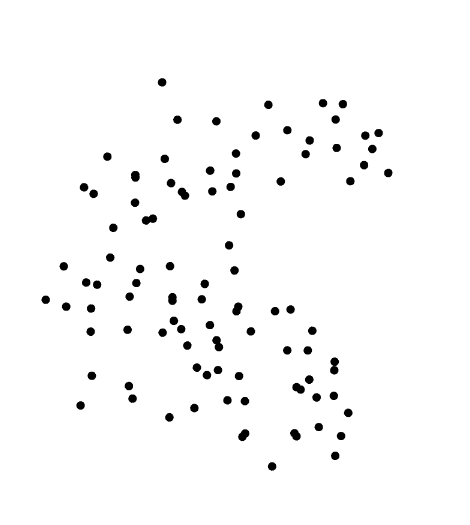
\includegraphics[width=\textwidth]{Imagens/mbp_d1.png}
        \caption{$d = 1.0$Å}
    \end{subfigure}
    \hfill
    \begin{subfigure}[b]{0.24\textwidth}
        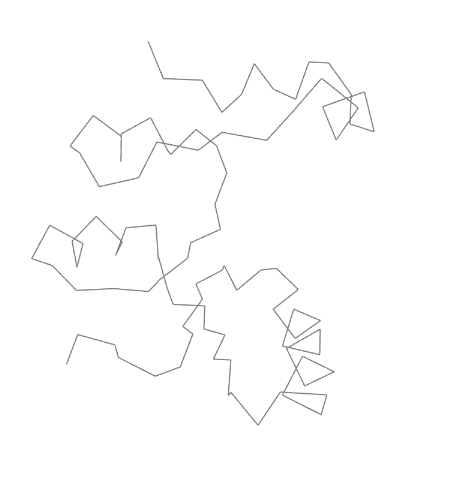
\includegraphics[width=\textwidth]{Imagens/mbp_d4.png}
        \caption{$d = 4.0$Å}
    \end{subfigure}
    \hfill
    \begin{subfigure}[b]{0.24\textwidth}
        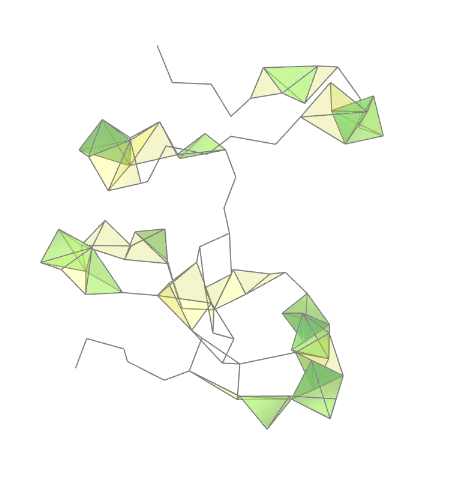
\includegraphics[width=\textwidth]{Imagens/mbp_d55.png}
        \caption{$d = 5.5$Å}
    \end{subfigure}
    \hfill
    \begin{subfigure}[b]{0.24\textwidth}
        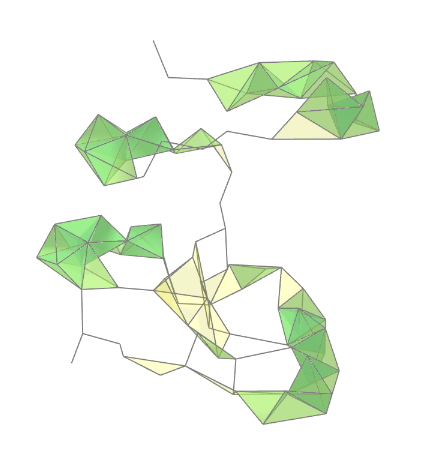
\includegraphics[width=\textwidth]{Imagens/mbp_d6.png}
        \caption{$d = 6.0$Å}
    \end{subfigure}
    
    \vspace{0.5cm} % Espaçamento entre as linhas
    
    % Segunda linha (4 imagens)
    \begin{subfigure}[b]{0.24\textwidth}
        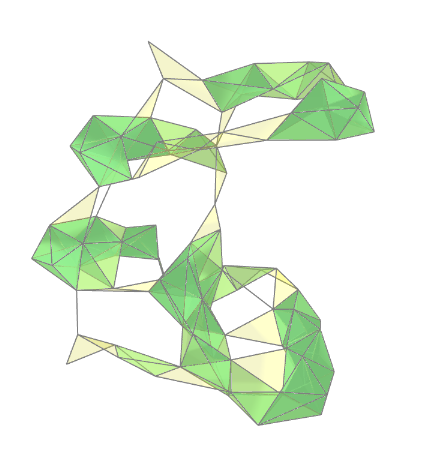
\includegraphics[width=\textwidth]{Imagens/mbp_d7.png}
        \caption{$d = 7.0$Å}
    \end{subfigure}
    \hfill
    \begin{subfigure}[b]{0.24\textwidth}
        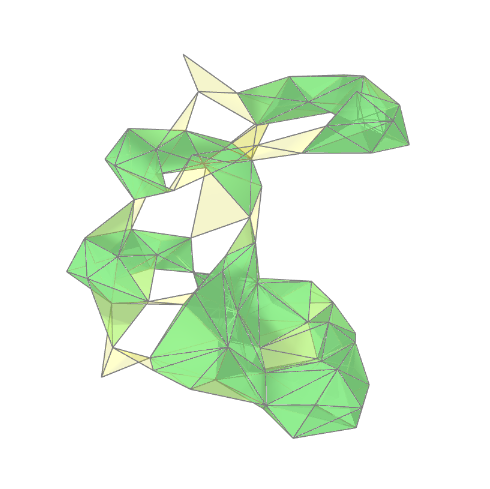
\includegraphics[width=\textwidth]{Imagens/mbp_d8.png}
        \caption{$d = 8.0$Å}
    \end{subfigure}
    \hfill
    \begin{subfigure}[b]{0.24\textwidth}
        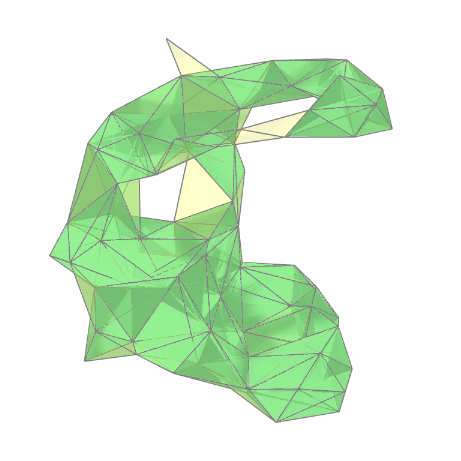
\includegraphics[width=\textwidth]{Imagens/mbp_d9.png}
        \caption{$d = 9.0$Å}
    \end{subfigure}
    \hfill
    \begin{subfigure}[b]{0.24\textwidth}
        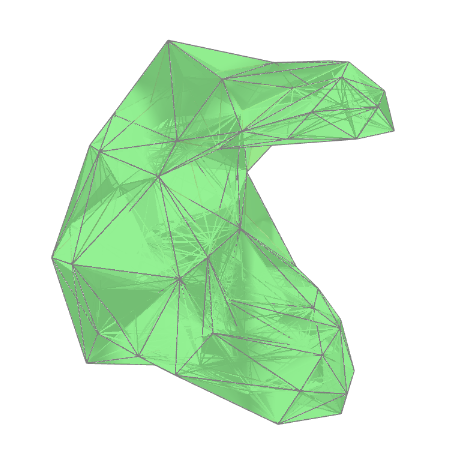
\includegraphics[width=\textwidth]{Imagens/mbp_d12.png}
        \caption{$d = 12.0$Å}
    \end{subfigure}
    \caption{Evolução geométrica do complexo de Vietoris-Rips ao longo da filtração, aplicada sobre uma amostra representativa de 100 carbonos-alfa da estrutura proteica 1OMP. Observa-se a formação progressiva de símplexos de dimensões superiores até a consolidação da topologia global da proteína. As faces de 3-Simplexos são mostradas em verde, os 2-Simplexos em amarelo, os 1-Simplexos como linhas e os 0-Simplexos como pontos.}
    \label{fig:evolucao_rips}
\end{figure}
% ----------------------------------------------

\ident Para contornar a não-linearidade métrica inerente aos diagramas de persistência e viabilizar o uso de algoritmos estatísticos, cada diagrama foi transformado em sua respectiva Paisagem de Persistência \cite{Bubenik2015}. A vetorização contínua empregou três parâmetros fixados analiticamente: limiar restrito ao intervalo $t \in [0.0, 0.7]$ (truncando características infinitas no valor máximo do limiar), discretização em $50$ pontos equidistantes e extração empírica de $73$ camadas funcionais. A Figura \ref{fig:comparativo_landscapes} contrasta o perfil topológico contínuo resultante para ambas as classes estruturais.

% --- BLOCO RESERVADO PARA AS IMAGENS DAS LANDSCAPES ---
\begin{figure}[H]
    \centering
    \begin{subfigure}[b]{0.48\textwidth}
        \centering
        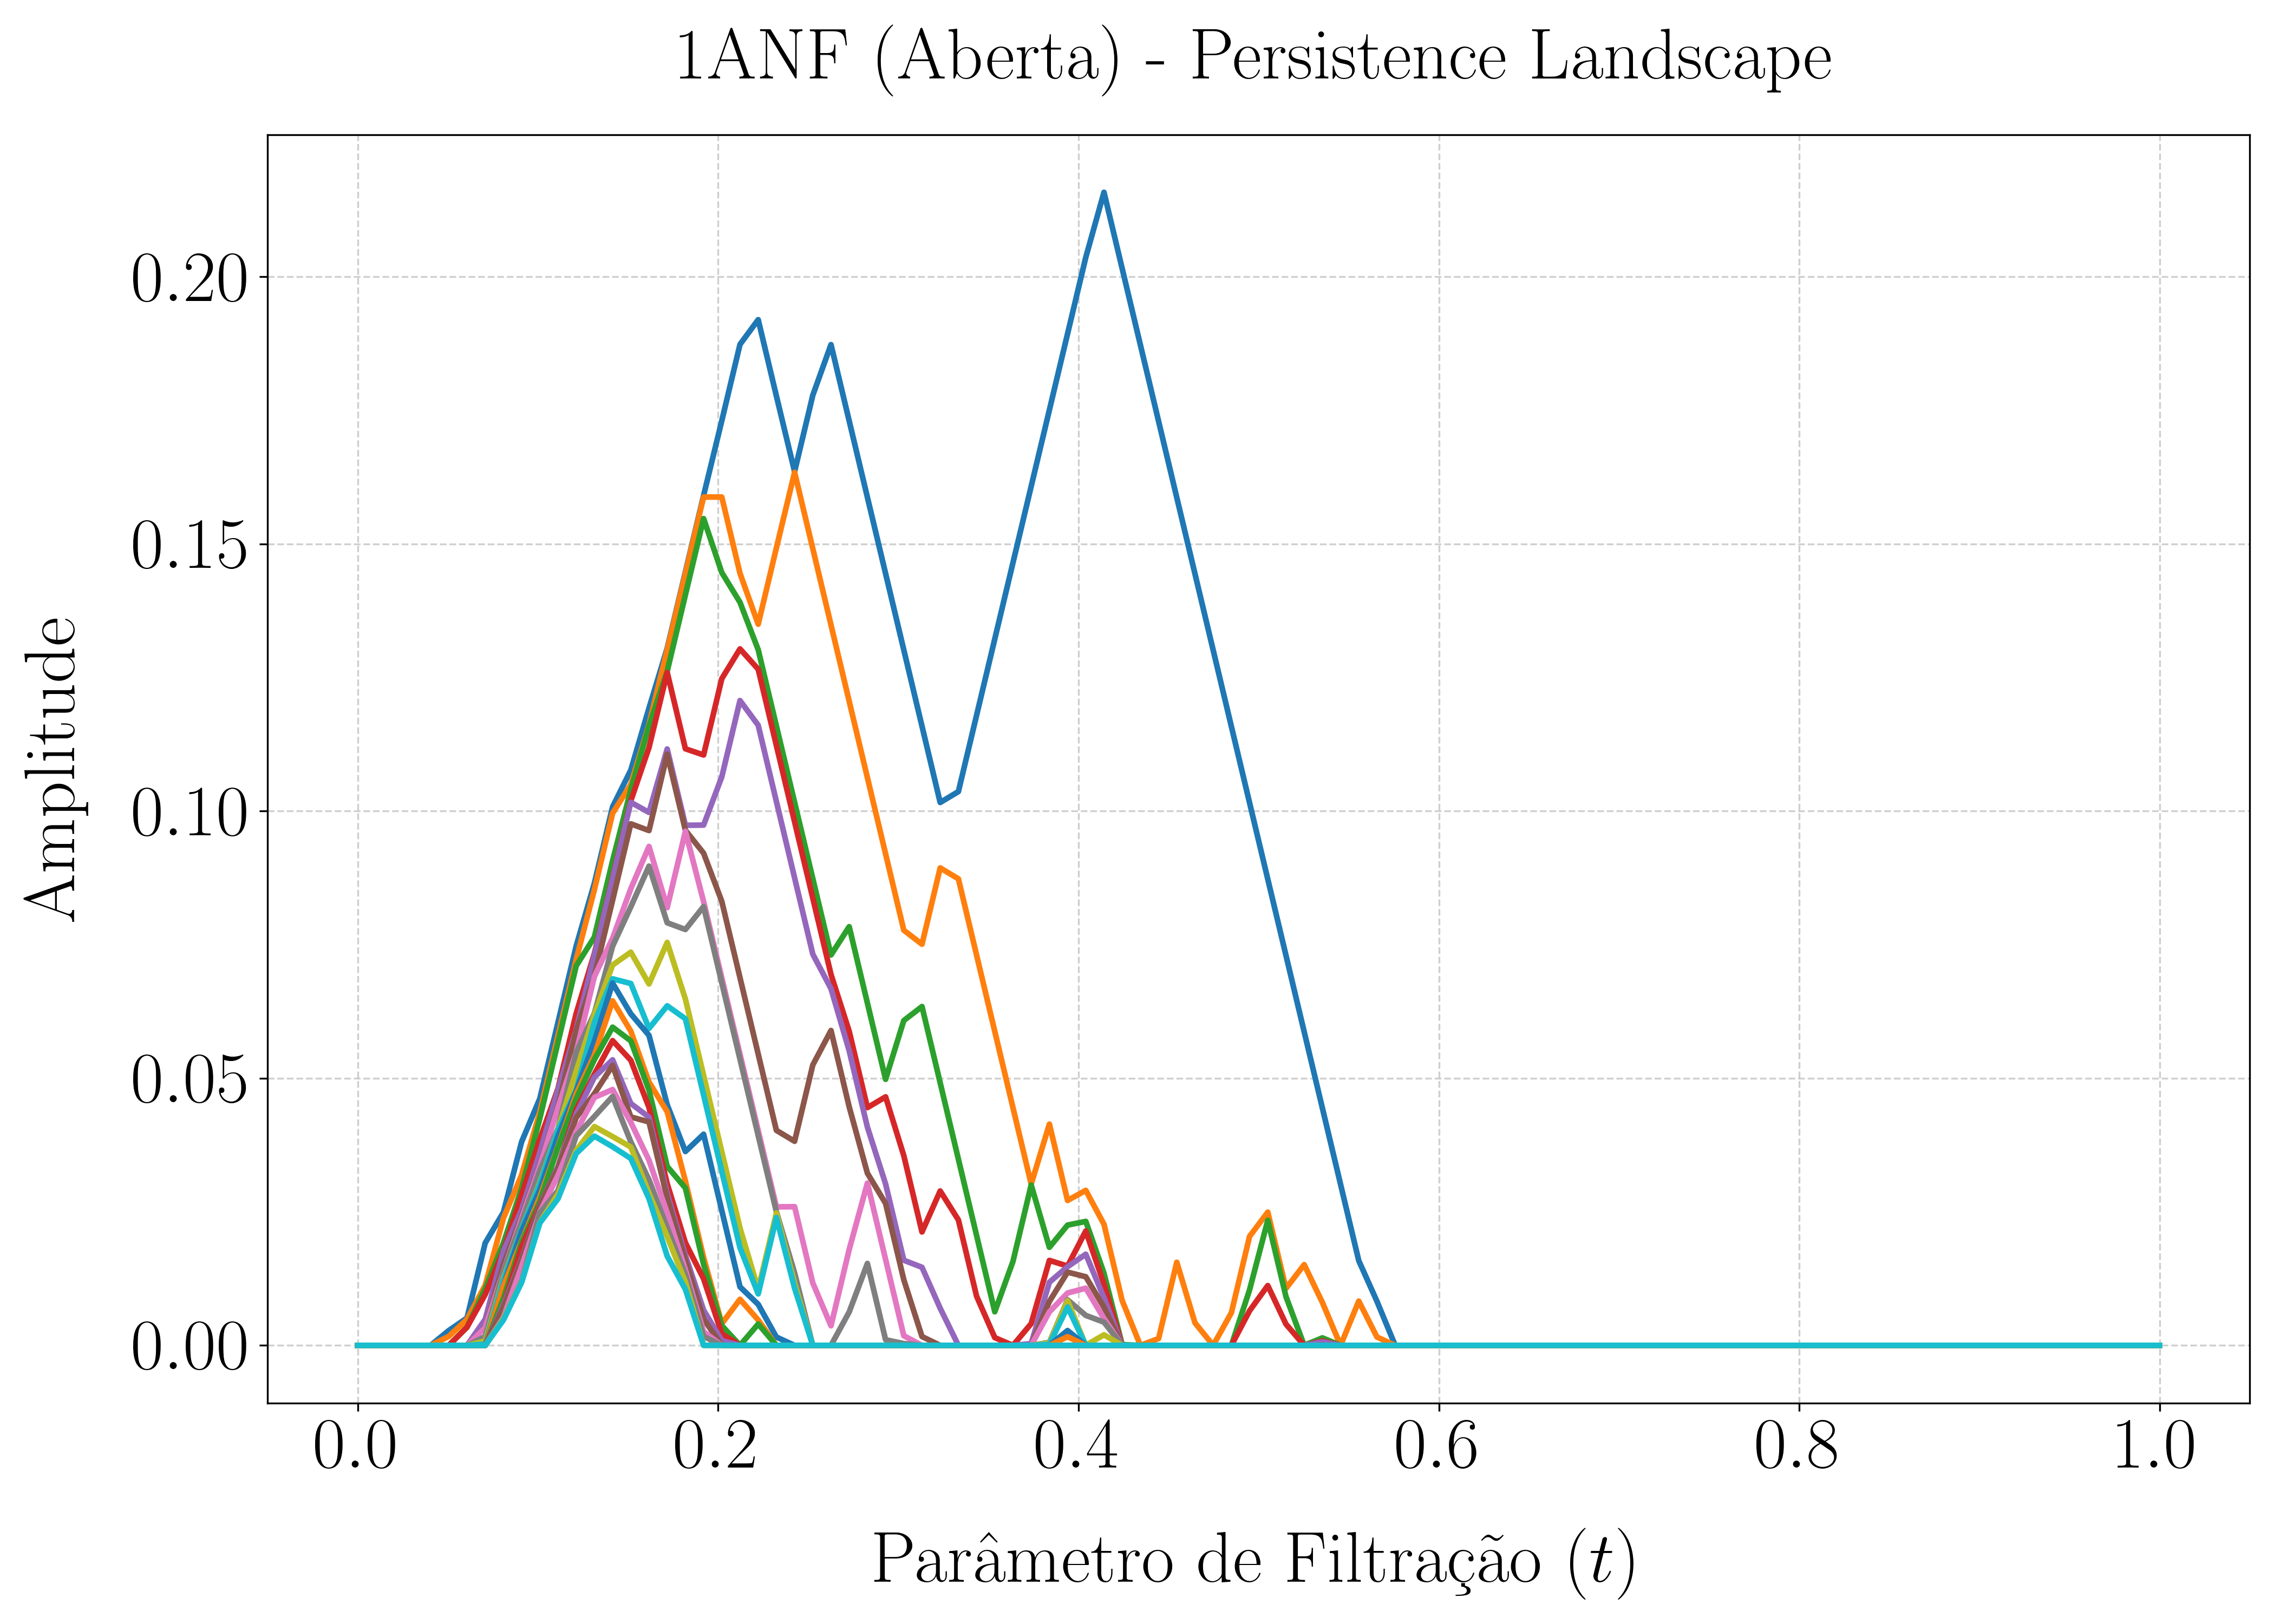
\includegraphics[width=\textwidth]{Imagens/landscape_1ANF.png} % Descomente e insira o nome correto da imagem
        \caption{Estrutura \texttt{1ANF} com conformidade Apo.}
    \end{subfigure}
    \hfill
    \begin{subfigure}[b]{0.48\textwidth}
        \centering
        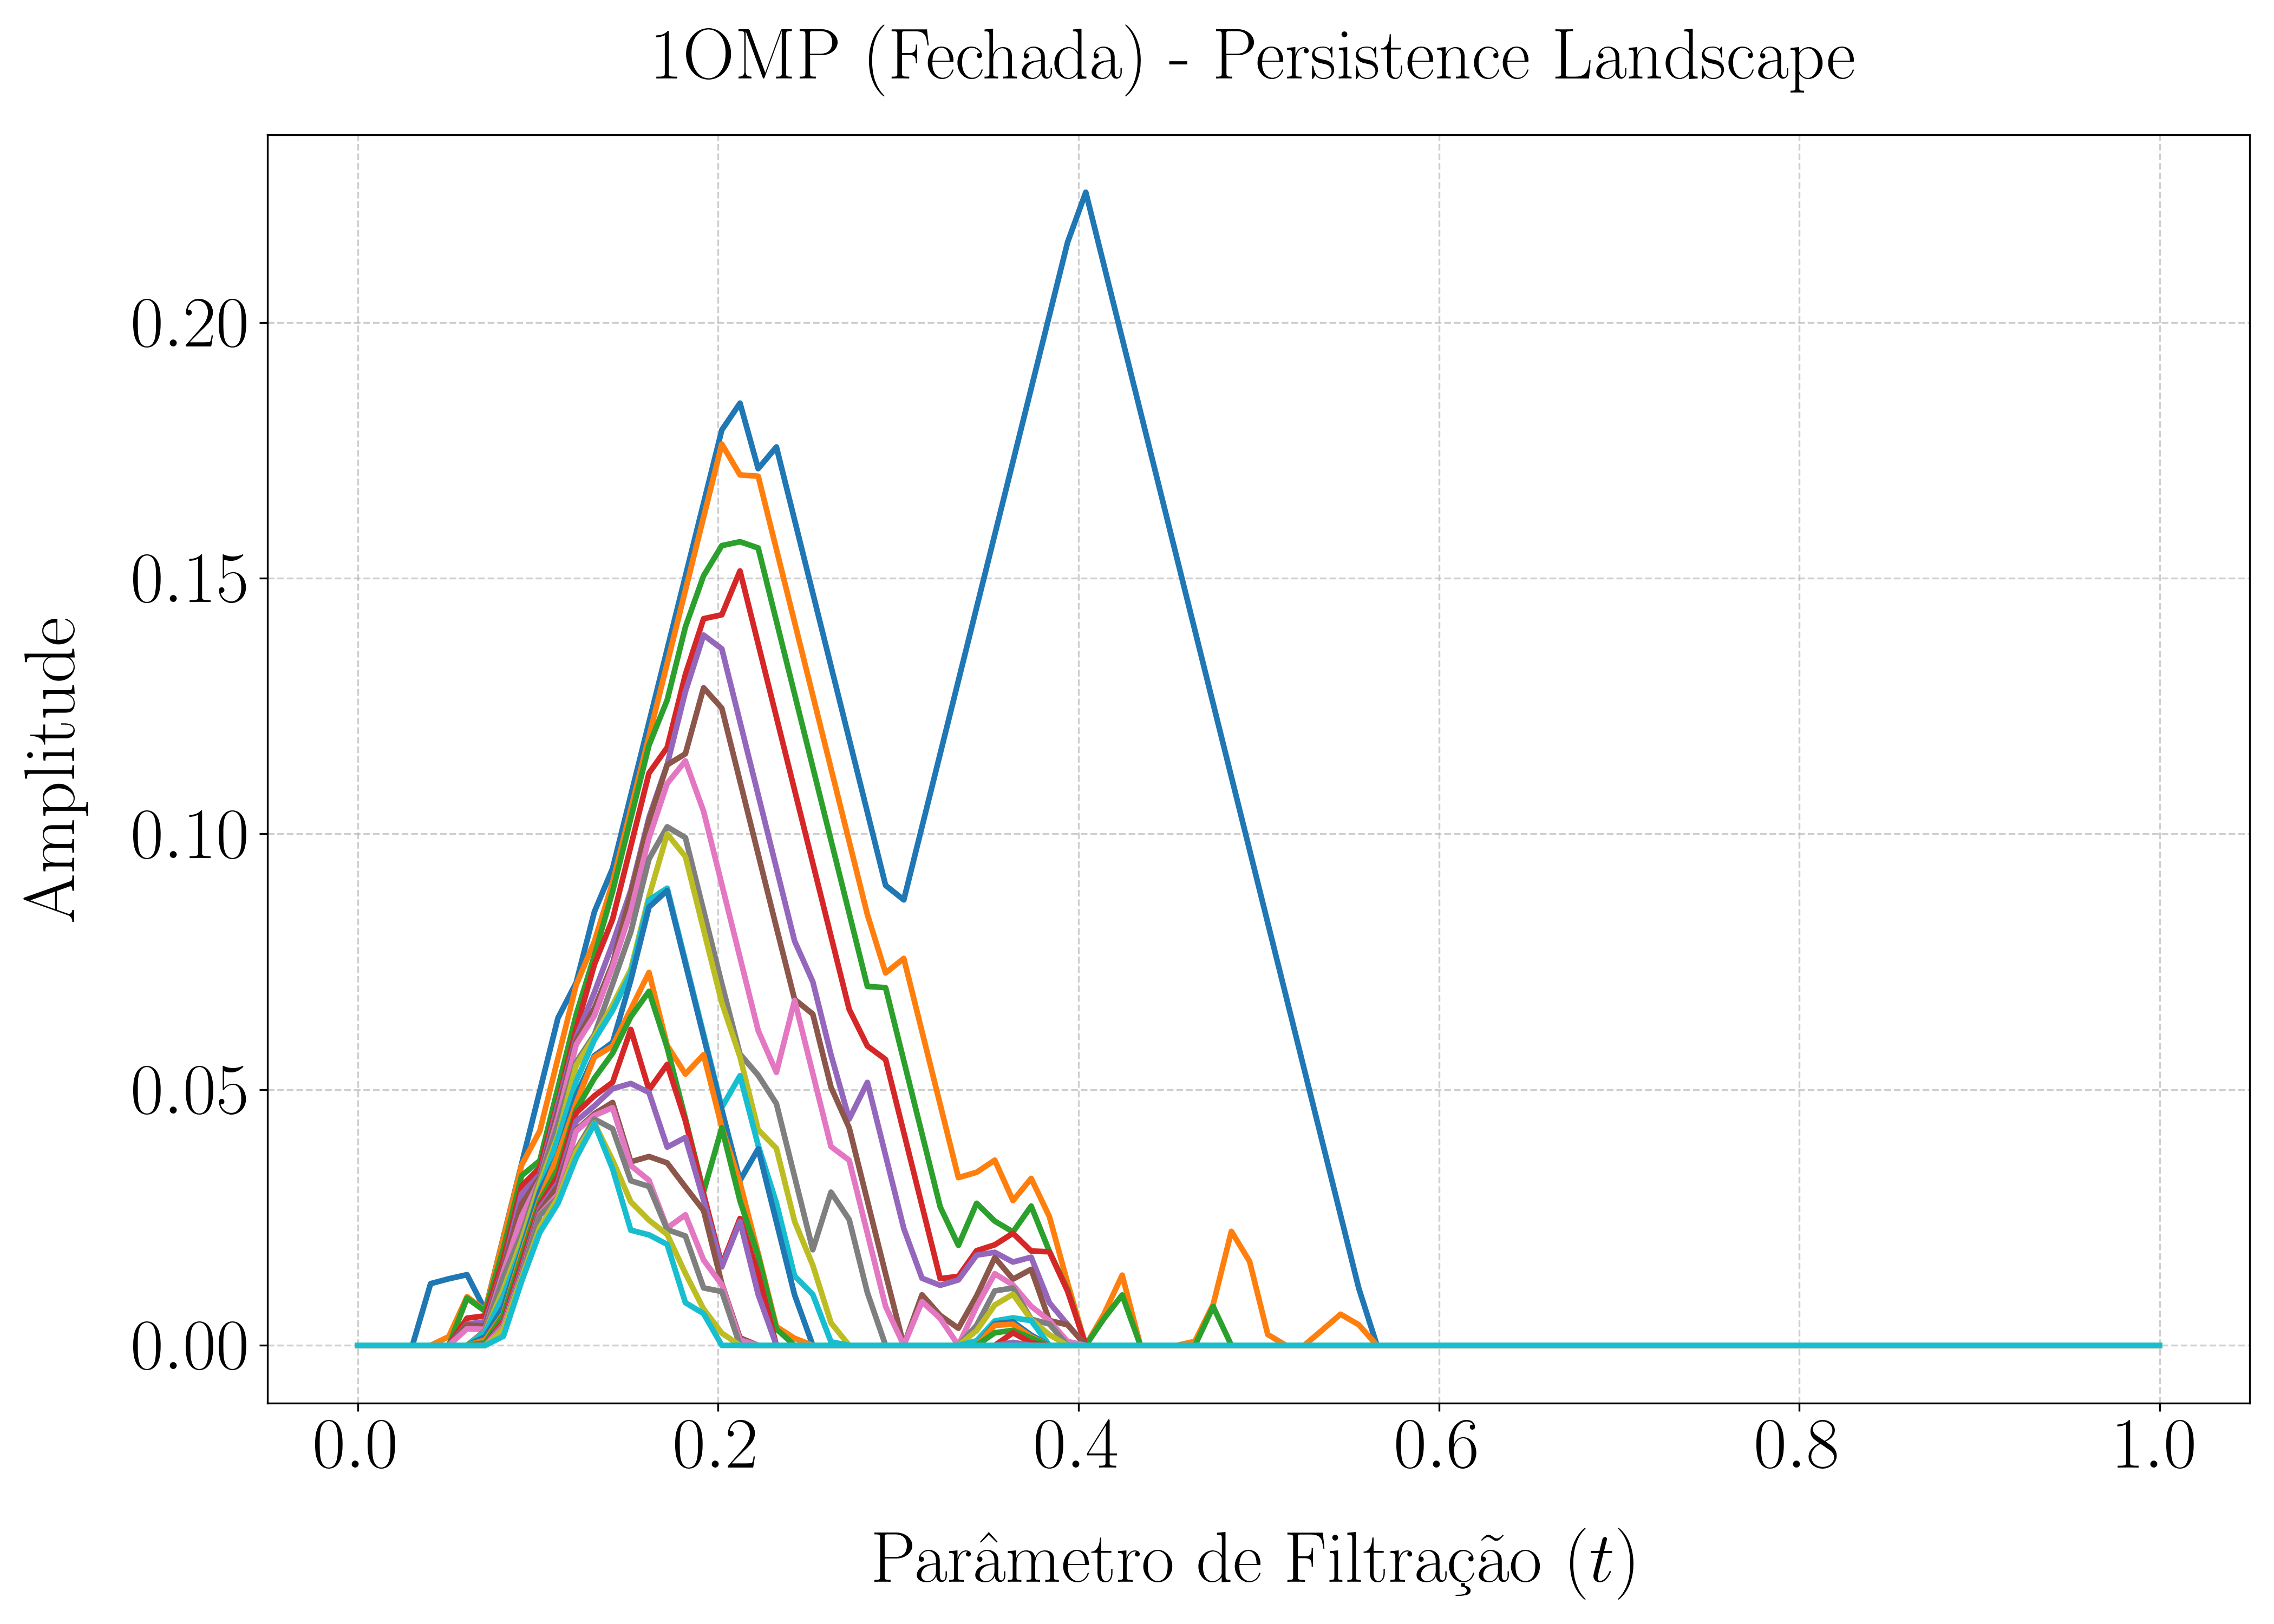
\includegraphics[width=\textwidth]{Imagens/landscape_1OMP.png} % Descomente e insira o nome correto da imagem
        \caption{Estrutura \texttt{1OMP} com conformidade Holo.}
    \end{subfigure}
    \caption{Comparativo visual das Paisagens de Persistência extraídas para o grau homológico $H_1$. A representação mapeia a topologia não-linear das flutuações conformacionais da proteína em um formato funcional vetorial apto para aprendizado de máquina.}
    \label{fig:comparativo_landscapes}
\end{figure}
% ------------------------------------------------------

\ident O fluxo de mapeamento topológico está delineado no Algoritmo \ref{alg:landscapes}. Ao aplanar a matriz funcional, o procedimento extrai um vetor descritor rigoroso de $3650$ dimensões ($73 \times 50$), finalizando a engenharia de dados e posicionando as flutuações da proteína formalmente em um espaço de Banach otimizado para a classificação supervisionada.

\begin{algorithm}[H]
\caption{Computação de Paisagens de Persistência em Espaço de Banach}
\label{alg:landscapes}
\begin{algorithmic}[1]
\Require Matriz de distância $D \in \mathbb{R}^{N \times N}$, grau homológico $g=1$, resolução $R=50$, limiar de escala $t_{\max}=0.7$, número de camadas $K=73$.
\Ensure Vetor descritor unidimensional $v \in \mathbb{R}^{K \times R}$ da paisagem de persistência.

\Statex \textbf{Passo 1: Construção Simplicial e Extração de Homologia}
\State $\mathcal{V} \leftarrow \text{ComplexoVietorisRips}(D, \text{distância máxima} = t_{\max})$
\State $\mathcal{T} \leftarrow \text{CriarArvoreSimplicial}(\mathcal{V}, \text{dimensão máxima} = g+1)$
\State $\mathcal{I} \leftarrow \text{CalcularIntervalosDePersistencia}(\mathcal{T}, \text{grau} = g)$

\Statex \textbf{Passo 2: Tratamento e Truncamento de Singularidades}
\State $\mathcal{I}_{\text{finito}} \leftarrow$ lista vazia
\For{cada intervalo $(\text{nascimento}, \text{morte})$ em $\mathcal{I}$}
    \If{$\text{morte} = \infty$}
        \State $\text{morte} \leftarrow t_{\max}$
    \EndIf
    \State Adicionar $(\text{nascimento}, \text{morte})$ em $\mathcal{I}_{\text{finito}}$
\EndFor

\Statex \textbf{Passo 3: Mapeamento em Paisagem de Persistência}
\If{$\mathcal{I}_{\text{finito}}$ está vazio}
    \State \Return Vetor nulo de dimensão $(K \times R)$
\EndIf
\State $P \leftarrow \text{PaisagemPersistencia}(\text{camadas} = K, \text{resolução} = R, \text{domínio} = [0, t_{\max}])$
\State Matriz funcional $M \leftarrow P.\text{transformar}(\mathcal{I}_{\text{finito}})$

\Statex \textbf{Passo 4: Discretização e Vetorização}
\State \Return $\text{Aplanar}(M)$ \Comment{Achata a matriz funcional em um único vetor}
\end{algorithmic}
\end{algorithm}

\subsection{Redução de Dimensionalidade e Classificação Supervisionada}

\ident Com as flutuações biomoleculares rigorosamente mapeadas num espaço de Hilbert funcional, o problema de distinguir os estados conformacionais resume-se ao reconhecimento de padrões em alta dimensionalidade. O conjunto de vetores extraídos das paisagens de persistência produziu um espaço de características (\textit{features}) composto por 3650 dimensões para cada estrutura proteica. Para viabilizar a convergência de classificadores supervisionados baseados em margem máxima e evitar o fenômeno analítico conhecido como a maldição da dimensionalidade, aplicou-se a Análise de Componentes Principais (PCA), truncando o espaço nas três componentes que capturam a maior variância explicada do sistema tridimensional.

\ident Devido ao tamanho restrito do conjunto de calibração clássico (composto por 14 estruturas devidamente rotuladas), a avaliação da capacidade preditiva do modelo exigiu a aplicação da validação cruzada do tipo \textit{Leave-One-Out} (LOOCV). Do ponto de vista da integridade metodológica, a redução de dimensionalidade e o redimensionamento escalar dos dados (\textit{Standard Scaler}) são processos inerentemente estatísticos que dependem da média e da variância da amostra. Para garantir um estimador de erro estritamente não-enviesado e bloquear qualquer vazamento de informação empírica (\textit{data leakage}) da amostra de teste para o modelo, estabeleceu-se um rigoroso encadeamento de transformações. Em cada iteração da validação cruzada, os hiperparâmetros de padronização e a matriz de projeção do PCA foram ajustados exclusivamente sobre os $N-1$ vetores de treinamento, sendo posteriormente aplicados como uma transformação fixa sobre a única amostra isolada para teste.

\ident O núcleo do aprendizado supervisionado foi operado por uma Máquina de Vetores de Suporte (SVM) parametrizada com um \textit{kernel} linear e constante de regularização $C=1.0$. Conforme justificado no referencial teórico, a adoção de um classificador linear simples sobre os dados projetados é matematicamente suficiente, uma vez que o produto interno das paisagens de persistência em $L^2$ atua nativamente como uma projeção não-linear do domínio físico original. 

\ident A sequência lógica que define a arquitetura de validação iterativa e a construção do classificador global encontra-se consolidada no Algoritmo \ref{alg:ml_pipeline}.

\begin{algorithm}[H]
\caption{Validação LOOCV e Treinamento do Classificador Topológico}
\label{alg:ml_pipeline}
\begin{algorithmic}[1]
\Require Matriz de características $X \in \mathbb{R}^{N \times 3650}$, Vetor de rótulos $Y \in \{-1, +1\}^N$, Conjunto de novas amostras não rotuladas $X_{\text{novas}}$.
\Ensure Acurácia validada do modelo e predição empírica das novas estruturas proteicas.

\Statex \textbf{Passo 1: Validação Cruzada Estrita (Evitando Vazamento de Dados)}
\State $\text{Acertos} \leftarrow 0$
\For{$i = 1$ \textbf{até} $N$}
    \State Particionar dados: $X_{\text{treino}} \leftarrow X \setminus \{X_i\}$, \quad $X_{\text{teste}} \leftarrow \{X_i\}$
    \State Particionar rótulos: $Y_{\text{treino}} \leftarrow Y \setminus \{Y_i\}$, \quad $Y_{\text{teste}} \leftarrow \{Y_i\}$
    
    \State $\mu, \sigma \leftarrow \text{CalcularMediaEVariancia}(X_{\text{treino}})$
    \State $X_{\text{treino}}' \leftarrow \text{Padronizar}(X_{\text{treino}}, \mu, \sigma)$
    \State $X_{\text{teste}}' \leftarrow \text{Padronizar}(X_{\text{teste}}, \mu, \sigma)$ \Comment{Aplica parâmetros do treino}
    
    \State $M_{\text{PCA}} \leftarrow \text{AjustarPCA}(X_{\text{treino}}', \text{componentes} = 3)$
    \State $Z_{\text{treino}} \leftarrow \text{Projetar}(X_{\text{treino}}', M_{\text{PCA}})$
    \State $Z_{\text{teste}} \leftarrow \text{Projetar}(X_{\text{teste}}', M_{\text{PCA}})$ \Comment{Aplica projeção do treino}
    
    \State $\text{Modelo} \leftarrow \text{TreinarSVMLinear}(Z_{\text{treino}}, Y_{\text{treino}}, C=1.0)$
    \If{$\text{Modelo.Prever}(Z_{\text{teste}}) = Y_{\text{teste}}$}
        \State $\text{Acertos} \leftarrow \text{Acertos} + 1$
    \EndIf
\EndFor
\State $\text{Acurácia}_{\text{LOO}} \leftarrow \text{Acertos} / N$

\Statex \textbf{Passo 2: Construção do Modelo Global e Inferência}
\State Ajustar Padronização e PCA sobre a matriz completa $X$.
\State $Z_{\text{global}} \leftarrow \text{Projetar}(X, M_{\text{PCA\_global}})$
\State $\text{Modelo}_{\text{final}} \leftarrow \text{TreinarSVMLinear}(Z_{\text{global}}, Y, C=1.0)$

\State $X_{\text{novas}}' \leftarrow \text{AplicarTransformacoes}(X_{\text{novas}})$
\State $Y_{\text{preditos}} \leftarrow \text{Modelo}_{\text{final}}.\text{Prever}(X_{\text{novas}}')$
\State \Return $\text{Acurácia}_{\text{LOO}}$ e $Y_{\text{preditos}}$
\end{algorithmic}
\end{algorithm}

\ident Concluído este ensaio de validação e obtendo-se o modelo analítico final embasado nos dados de calibração, o escopo metodológico da pesquisa considera-se encerrado. O Ffluxo computacional estabelecido assegura que todas as inferências sobre as novas dezenas de proteínas coletadas apoiem-se sobre métricas invariantes a translações rígidas e validadas estatisticamente. No capítulo subsequente, apresentam-se e discutem-se os resultados numéricos, as visualizações das projeções não-lineares e a eficácia de classificação decorrente desta arquitetura.

\subsection{Modelagem Preditiva e Classificação Geométrica (Baseline)}

\ident Com a vetorização topológica concluída, procedeu-se à etapa de classificação preditiva estrutural. O vetor de características contendo 3650 dimensões (referente ao grau $H_1$) alimentou um classificador do tipo Máquina de Vetores de Suporte (SVM) equipado com um \textit{kernel} linear.

\ident Para avaliar o desempenho do modelo no conjunto de calibração (as 14 estruturas basais), adotou-se a Validação Cruzada \textit{Leave-One-Out} (LOOCV). Dada a alta dimensionalidade dos dados topológicos, a aplicação da Análise de Componentes Principais (PCA) fez-se necessária para reduzir o espaço vetorial às 3 componentes principais de maior variância. Para garantir a lisura matemática do experimento e impossibilitar o vazamento de dados (\textit{data leakage}), estabeleceu-se uma arquitetura sequencial rigorosa: a padronização dos dados (via \textit{StandardScaler}) e a projeção do PCA foram ajustadas (\textit{fit}) \textbf{estritamente} sobre o subconjunto de treinamento de cada iteração da validação cruzada, transformando o dado de teste cego isoladamente a posteriori. A síntese lógica deste modelo classificatório contínuo está detalhada no Algoritmo \ref{alg:svm_topologico}.

\begin{algorithm}[H]
\caption{Classificação Topológica Supervisionada com Proteção contra Vazamento de Dados}
\label{alg:svm_topologico}
\begin{algorithmic}[1]
\Require Matriz de características $X \in \mathbb{R}^{14 \times 3650}$, Vetor de Rótulos $Y \in \{0,1\}^{14}$ (Apo=0, Holo=1).
\Ensure Acurácia validada por LOOCV e treinamento do modelo preditor final.

\Statex \textbf{Etapa 1: Validação Cruzada Estrita (LOOCV)}
\State $\text{Acertos} \leftarrow 0$
\For{$i = 1$ \textbf{até} $14$}
    \State $X_{\text{teste}}, Y_{\text{teste}} \leftarrow X[i], Y[i]$
    \State $X_{\text{treino}}, Y_{\text{treino}} \leftarrow X[-i], Y[-i]$ \Comment{Remove amostra $i$ do treino}
    
    \Statex \indent \textit{Ajuste Sequencial exclusivo no Treinamento}
    \State Padronizador $\leftarrow$ TreinarMédiaEVariância($X_{\text{treino}}$)
    \State $X_{\text{treino\_pad}} \leftarrow$ Padronizador.Transformar($X_{\text{treino}}$)
    
    \State RedutorPCA $\leftarrow$ TreinarPCA($X_{\text{treino\_pad}}$, $\text{componentes}=3$)
    \State $X_{\text{treino\_pca}} \leftarrow$ RedutorPCA.Transformar($X_{\text{treino\_pad}}$)
    
    \State ClassificadorSVM $\leftarrow$ TreinarSVM\_Linear($X_{\text{treino\_pca}}, Y_{\text{treino}}$)
    
    \Statex \indent \textit{Inferência Isulada (Evitando Data Leakage)}
    \State $X_{\text{teste\_pca}} \leftarrow$ RedutorPCA.Transformar(Padronizador.Transformar($X_{\text{teste}}$))
    \State Predição $\leftarrow$ ClassificadorSVM.Prever($X_{\text{teste\_pca}}$)
    
    \If{$\text{Predição} = Y_{\text{teste}}$}
        \State $\text{Acertos} \leftarrow \text{Acertos} + 1$
    \EndIf
\EndFor

\Statex \textbf{Etapa 2: Generalização e Inferência}
\State Repetir treinamento do Padronizador, RedutorPCA e ClassificadorSVM usando o conjunto $X$ completo.
\State Prever classes das 28 novas estruturas proteicas mineradas com o modelo consolidado.
\end{algorithmic}
\end{algorithm}

\ident Como contraponto analítico ao método topológico (\textit{baseline} de validação), foi implementado a classificação puramente geométrica baseada no Desvio Quadrático Médio (RMSD). Empregando o alinhamento de Kabsch sobre os carbonos-alfa idênticos, as estruturas não rotuladas $S$ foram projetadas contra os dois conjuntos de calibração: $\mathcal{A}$ (7 estruturas Apo) e $\mathcal{H}$ (7 estruturas Holo). Para garantir robustez e afastar o viés de uma escolha arbitrária de uma única proteína referencial, a classificação geométrica foi bifurcada em duas abordagens exaustivas:

\textbf{Abordagem 1: Mínimo RMSD Médio.} Computou-se a média aritmética das distâncias geométricas da proteína alvo $S$ contra todas as 7 representações de cada classe, conforme a formulação geométrica:
\begin{equation*}
    \overline{RMSD}_{Apo} = \frac{1}{7} \sum_{i=1}^{7} RMSD(S, \mathcal{A}_i) \quad \text{e} \quad \overline{RMSD}_{Holo} = \frac{1}{7} \sum_{i=1}^{7} RMSD(S, \mathcal{H}_i)
\end{equation*}
A proteína $S$ recebe a rotulação final correspondente ao grupo que minimizar a média calculada ($\arg\min$).

\textbf{Abordagem 2: Análise de Sensibilidade Combinatória.} Para dirimir as incertezas da média, efetuou-se o confronto do alvo $S$ contra todas as combinações cruzadas possíveis dos conjuntos basais ($7 \times 7 = 49$ pares únicos de calibração). A proteína $S$ foi classificada através de uma regra de votação majoritária (conforme Algoritmo \ref{alg:rmsd_sensibilidade}), atribuindo a classe que vencesse a maioria dos 49 combates espaciais diretos.

\begin{algorithm}[H]
\caption{Classificação Geométrica (Abordagem de Sensibilidade Combinatória)}
\label{alg:rmsd_sensibilidade}
\begin{algorithmic}[1]
\Require Estrutura alvo $S$, Conjunto $\mathcal{A}$ com 7 Apo, Conjunto $\mathcal{H}$ com 7 Holo.
\Ensure Rótulo majoritário (Apo ou Holo) e nível de certeza percentual.

\State $\text{VotosHolo} \leftarrow 0$
\State $\text{TotalCombinações} \leftarrow 49$

\For{cada referência $a \in \mathcal{A}$}
    \For{cada referência $h \in \mathcal{H}$}
        \State $\text{DistânciaApo} \leftarrow \text{CalcularRMSD}(S, a)$
        \State $\text{DistânciaHolo} \leftarrow \text{CalcularRMSD}(S, h)$
        
        \If{$\text{DistânciaHolo} < \text{DistânciaApo}$}
            \State $\text{VotosHolo} \leftarrow \text{VotosHolo} + 1$
        \EndIf
    \EndFor
\EndFor

\State $\text{Certeza} \leftarrow (\text{VotosHolo} / \text{TotalCombinações}) \times 100$

\If{$\text{VotosHolo} > (\text{TotalCombinações} / 2)$}
    \State \Return "Holo", $\text{Certeza}$
\Else
    \State \Return "Apo", $(100 - \text{Certeza})$
\EndIf
\end{algorithmic}
\end{algorithm}

\section{Resultados e Discussões}

\ident Com a arquitetura metodológica estabelecida, os modelos geométrico (RMSD) e topológico (SVM) foram aplicados às 29 estruturas proteicas mineradas para validação cruzada independente. O objetivo primário desta etapa foi confrontar o poder de generalização do invariante topológico contínuo ($H_1$) contra a métrica espacial discreta clássica.
\begin{figure}[H]
    \centering
    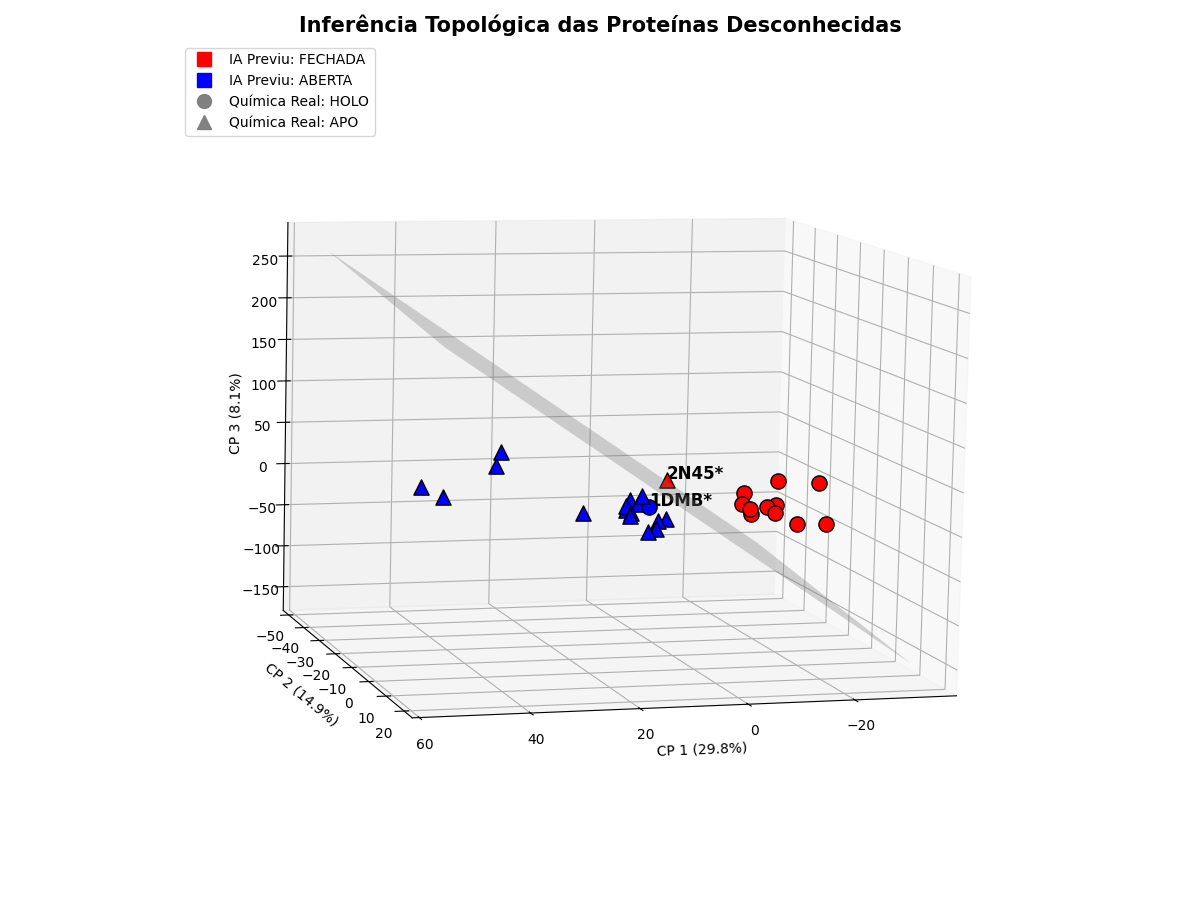
\includegraphics[width=1\textwidth]{Imagens/svm_proteinas.png}
    \caption{Projeção do Hiperplano separando as estruturas por sua classificação.}
\end{figure}
\ident A Tabela \ref{tab:comparativo_geral} consolida os resultados quantitativos da classificação de cada amostra alvo, apresentando as distâncias médias aos conjuntos de calibração ($\overline{RMSD}$), a classe predita pelo critério de distância mínima euclidiana e a respectiva predição do classificador topológico supervisionado (SVM).

\begin{table}[H]
\centering
\resizebox{\textwidth}{!}{%
\begin{tabular}{lcccccc}
\toprule
\textbf{PDB ID} & \textbf{Classe Real} & $\mathbf{\overline{RMSD}_{Fechada}}$ & $\mathbf{\overline{RMSD}_{Aberta}}$ & \textbf{Predição RMSD} & \textbf{Predição SVM} & \textbf{Concordância} \\ 
\midrule
1DMB & Holo & 3.6311 $\pm$ 0.647 & 0.5499 $\pm$ 0.056 & Aberta & Aberta & Concordam (Anomalia)\\
3PUZ & Holo & 1.0227 $\pm$ 1.147 & 3.7854 $\pm$ 0.249 & Fechada & Fechada & Concordam \\
3PV0 & Holo & 1.0463 $\pm$ 1.142 & 3.8214 $\pm$ 0.249 & Fechada & Fechada & Concordam \\
3SER & Holo & 1.2005 $\pm$ 1.061 & 4.1547 $\pm$ 0.247 & Fechada & Fechada & Concordam \\
3SES & Holo & 1.1058 $\pm$ 1.102 & 4.0011 $\pm$ 0.251 & Fechada & Fechada & Concordam \\
3SET & Holo & 1.1346 $\pm$ 1.089 & 4.0753 $\pm$ 0.249 & Fechada & Fechada & Concordam \\
3SEV & Holo & 1.0737 $\pm$ 1.119 & 3.8817 $\pm$ 0.244 & Fechada & Fechada & Concordam \\
3SEW & Holo & 4.1331 $\pm$ 0.715 & 5.4773 $\pm$ 0.171 & Fechada & Fechada & Concordam \\
3SEX & Holo & 1.1368 $\pm$ 1.086 & 3.8916 $\pm$ 0.247 & Fechada & Fechada & Concordam \\
4KHZ & Holo & 0.9955 $\pm$ 1.156 & 3.6966 $\pm$ 0.248 & Fechada & Fechada & Concordam \\
5E24 & Holo & 1.0381 $\pm$ 1.131 & 3.8377 $\pm$ 0.248 & Fechada & Fechada & Concordam \\
8YBE & Holo & 1.2784 $\pm$ 1.042 & 3.9285 $\pm$ 0.250 & Fechada & Fechada & Concordam \\
\midrule
1EZO & Apo & 5.5383 $\pm$ 0.301 & 4.9037 $\pm$ 0.034 & Aberta & Aberta & Concordam \\
1EZP & Apo & 4.6156 $\pm$ 0.428 & 3.4781 $\pm$ 0.038 & Aberta & Aberta & Concordam \\
1MPB & Apo & 3.6619 $\pm$ 0.638 & 0.5185 $\pm$ 0.069 & Aberta & Aberta & Concordam \\
1MPC & Apo & 3.7526 $\pm$ 0.629 & 0.5118 $\pm$ 0.083 & Aberta & Aberta & Concordam \\
1ZIU & Apo & 3.5222 $\pm$ 0.647 & 0.6150 $\pm$ 0.137 & Aberta & Aberta & Concordam \\
1ZJL & Apo & 3.8183 $\pm$ 0.620 & 0.5333 $\pm$ 0.101 & Aberta & Aberta & Concordam \\
1ZKB & Apo & 4.2282 $\pm$ 0.588 & 0.6110 $\pm$ 0.227 & Aberta & Aberta & Concordam \\
1ZMG & Apo & 3.4857 $\pm$ 0.655 & 0.8133 $\pm$ 0.101 & Aberta & Aberta & Concordam \\
2D21 & Apo & 8.6447 $\pm$ 0.365 & 7.6747 $\pm$ 0.054 & Aberta & Aberta & Concordam \\
2H25 & Apo & 2.9788 $\pm$ 0.678 & 2.3371 $\pm$ 0.207 & Aberta & Aberta & Concordam \\
2KLF & Apo & 4.7590 $\pm$ 0.447 & 3.0749 $\pm$ 0.011 & Aberta & Aberta & Concordam \\
2MV0 & Apo & 4.1187 $\pm$ 0.612 & 4.2091 $\pm$ 0.112 & Fechada & Aberta & Divergem \\
2N44 & Apo & 4.4807 $\pm$ 0.425 & 3.6589 $\pm$ 0.087 & Aberta & Aberta & Concordam \\
2N45 & Apo & 3.6403 $\pm$ 0.580 & 2.3491 $\pm$ 0.084 & Aberta & Fechada & Divergem \\
3KJT & Apo & 3.8416 $\pm$ 0.614 & 0.7805 $\pm$ 0.060 & Aberta & Aberta & Concordam \\
7Z7H & Apo & 26.260 $\pm$ 0.040 & 26.799 $\pm$ 0.091 & Fechada & Aberta & Divergem (Artefato)\\
8C8F & Apo & 3.7592 $\pm$ 0.621 & 0.6986 $\pm$ 0.095 & Aberta & Aberta & Concordam \\
\bottomrule
\end{tabular}%
}
\caption{Comparativo de Classificação Estrutural: RMSD Médio vs. Predição Topológica (SVM). Os valores de RMSD estão em Ångströms (Å).}
\label{tab:comparativo_geral}
\end{table}

\ident A análise global da Tabela \ref{tab:comparativo_geral} revela uma robusta consistência entre os métodos geométrico e topológico para a vasta maioria do conjunto de dados, atestando a validade da abstração por Paisagens de Persistência. Contudo, a identificação empírica de falhas no alinhamento métrico e de fronteiras de decisão topológicas forneceu achados matemáticos e biofísicos cruciais, delineados a seguir.

\subsection{Robustez Topológica contra Artefatos de Alinhamento}

\ident O cálculo de métricas espaciais estritas como o RMSD pressupõe correspondência isomórfica perfeita entre os índices atômicos das proteínas. A estrutura \texttt{7Z7H} produziu um erro catastrófico na avaliação de distância euclidiana, com valores de RMSD superando a marca de $26.0$ Å. A inspeção cristalográfica revelou tratar-se de um artefato de modelagem \textit{(mismatch)}: a cadeia iniciava-se no resíduo 5 e apresentava quebras internas de numeração \textit{(gaps)}, deslocando o registro vetorial contra as referências de calibração. 

\ident Sob a ótica geométrica, o modelo perdeu a referencialidade e falhou, rotulando a conformação aleatoriamente como \enquote{Fechada}. Em contrapartida, o processamento topológico operou independentemente de registros ou sistemas de coordenadas rígidos. Ao extrair os invariantes $H_1$ puramente das distâncias relativas entre a nuvem de pontos, o SVM contornou o viés do \textit{gap} estrutural, mantendo sua coesão matemática e classificando a \texttt{7Z7H} com sucesso absoluto em seu estado real de \enquote{Aberta}. Este resultado fundamenta empiricamente a superioridade da Análise Topológica de Dados no manuseio de dados biológicos ruidosos.

\subsection{Variância do Conjunto de Calibração e Análise de Sensibilidade}

\ident A averiguação das matrizes de RMSD evidenciou um desvio padrão considerável no grupo de referências \enquote{Fechadas} (marcadamente em torno de $\sim1.0$ Å a $1.15$ Å). O diagnóstico intra-grupo localizou a fonte analítica da dispersão: a proteína \texttt{3HPI}. Enquanto as demais seis proteínas fechadas mantinham um RMSD interno médio em torno de $1.0$ Å, a \texttt{3HPI} operou como \textit{outlier}, distanciando-se $\sim3.8$ Å do próprio grupo. 

\ident Apesar desta assimetria de envoltório induzida por diferentes ligantes cristalográficos, a aplicação da Abordagem 2 (Análise de Sensibilidade via 49 combinações cruzadas) blindou o diagnóstico métrico. As predições mantiveram confiabilidade majoritária superior a $85\%$ em todos os casos convergentes, assegurando que o referencial geométrico adotado para comparação contra o SVM era sólido e imune ao viés arbitário de calibração.

\subsection{Assinaturas Dinâmicas e as Fronteiras de Decisão}

\ident As anomalias de classificação preditiva forneceram suporte estrutural à teoria de Seleção Conformacional. A proteína \texttt{1DMB} (cadastrada como \textit{Holo}) foi unanimemente julgada como \textit{Aberta} por ambos os métodos, insinuando a existência de falhas de empacotamento ou cristalização incompleta do ligante original no banco de dados.

\ident Contudo, a estrutura \texttt{2N45} configurou o caso mais denso do escopo. Pertencente à classe \textit{Apo}, o RMSD obedeceu à lógica estática e a posicionou firmemente no grupo \textit{Aberta}. No entanto, a modelagem via SVM a enquadrou no lado \textit{Fechado} do espaço de Banach, operando de forma perigosamente adjacente ao hiperplano linear (distância perpendicular de apenas $d=0.1985$). 

\ident Essa discordância isolada não representa uma falha algorítmica, mas a detecção de uma fase de transição contínua. Por utilizar distâncias dinâmicas provenientes das flutuações de B-factor, o método topológico rastreia flexibilidade latente. A classificação limítrofe atesta que a macromolécula, mesmo em ausência de ligantes, amostra energeticamente conformações semi-fechadas de alta frequência, demonstrando a sensibilidade superior da homologia persistente na captura de eventos biomecânicos transientes que são invisíveis aos métodos estáticos puramente espaciais.

\section{Trabalhos Futuros}
\ident Como perspectivas para desdobramentos futuros, propõe-se a expansão desta arquitetura computacional para a análise de trajetórias contínuas de Dinâmica Molecular (MD), viabilizando o rastreamento topológico em tempo real do processo de Seleção Conformacional. Adicionalmente, a exploração de invariantes de ordem superior — como o grupo de homologia $H_2$, ideal para a quantificação precisa de cavidades e bolsões internos — e a integração das Paisagens de Persistência com arquiteturas de \textit{Deep Learning} ou \textit{Kernels} Riemannianos configuram caminhos promissores. Tais avanços visam consolidar a Análise Topológica de Dados como uma ferramenta definitiva não apenas para a classificação estrutural robusta a ruídos, mas para o design racional de ligantes e a descoberta de novos fármacos (\textit{Drug Discovery}) em sistemas macromoleculares de alta complexidade.

\newpage

\appendix

\section{O Modelo de Rede Anisotrópica}
\label{apx:anm}

\ident O Modelo de Rede Anisotrópica (ANM) constitui uma abordagem de grão grosso (\textit{coarse-grained}) fundamentada na física estatística para a simulação da dinâmica de macromoléculas. Diferente de simulações determinísticas completas de Dinâmica Molecular, que integram as equações de Newton para todos os átomos e moléculas de solvente ao longo do tempo, o ANM reduz o custo computacional ao abstrair a estrutura tridimensional da proteína como uma rede elástica tridimensional. Nesta formulação, cada resíduo de aminoácido é representado de forma singular pelas coordenadas espaciais de seu átomo de carbono-alfa ($C_\alpha$), de modo que uma proteína composta por $N$ resíduos é descrita por um vetor de posição $R \in \mathbb{R}^{3N}$.

\ident A premissa mecânica do ANM postula que a estrutura cristalográfica observada corresponde ao estado de mínimo global da energia potencial do sistema. As interações físicas entre os resíduos são modeladas por um potencial harmônico uniforme, onde pares de átomos $i$ e $j$ são conectados por molas elásticas ideais, desde que a distância euclidiana inicial $R_{ij}^0$ entre eles seja inferior a um raio de corte (\textit{cutoff}) empírico $r_c$. A energia potencial total da rede, $V$, que governa as flutuações conformacionais em torno do estado de equilíbrio, é definida analiticamente pela soma quadrática das deformações de todas as molas ativas:
\begin{equation*}
    V = \frac{\gamma}{2} \sum_{i=1}^{N-1} \sum_{j=i+1}^{N} \Gamma_{ij} \left( |R_{ij}| - |R_{ij}^0| \right)^2 \label{eq:anm_potential}
\end{equation*}
onde $\gamma$ é a constante de força elástica macroscópica da mola (assumida como uniforme para todas as interações no modelo padrão), $|R_{ij}|$ é a distância instantânea entre os nós durante a flutuação, e $\Gamma_{ij}$ é o elemento da matriz de conectividade de Kirchhoff, assumindo o valor $1$ se $|R_{ij}^0| \leq r_c$ e $0$ caso contrário.

\ident Para quantificar a anisotropia tridimensional dos movimentos, o potencial de rede é expandido em uma série de Taylor ao redor do estado de equilíbrio. A matriz das segundas derivadas espaciais deste potencial em relação às coordenadas cartesianas ($x, y, z$) forma a Matriz Hessiana do sistema, denotada por $H$. A matriz $H$ é um operador simétrico e semidefinido positivo de dimensão $3N \times 3N$, composta por submatrizes (ou super-elementos) $H_{ij}$ de dimensão $3 \times 3$. Para os elementos fora da diagonal principal ($i \neq j$), cada componente direcional da submatriz Hessiana é calculado pela projeção das distâncias interatômicas de equilíbrio:
\begin{gather*}
    H_{ij} = \begin{bmatrix}
    \frac{\partial^2 V}{\partial x_i \partial x_j} & \frac{\partial^2 V}{\partial x_i \partial y_j} & \frac{\partial^2 V}{\partial x_i \partial z_j} \\
    \frac{\partial^2 V}{\partial y_i \partial x_j} & \frac{\partial^2 V}{\partial y_i \partial y_j} & \frac{\partial^2 V}{\partial y_i \partial z_j} \\
    \frac{\partial^2 V}{\partial z_i \partial x_j} & \frac{\partial^2 V}{\partial z_i \partial y_j} & \frac{\partial^2 V}{\partial z_i \partial z_j}
    \end{bmatrix}\\
    H_{ij} = \frac{-\gamma \Gamma_{ij}}{|R_{ij}^0|^2} \begin{bmatrix}
    (x_j - x_i)^2 & (x_j - x_i)(y_j - y_i) & (x_j - x_i)(z_j - z_i) \\
    (y_j - y_i)(x_j - x_i) & (y_j - y_i)^2 & (y_j - y_i)(z_j - z_i) \\
    (z_j - z_i)(x_j - x_i) & (z_j - z_i)(y_j - y_i) & (z_j - z_i)^2
    \end{bmatrix} \label{eq:hessian_off_diag}
\end{gather*}
\ident A conservação do momento linear e angular exige que a soma dos elementos ao longo de qualquer linha ou coluna da matriz Hessiana seja estritamente nula. Por conseguinte, os super-elementos da diagonal principal ($i = j$), que descrevem a autointeração de cada resíduo com as molas à sua volta, são obtidos pelo somatório negativo dos elementos fora da diagonal de sua respectiva linha, tal que:
\begin{equation*}
    H_{ii} = - \sum_{j \neq i}^{N} H_{ij} \label{eq:hessian_diag}
\end{equation*}
\ident A extração das características termodinâmicas do sistema é realizada por meio da decomposição espectral da matriz Hessiana. O problema de autovalor associado é dado por $H V_k = \lambda_k V_k$, onde $\lambda_k$ representa o $k$-ésimo autovalor (correspondente ao quadrado da frequência natural de vibração do modo $k$) e $V_k$ é o autovetor associado (que descreve a direção do movimento coletivo). Devido às propriedades de invariância translacional e rotacional da estrutura como um corpo rígido no espaço tridimensional, os seis primeiros autovalores da matriz $H$ são nulos ($\lambda_1 = \lambda_2 = \dots = \lambda_6 = 0$). Consequentemente, a verdadeira dinâmica de deformação elástica interna da molécula é descrita pelos $3N - 6$ modos normais ortogonais subsequentes não-triviais.

\ident Finalmente, o comportamento coletivo e as correlações estocásticas entre os deslocamentos de quaisquer dois resíduos $i$ e $j$ são determinados computando-se a matriz inversa pseudogeneralizada da Hessiana ($H^{-1}$). Pelo teorema da equipartição de energia na mecânica estatística clássica, a matriz de covariância espacial das flutuações, denotada por $C$, é proporcional a esta pseudoinversa, sendo expressa analiticamente pela combinação linear dos autovetores ponderada inversamente pelas suas frequências:
\begin{equation}
    C_{ij} \propto \langle \Delta R_i \cdot \Delta R_j \rangle = \frac{k_B T}{\gamma} \sum_{k=7}^{3N} \frac{1}{\lambda_k} \left[ V_k V_k^T \right]_{ij} \label{eq:cross_correlation}
\end{equation}
onde $k_B$ é a constante de Boltzmann e $T$ é a temperatura absoluta do sistema. 

\ident No contexto analítico desta pesquisa metodológica, em conformidade com as práticas consolidadas na biologia estrutural, o somatório integral da Equação \ref{eq:cross_correlation} é truncado. Consideram-se exclusivamente as 20 primeiras frequências não-triviais de vibração ($k = 7$ a $26$). Essa aproximação fundamenta-se no princípio de que os autovalores de menor magnitude dominam exponencialmente a fração da equação, governando assim as grandes transições funcionais globais da proteína — como a transição \textit{Apo}-\textit{Holo} da Proteína de Ligação à Maltose —, enquanto filtram com eficiência o ruído térmico aleatório intrínseco aos modos de alta frequência.

\section{Topologia}
\subsection{Topologia Geral}
\begin{definition}
Um espaço topológico é um par $(X, \mathcal{T})$ onde $X$ é um conjunto e $\mathcal{T}$ é uma coleção de subconjuntos de $X$ tal que:
\begin{itemize}
    \item $\emptyset \in \mathcal{T}$ e $X \in \mathcal{T}$,
    \item para toda coleção infinita $\{O_\alpha\}_{\alpha \in A} \subset \mathcal{T}$, temos $\bigcup_{\alpha \in A} O_\alpha \in \mathcal{T}$,
    \item para toda coleção finita $\{O_i\}_{1 \leq i \leq n} \subset \mathcal{T}$, temos $\bigcap_{1 \leq i \leq n} O_i \in \mathcal{T}$.
\end{itemize}
O conjunto $\mathcal{T}$ é chamado de topologia sobre $X$. Os elementos de $\mathcal{T}$ são chamados de conjuntos abertos.
\end{definition}

\begin{definition}
Seja $(X, \mathcal{T})$ um espaço topológico. Para todo aberto $O \in \mathcal{T}$, seu complementar $cO = \{x \in X \mid x \notin O\}$ é chamado de conjunto fechado.
\end{definition}

\begin{definition}
Seja $x \in \mathbb{R}^n$ e $r > 0$. A bola aberta de centro $x$ e raio $r$, denotada $\mathcal{B}(x, r)$, é definida como:
\[
\mathcal{B}(x, r) = \{y \in \mathbb{R}^n \mid \|x - y\| < r\}.
\]
\end{definition}

\begin{definition}
Seja $A \subset \mathbb{R}^n$ um subconjunto e $x \in A$. Dizemos que $A$ é aberto em torno de $x$ se existe $r > 0$ tal que $\mathcal{B}(x,r) \subset A$. Dizemos que $A$ é aberto se, para todo $x \in A$, $A$ é aberto em torno de $x$.

O conjunto de todos esses abertos é denotado $\mathcal{T}_{\mathbb{R}^n}$ e é chamado de topologia euclidiana sobre $\mathbb{R}^n$.
\end{definition}

\begin{definition}
Seja $(X, \mathcal{T})$ um espaço topológico e $Y \subset X$ um subconjunto. A topologia de subconjunto (ou topologia induzida) sobre $Y$ é o conjunto:
\[
\mathcal{T}|_Y = \{O \cap Y \mid O \in \mathcal{T}\}.
\]
\end{definition}

\begin{definition}
Sejam $(X, \mathcal{T})$ e $(Y, \mathcal{U})$ dois espaços topológicos, e seja $f: X \to Y$ uma aplicação. Dizemos que $f$ é contínua se, para todo $O \in \mathcal{U}$, a pré-imagem
\[
f^{-1}(O) = \{x \in X \mid f(x) \in O\}
\]
pertence a $\mathcal{T}$.

Em outras palavras, $f$ é contínua se a pré-imagem de todo aberto é um aberto.
\end{definition}

%=============================================
\subsection{Homeomorfismos}
%=============================================

\begin{definition}
Sejam $(X, \mathcal{T})$ e $(Y, \mathcal{U})$ dois espaços topológicos, e $f: X \to Y$ uma aplicação. Dizemos que $f$ é um homeomorfismo se:
\begin{itemize}
    \item $f$ é uma bijeção,
    \item $f: X \to Y$ é contínua,
    \item $f^{-1}: Y \to X$ é contínua.
\end{itemize}
Se existe tal homeomorfismo, dizemos que os dois espaços topológicos são homeomórficos, e escrevemos $X \simeq Y$.
\end{definition}

\begin{definition}
Seja $(X, \mathcal{T})$ um espaço topológico. Dizemos que $X$ é conexo se, para todo par de abertos disjuntos $O, O' \in \mathcal{T}$ com $O \cap O' = \emptyset$, temos:
\[
X = O \cup O' \implies O = \emptyset \text{ ou } O' = \emptyset.
\]
Em outras palavras, um espaço topológico conexo não pode ser dividido em dois abertos não-vazios e disjuntos.
\end{definition}

\begin{definition}
Seja $(X, \mathcal{T})$ um espaço topológico. Suponha que existe uma coleção de $n$ abertos não-vazios, disjuntos e conexos $(O_1, \ldots, O_n)$ tal que
\[
\bigcup_{1 \leq i \leq n} O_i = X.
\]
Então dizemos que $X$ admite $n$ componentes conexas.
\end{definition}

\begin{definition}
Seja $(X, \mathcal{T})$ um espaço topológico e $n \geq 0$. Dizemos que ele tem dimensão $n$ se a seguinte afirmação é verdadeira: para todo $x \in X$, existe um aberto $O$ tal que $x \in O$ e um homeomorfismo $O \to \mathbb{R}^n$.

Em outras palavras, um espaço topológico de dimensão $n$ é um espaço que localmente se parece com o espaço euclidiano $\mathbb{R}^n$.
\end{definition}

%=============================================
\subsection{Homotopias}
%=============================================

\begin{definition}
Sejam $(X, \mathcal{T})$ e $(Y, \mathcal{U})$ dois espaços topológicos, e $f, g: X \to Y$ duas aplicações contínuas. Uma homotopia entre $f$ e $g$ é uma aplicação $F: X \times [0,1] \to Y$ tal que:
\begin{itemize}
    \item $F(\cdot, 0) = f$,
    \item $F(\cdot, 1) = g$,
    \item $F: X \times [0,1] \to Y$ é contínua.
\end{itemize}
Se tal homotopia existe, dizemos que as aplicações $f$ e $g$ são homotópicas.
\end{definition}

\begin{definition}
Sejam $(X, \mathcal{T})$ e $(Y, \mathcal{U})$ dois espaços topológicos. Uma equivalência de homotopia entre $X$ e $Y$ é um par de aplicações contínuas $f: X \to Y$ e $g: Y \to X$ tal que:
\begin{itemize}
    \item $g \circ f: X \to X$ é homotópica à aplicação identidade $\mathrm{id}: X \to X$,
    \item $f \circ g: Y \to Y$ é homotópica à aplicação identidade $\mathrm{id}: Y \to Y$.
\end{itemize}
Se tal equivalência existe, dizemos que $X$ e $Y$ são homotopicamente equivalentes, e escrevemos $X \approx Y$.
\end{definition}

\begin{definition}
Seja $(X, \mathcal{T})$ um espaço topológico e $Y \subset X$ um subconjunto, munido da topologia de subconjunto $\mathcal{T}|_Y$. Uma retração é uma aplicação contínua $r: X \to X$ tal que $\forall x \in X,\, r(x) \in Y$ e $\forall y \in Y,\, r(y) = y$.

Uma retração por deformação é uma homotopia $F: X \times [0,1] \to Y$ entre a aplicação identidade $\mathrm{id}: X \to X$ e uma retração $r: X \to X$.
\end{definition}


\section{O Problema de Kabsch e a Significância Estatística do RMSD}
\label{apx:rmsd}

\ident Este apêndice detalha a dedução analítica completa do problema de
superposição ótima que fundamenta o RMSD utilizado na Seção 6, seguindo a
formulação clássica de Kabsch e a análise de significância estatística de
Maiorov e Crippen \cite{maiorov1994}.

\subsection{Formulação do Problema de Mínimos Quadrados}

\ident Sejam $V=\{v_1,\dots,v_N\}$ e $W=\{w_1,\dots,w_N\}$ os conjuntos de
coordenadas tridimensionais dos carbonos-alfa de duas conformações da MBP,
com correspondência biunívoca $v_i \leftrightarrow w_i$ (mesmo resíduo).
Buscamos a rotação própria $R$ ($R^TR=I$, $\det R = 1$) e a translação
$\vec t$ que minimizam
\begin{equation}
    D^2(R,\vec t) = \frac{1}{N}\sum_{i=1}^N \left\| Rv_i + \vec t - w_i \right\|^2.
    \label{apx:eq1}
\end{equation}

\ident Derivando \eqref{apx:eq1} em relação a $\vec t$ e igualando a zero:
\begin{equation*}
    \frac{\partial D^2}{\partial \vec t} =
    \frac{2}{N}\sum_{i=1}^N \left( Rv_i + \vec t - w_i \right) = 0
    \;\Longrightarrow\;
    \vec t^{\,*} = \bar w - R\bar v,
\end{equation*}
onde $\bar v = \frac{1}{N}\sum_i v_i$ e $\bar w = \frac{1}{N}\sum_i w_i$ são os
centroides. Substituindo $\vec t^{\,*}$ em \eqref{apx:eq1} e definindo as
coordenadas centralizadas $v_i' = v_i - \bar v$, $w_i' = w_i - \bar w$, o
problema reduz-se a
\begin{equation*}
    D^2(R) = \frac{1}{N}\sum_{i=1}^N \left\| Rv_i' - w_i' \right\|^2,
\end{equation*}
que depende exclusivamente da rotação $R$. Este é precisamente o motivo pelo
qual, no Algoritmo de Kabsch (Seção \ref{secao_alg_kabsch}), a etapa de translação é resolvida
trivialmente por centralização, e o problema remanescente é puramente
rotacional.

\ident Expandindo o quadrado da norma:
\begin{equation*}
    D^2(R) = \frac{1}{N}\sum_{i=1}^N
    \left( \|v_i'\|^2 + \|w_i'\|^2 - 2\, w_i'^{\,T} R v_i' \right)
    = R_V^2 + R_W^2 - \frac{2}{N}\sum_{i=1}^N w_i'^{\,T} R v_i',
\end{equation*}
onde $R_V^2 = \frac{1}{N}\sum_i\|v_i'\|^2$ e $R_W^2 = \frac{1}{N}\sum_i\|w_i'\|^2$ são os raios de giração de $V$ e $W$. Definindo a matriz de correlação cruzada
\begin{equation*}
    C = \sum_{i=1}^N v_i' \, w_i'^{\,T} \in \mathbb{R}^{3\times 3},
\end{equation*}
tem-se $\sum_i w_i'^{\,T} R v_i' = \mathrm{tr}(R^T C)$, e portanto
\begin{equation}
    D^2(R) = R_V^2 + R_W^2 - \frac{2}{N}\,\mathrm{tr}(R^T C).
    \label{apx:eq_reduzida}
\end{equation}
\ident Minimizar $D^2(R)$ equivale, portanto, a maximizar $\mathrm{tr}(R^T C)$ sujeito às restrições $R^TR=I$, $\det R = 1$.

\subsection{Solução via Decomposição em Valores Singulares}

\begin{theorem}[Kabsch]
    Seja $C = P\Sigma Q^T$ a decomposição em valores singulares de $C$, com
    $\Sigma=\mathrm{diag}(\sigma_1,\sigma_2,\sigma_3)$, $\sigma_1\ge\sigma_2\ge\sigma_3\ge0$,
    e $P,Q$ ortogonais. A rotação própria que maximiza $\mathrm{tr}(R^TC)$ é
    \begin{equation*}
        R^* = Q\,S\,P^T, \qquad
        S = \mathrm{diag}(1,1,d), \qquad
        d = \sgn \!\left(\det(QP^T)\right).
    \end{equation*}
\end{theorem}

\begin{proof}
Substituindo $C=P\Sigma Q^T$:
\begin{equation*}
    \mathrm{tr}(R^TC) = \mathrm{tr}(R^TP\Sigma Q^T)
    = \mathrm{tr}(Q^TR^TP\,\Sigma) = \mathrm{tr}(Z\Sigma),
\end{equation*}
onde $Z = Q^TR^TP$. Como $Q,R,P$ são ortogonais, $Z$ também o é, logo cada
entrada da diagonal satisfaz $|Z_{ii}|\le 1$. Assim,
\begin{equation*}
    \mathrm{tr}(Z\Sigma) = \sum_{i=1}^{3}\sigma_i Z_{ii} \le \sum_{i=1}^3 \sigma_i,
\end{equation*}
com igualdade se e somente se $Z=I$, isto é, $R = PQ^T$. Contudo, essa
solução só é uma rotação \emph{própria} ($\det R=1$) quando
$\det(PQ^T)=+1$. Quando $\det(PQ^T)=-1$ (isto é, a superposição sem
restrição de quiralidade seria uma reflexão), a maximização sob a restrição
$\det Z = +1$ é atingida em $Z=\mathrm{diag}(1,1,-1)$, resultando em
$R^*=Q\,\mathrm{diag}(1,1,d)\,P^T$ com $d=\sgn (\det(QP^T))$, o que
prova o teorema.
\end{proof}

\ident Com essa solução, o valor máximo do traço a correção de rotação $v$ introduzida por Maiorov e Crippen \cite{maiorov1994} é
\begin{equation}
    v = \frac{1}{N}\max_R \mathrm{tr}(R^TC) = \frac{1}{N}\left(\sigma_1+\sigma_2+d\,\sigma_3\right),
    \label{apx:v}
\end{equation}
onde $d = \sgn(\det C)$ (o sinal do determinante da matriz de
correlação, denominado CMD --- \emph{correlation matrix determinant}). Note
que \eqref{apx:v} é exatamente a Equação (5) de \cite{maiorov1994}, com
$\sigma_1,\sigma_2,\sigma_3$ desempenhando o papel dos autovalores
$\lambda_1\ge\lambda_2\ge\lambda_3$ ali definidos. Substituindo em
\eqref{apx:eq_reduzida}, obtém-se a forma final
\begin{equation*}
    D^2(V,W) = R_V^2 + R_W^2 - 2v,
\end{equation*}
idêntica à Equação (3) de \cite{maiorov1994} e à Equação \eqref{eq:rmsd_reducido} da Seção \ref{sec:rmsd} desta monografia, agora com $R = R^*$ explicitamente construído via SVD, o que
justifica formalmente o Algoritmo de Kabsch como método exato (e não
heurístico) de solução.

\ident Uma consequência direta da prova acima é que a superposição ótima
\emph{sem} a restrição $\det R=1$ (ou seja, permitindo reflexões) fornece a
correção $\hat v = \frac{1}{N}(\sigma_1+\sigma_2-d\,\sigma_3)$, associada ao
chamado RMSD Conjugado $\hat D$, o RMSD obtido quando uma das
estruturas é espelhada antes da superposição. Da diferença entre as duas
correções segue-se
\begin{equation*}
    \hat D^2 - D^2 = -2(\hat v - v) = 4\,d\,\sigma_3,
\end{equation*}
que reproduz a Equação (6) de \cite{maiorov1994}. Esta relação mostra que o
RMSD de coordenada padrão distingue imagens especulares (ao contrário
do RMSD de distância, definido a seguir), e que o sinal do CMD determina se a
superposição própria é mais ou menos favorável que sua contraparte
refletida, um detalhe algebricamente sutil, porém irrelevante para
estruturas globulares reais de MBP, cuja quiralidade é fixa pela
estereoquímica dos aminoácidos.

\subsection{RMSD de Distância}

\ident Uma alternativa que dispensa inteiramente o problema de superposição é o RMSD de distância (ou \emph{distance matrix error}):
\begin{equation*}
    D_{\mathrm{dis}}^2(V,W) = \binom{n}{2}^{-1}\sum_{i<j}\left(d^{V}_{ij}-d^{W}_{ij}\right)^2,
\end{equation*}
onde $d^{V}_{ij}=\|v_i-v_j\|$ e $d^V_{ij}$ é invariante a rotações,
translações \emph{e} reflexões, por depender apenas de distâncias internas.
Seu custo é não distinguir enantiômeros e ser mais caro computacionalmente
($O(n^2)$ pares), mas sua independência da etapa de alinhamento o torna útil
como verificação cruzada dos resultados do RMSD de coordenada, sobretudo
porque, como mostrado em \cite{maiorov1994}, $D_{\mathrm{dis}}$ e $D$ são
aproximadamente relacionados de forma linear para valores baixos de RMSD
($D_{\mathrm{dis}} \approx a + bD$, com $b\approx 0{,}6$--$0{,}8$ para
proteínas globulares compactas).

\subsection{Significância Estatística}

\ident O RMSD, isoladamente, não possui uma escala intrínseca de interpretação:
não há um critério absoluto de quão grande deve ser $D$ para que duas
conformações sejam consideradas estruturalmente distintas. Maiorov e Crippen
\cite{maiorov1994} propuseram um padrão auto-referencial e não
estatístico para essa distinção, comparando exaustivamente pares de
segmentos proteicos compactos de mesmo comprimento, retirados tanto de pares
de proteínas reconhecidamente similares quanto dissimilares.

\ident Define-se então:
\begin{itemize}
    \item $D_0$: o menor RMSD de coordenada, com CMD positivo, observado
    entre \emph{qualquer} par de segmentos de mesmo comprimento em
    conformações reconhecidamente dissimilares. Abaixo de $D_0$, a
    reorganização estrutural necessária para levar uma conformação compacta
    a outra é, empiricamente, sempre um rearranjo cooperativo mínimo e não
    trivial (por exemplo, a permuta das extremidades N- e C-terminais).
    \item $D_1$: o menor RMSD com CMD negativo (o menor valor no qual a
    superposição própria já é pior que a reflexiva); corresponde ao nível de
    similaridade superado por apenas $\sim 1\%$ dos pares de conformações
    compactas aleatórias, com boa concordância com estimativas paramétricas
    clássicas de significância \cite{aleksandrov1992}.
    \item $D_2$: o maior RMSD observado, delimitado pela restrição de que
    todas as conformações comparadas mantêm o mesmo raio de giração
    (compacidade).
\end{itemize}

\ident Ambos os cutoffs $D_0$ e $D_1$ crescem com o comprimento da cadeia
$N_{\mathrm{res}}$ segundo uma regressão linear no cubo do número de
resíduos,
\begin{equation*}
    D_{\text{cutoff}} = a + b\,(N_{\mathrm{res}})^{1/3},
    \label{apx:regressao}
\end{equation*}
com coeficientes ajustados empiricamente ($a\approx -10{,}8\,\text{\AA}$,
$b\approx 4{,}3\,\text{\AA}$ para $D_0$ em pares dissimilares, segundo
\cite{maiorov1994}). Para o RMSD de distância, a regressão análoga fornece
\begin{equation*}
    D_{\mathrm{dis},0} = -4{,}54 + 2{,}36\,(N_{\mathrm{res}})^{1/3},
    \label{apx:regressao_dis}
\end{equation*}
com coeficiente de correlação de $0{,}938$.

\medskip
\noindent A Equação~\eqref{apx:regressao}
evidencia que \emph{qualquer} cutoff fixo de RMSD --- como o tradicional
$3\,\text{\AA}$, adotado sem referência ao comprimento da cadeia --- carece
de justificativa rigorosa: para a MBP ($N_{\mathrm{res}}=370$), o cutoff
$D_0$ projetado por \eqref{apx:regressao} é substancialmente maior que
$3\,\text{\AA}$, o que reforça a limitação, já discutida na Introdução, do
RMSD como critério isolado para discriminar os estados Apo e Holo. Esta
constatação motiva formalmente a adoção da Homologia Persistente e das
Paisagens de Persistência (Capítulo 3), que capturam a arquitetura de
correlação dinâmica global da proteína --- informação à qual o RMSD, por
construção puramente geométrica e independente da dinâmica interna, não tem
acesso.


\newpage
\nocite{*} 
\printbibliography[heading=bibintoc, title={Referências}]

\end{document}